% Chapter 10: Long memory and rough volatility
% Advanced Time Series Analysis and Forecasting -- Master's programme Applied Statistics and Data Science, year 1, semester 2, Bucharest University of Economic Studies
% GENERATED by latex/build_chapter10.py -- edit the generator, not this file.

\newcommand{\coursename}{Advanced Time Series Analysis and Forecasting}
% Preambul comun ATS -- Analiza avansată a seriilor de timp și previziune / Advanced Time Series Analysis and Forecasting
% (Beamer, 16:9). Același design ca MFM, SFM și TSA (copiat din TSA, 5 octombrie 2026). Înainte de % Preambul comun ATS -- Analiza avansată a seriilor de timp și previziune / Advanced Time Series Analysis and Forecasting
% (Beamer, 16:9). Același design ca MFM, SFM și TSA (copiat din TSA, 5 octombrie 2026). Înainte de % Preambul comun ATS -- Analiza avansată a seriilor de timp și previziune / Advanced Time Series Analysis and Forecasting
% (Beamer, 16:9). Același design ca MFM, SFM și TSA (copiat din TSA, 5 octombrie 2026). Înainte de \input{../../latex/preamble} se definește
%   \newcommand{\coursename}{Advanced Time Series Analysis and Forecasting}          (EN)
%   \newcommand{\coursename}{Analiza avansată a seriilor de timp și previziune}       (RO)  și  \def\atslang{ro}
% Fișierele .tex se află în EN/Courses, EN/Seminars, RO/Cursuri, RO/Seminarii (două niveluri sub rădăcină).
% Deck-urile sînt generate de latex/build_chapterN.py / build_seminarN.py (vezi latex/ats_build.py).

\documentclass[9pt, aspectratio=169, t]{beamer}
\providecommand{\coursename}{Advanced Time Series Analysis and Forecasting}

% Ensure content fits on slides
\setbeamersize{text margin left=8mm, text margin right=8mm}
% Smaller institute font (title page)
\setbeamerfont{institute}{size=\footnotesize}

%=============================================================================
% THEME AND STYLE CONFIGURATION
%=============================================================================
\usetheme{default}
% Using default theme for clean header/footer control

% Color Palette (matching Redispatch PDF)
\definecolor{MainBlue}{RGB}{26, 58, 110}
\definecolor{AccentBlue}{RGB}{26, 58, 110}
\definecolor{IDAred}{RGB}{205, 0, 0}
\definecolor{DarkGray}{RGB}{51, 51, 51}
\definecolor{MediumGray}{RGB}{128, 128, 128}
\definecolor{LightGray}{RGB}{248, 248, 248}
\definecolor{VeryLightGray}{RGB}{235, 235, 235}
\definecolor{KeynoteGray}{RGB}{218, 218, 218}
\definecolor{SectionGray}{RGB}{120, 120, 120}
\definecolor{FooterGray}{RGB}{100, 100, 100}
\definecolor{Crimson}{RGB}{220, 53, 69}
\definecolor{Forest}{RGB}{46, 125, 50}
\definecolor{Amber}{RGB}{181, 133, 63}
\definecolor{Orange}{RGB}{230, 126, 34}
\definecolor{Purple}{RGB}{142, 68, 173}

% Gradient background (exact Keynote 315° gradient: white to RGB 218,218,218)
\setbeamertemplate{background}{%
    \begin{tikzpicture}[remember picture, overlay]
        \shade[shading=axis, shading angle=315,
        top color=white, bottom color=KeynoteGray]
        (current page.south west) rectangle (current page.north east);
    \end{tikzpicture}%
}
% Fallback solid color for compatibility
\setbeamercolor{background canvas}{bg=}

\setbeamercolor{palette primary}{bg=MainBlue, fg=white}
\setbeamercolor{palette secondary}{bg=MainBlue!85, fg=white}
\setbeamercolor{palette tertiary}{bg=MainBlue!70, fg=white}
\setbeamercolor{structure}{fg=MainBlue}
\setbeamercolor{title}{fg=IDAred}
\setbeamercolor{frametitle}{fg=IDAred, bg=}
\setbeamercolor{block title}{bg=MainBlue, fg=white}
\setbeamercolor{block body}{bg=VeryLightGray, fg=DarkGray}
\setbeamercolor{block title alerted}{bg=Crimson, fg=white}
\setbeamercolor{block body alerted}{bg=Crimson!8, fg=DarkGray}
\setbeamercolor{block title example}{bg=Forest, fg=white}
\setbeamercolor{block body example}{bg=Forest!8, fg=DarkGray}
\setbeamercolor{item}{fg=MainBlue}

% Footer colors (override Madrid theme blue)
\setbeamercolor{author in head/foot}{fg=FooterGray, bg=}
\setbeamercolor{title in head/foot}{fg=FooterGray, bg=}
\setbeamercolor{date in head/foot}{fg=FooterGray, bg=}
\setbeamercolor{section in head/foot}{fg=FooterGray, bg=}
\setbeamercolor{subsection in head/foot}{fg=FooterGray, bg=}

% Bullet styles (apply everywhere including blocks)
\setbeamertemplate{itemize item}{\color{MainBlue}$\boxdot$}
\setbeamertemplate{itemize subitem}{\color{MainBlue}$\blacktriangleright$}
\setbeamertemplate{itemize subsubitem}{\color{MainBlue}\tiny$\bullet$}
\setbeamertemplate{itemize/enumerate body begin}{\normalsize}
\setbeamertemplate{itemize/enumerate subbody begin}{\normalsize}

% Item spacing - compact style
\setlength{\leftmargini}{10pt}       % Level 1: minimal indent
\setlength{\leftmarginii}{10pt}      % Level 2: minimal additional indent
% Compact list spacing (zero extra space before/after lists in blocks)
\makeatletter
\def\@listi{\leftmargin\leftmargini \topsep 0pt \parsep 0pt \itemsep 0pt}
\def\@listii{\leftmargin\leftmarginii \topsep 0pt \parsep 0pt \itemsep 0pt}
\makeatother

\setbeamertemplate{navigation symbols}{}

%=============================================================================
% CUSTOM HEADLINE
%=============================================================================
\setbeamertemplate{headline}{%
    \vskip10pt%
    \hbox to \paperwidth{%
        \hskip0.5cm%
        {\small\color{FooterGray}\renewcommand{\hyperlink}[2]{##2}\insertsectionhead}%
        \hfill%
        \textcolor{FooterGray}{\small\insertframenumber}%
        \hskip0.5cm%
    }%
    \vskip4pt%
    {\color{FooterGray}\hrule height 0.4pt}%
}

%=============================================================================
% CUSTOM FOOTER
%=============================================================================
\usepackage{fontawesome5}

\setbeamertemplate{footline}{%
    {\color{FooterGray}\hrule height 0.4pt}%
    \vskip4pt%
    \hbox to \paperwidth{%
        \hskip0.5cm%
        \textcolor{FooterGray}{\small\coursename}%
        \hfill%
        \raisebox{-0.1em}{%
            \begin{tikzpicture}[x=0.08em, y=0.08em, line width=0.4pt]
                \draw[FooterGray] (0,3) -- (1,4) -- (2,3.5) -- (3,5) -- (4,4) -- (5,6) -- (6,5.5) -- (7,4) -- (8,5) -- (9,7) -- (10,6) -- (11,5) -- (12,6.5) -- (13,8) -- (14,7) -- (15,6) -- (16,7.5) -- (17,9) -- (18,8) -- (19,7) -- (20,8.5) -- (21,10) -- (22,9) -- (23,8) -- (24,9.5);
            \end{tikzpicture}%
        }%
        \hskip0.5cm%
    }%
    \vskip6pt%
}

%=============================================================================
% PACKAGES
%=============================================================================
\usepackage[utf8]{inputenc}
\DeclareUnicodeCharacter{03B1}{\ensuremath{\alpha}}
\usepackage[T1]{fontenc}
\usepackage{amsmath, amssymb, amsthm}
\usepackage{mathtools}
\usepackage{bm}
\usepackage{tikz}
\usetikzlibrary{arrows.meta, positioning, shapes, calc, decorations.pathreplacing, shadings}
\usepackage{booktabs}
\usepackage{multirow}
\usepackage{array}
\usepackage{graphicx}
\usepackage{animate}
\usepackage{hyperref}
\usepackage{colortbl}
\usepackage{listings}
\lstset{language=Python, basicstyle=\ttfamily\scriptsize, keywordstyle=\color{MainBlue}\bfseries,
  commentstyle=\color{Forest}, stringstyle=\color{Crimson}, breaklines=true,
  frame=none, backgroundcolor=\color{VeryLightGray}, xleftmargin=2mm}
\hypersetup{colorlinks=true, linkcolor=MainBlue, urlcolor=MainBlue}
\graphicspath{{../../logos/}{../../charts/}{../../photos/}}
\usepackage{xcolor}
\hfuzz=2pt  % Suppress tiny overfull warnings (<2pt)
\vfuzz=2pt  % Suppress tiny vertical overfull warnings (<2pt)

%=============================================================================
% QUANTLET COMMANDS
%   \quantlet{<displayed name>}{<url>}       (generic)
%   \atsquantlet{Ch_05}{ATS_ch5_garch}       -> https://github.com/danpele/Advanced-Time-Series/tree/main/Quantlets/Ch_05/ATS_ch5_garch
%   \qlurl{<folder>} is defined per chapter by the generator (Quantlets/Ch_NN/<folder>)
%=============================================================================
\newcommand{\atsrepo}{https://github.com/danpele/Advanced-Time-Series}
\newcommand{\atsqlbase}{https://github.com/danpele/Advanced-Time-Series/tree/main/Quantlets}
\newcommand{\quantlet}[2]{%
    \hfill\href{#2}{%
        \raisebox{-0.15em}{
\includegraphics[height=0.7em]{ql_logo.png}}%
        \textcolor{MainBlue}{\tiny\ #1}%
    }%
}
\newcommand{\atsquantlet}[2]{\quantlet{\detokenize{#2}}{\atsqlbase/#1/#2}}

%=============================================================================
% NOTEBOOKS (Google Colab)
%   \colaburl{notebooks/EN/chapter5_seminar_notebook.ipynb} -> the Colab link of a file in the ATS repo
%   \nb: the chapter notebook (each seminar deck redefines it with \renewcommand)
%=============================================================================
\newcommand{\colaburl}[1]{https://colab.research.google.com/github/danpele/Advanced-Time-Series/blob/main/#1}
\newcommand{\nb}{https://colab.research.google.com/github/danpele/Advanced-Time-Series/tree/main/notebooks/EN}
\newcommand{\nbname}{notebooks/EN}

%=============================================================================
% SLIDE HELPERS (used by the generators; the same as in MFM)
%=============================================================================
% local font size for list bodies (the preamble forces \normalsize)
\newcommand{\itemsize}[1]{\setbeamertemplate{itemize/enumerate body begin}{#1}\setbeamertemplate{itemize/enumerate subbody begin}{#1}}
\newcommand{\intitle}[1]{{\hypersetup{urlcolor=white}#1}}   % white links inside coloured title bars
\newcommand{\imgcap}[1]{{\scriptsize #1}\\[0.5mm]}          % caption under a photo
\newcommand{\imgcredit}[2]{{\tiny\color{FooterGray}\href{#1}{#2}}}   % image credit: source URL, author/licence
\newcommand{\aiprompt}[1]{{\ttfamily\color{MainBlue}#1}}     % a prompt to an AI assistant

%=============================================================================
% SEMINARS: student version by default; the instructor wrapper *_solutions.tex sets \solutionstrue
%=============================================================================
\makeatletter\@ifundefined{ifsolutions}{\expandafter\newif\csname ifsolutions\endcsname}{}\makeatother
\newcommand{\solonly}[1]{\ifsolutions #1\fi}
\newcommand{\propsub}{\ifsolutions\else\framesubtitle{\ifdefined\atslang Rezolvarea se discută la seminar\else Solution discussed in class\fi}\fi}

%=============================================================================
% APPENDIX AND CHAPTER LINKS (latex/appendix_links.py writes the calls; it also re-declares these
% macros before \begin{document}, so the decks compile with or without this preamble block)
%=============================================================================
\providecommand{\atsapplink}[3]{\hypertarget{#2}{}\hyperlink{#1}{\beamergotobutton{#3}}}
\providecommand{\atsappback}[2]{\begin{tikzpicture}[remember picture,overlay]\node[anchor=south east] at ([xshift=-3mm,yshift=7mm]current page.south east){\hyperlink{#1}{\beamerreturnbutton{#2}}};\end{tikzpicture}}
\providecommand{\atschlink}[2]{\href{#1}{#2}}
\providecommand{\atschlinkt}[2]{\href{#1}{\usebeamercolor[fg]{frametitle}#2}}

%=============================================================================
% QUANTINAR COMMAND: link către un curs Quantinar (subiecte avansate)
%=============================================================================
\newcommand{\quantinar}[2]{%
    \href{#2}{%
        \raisebox{-0.15em}{
\includegraphics[height=0.8em]{qr_logo.png}}%
        \textcolor{MainBlue}{\scriptsize\ #1}%
    }%
}

%=============================================================================
% CUSTOM TITLE PAGE
%=============================================================================
\defbeamertemplate*{title page}{hybrid}[1][]
{
    \vspace{0.2cm}
    % Logos row - top header (with clickable links)
    \begin{center}
        \href{https://www.ase.ro}{
\includegraphics[height=1.0cm]{ase_logo.png}}\hspace{0.3cm}%
        \href{https://theida.net}{
\includegraphics[height=1.0cm]{ida_logo.png}}\hspace{0.3cm}%
        \href{https://blockchain-research-center.com}{
\includegraphics[height=1.0cm]{brc_logo.png}}\hspace{0.3cm}%
        \href{https://www.ai4efin.ase.ro}{
\includegraphics[height=1.0cm]{ai4efin_logo.png}}\hspace{0.3cm}%
        \href{https://ipe.ro/new}{
\includegraphics[height=1.0cm]{acad_logo.png}}\hspace{0.3cm}%
        \href{https://www.digital-finance-msca.com}{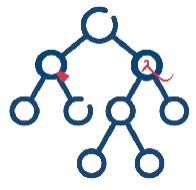
\includegraphics[height=1.0cm]{msca_logo.png}}%
    \end{center}

    \vspace{0.6cm}

    % Main title with Q logos on sides (with clickable links)
    \begin{center}
        \begin{minipage}{0.1\textwidth}
            \centering
            \href{https://quantlet.com}{
\includegraphics[height=1.1cm]{ql_logo.png}}
        \end{minipage}%
        \begin{minipage}{0.78\textwidth}
            \centering
            {\LARGE\bfseries\usebeamercolor[fg]{title}\inserttitle}

            \vspace{0.3cm}

            {\usebeamerfont{subtitle}\usebeamercolor[fg]{title}\insertsubtitle}
        \end{minipage}%
        \begin{minipage}{0.1\textwidth}
            \centering
            \href{https://quantinar.com}{
\includegraphics[height=1.1cm]{qr_logo.png}}
        \end{minipage}
    \end{center}

    \vspace{0.6cm}

    % Authors (left aligned)
    \hspace{0.5cm}{\usebeamerfont{author}\insertauthor}

    \vspace{0.3cm}

    % Institute/Affiliations (left aligned)
    \hspace{0.5cm}\begin{minipage}[t]{0.9\textwidth}
        \raggedright\small\insertinstitute
    \end{minipage}
}

%=============================================================================
% THEOREM ENVIRONMENTS
%=============================================================================
\theoremstyle{definition}
\setbeamertemplate{theorems}[numbered]
\ifdefined\atslang
\newtheorem{defn}{Definiție}
\newtheorem{thm}{Teoremă}
\newtheorem{prop}{Propoziție}
\newtheorem{rmk}{Observație}
\else
\newtheorem{defn}{Definition}
\newtheorem{thm}{Theorem}
\newtheorem{prop}{Proposition}
\newtheorem{rmk}{Remark}
\fi

%=============================================================================
% CENTRED MINIPAGE (no extra vertical space)
%=============================================================================
\newenvironment{cminipage}[1]{%
    \par\noindent\hfill\begin{minipage}{#1}\ignorespaces
}{%
    \end{minipage}\hfill\null\par
}

%=============================================================================
% CUSTOM COMMANDS
%=============================================================================
\newcommand{\E}{\mathbb{E}}
\newcommand{\Var}{\text{Var}}
\newcommand{\Cov}{\text{Cov}}
\newcommand{\Corr}{\text{Corr}}
\newcommand{\R}{\mathbb{R}}
\newcommand{\N}{\mathbb{N}}
\newcommand{\Z}{\mathbb{Z}}
\newcommand{\B}{\mathbf{B}}
\newcommand{\imark}{\textcolor{MainBlue}{\textbullet}}
\newcommand{\RMSE}{\text{RMSE}}
\newcommand{\MAE}{\text{MAE}}
\newcommand{\MAPE}{\text{MAPE}}

% Boldface vector/matrix commands (VAR, VECM, state space)
\newcommand{\bY}{\mathbf{Y}}
\newcommand{\bX}{\mathbf{X}}
\newcommand{\bA}{\mathbf{A}}
\newcommand{\bB}{\mathbf{B}}
\newcommand{\bepsilon}{\boldsymbol{\varepsilon}}
\newcommand{\bSigma}{\boldsymbol{\Sigma}}
\newcommand{\bPhi}{\boldsymbol{\Phi}}
\newcommand{\bGamma}{\boldsymbol{\Gamma}}
\newcommand{\bPi}{\boldsymbol{\Pi}}
\newcommand{\bc}{\mathbf{c}}
\newcommand{\balpha}{\boldsymbol{\alpha}}
\newcommand{\bbeta}{\boldsymbol{\beta}}
\newcommand{\bvarepsilon}{\boldsymbol{\varepsilon}}

% Seminar marks
\newcommand{\correct}{\textcolor{Forest}{\checkmark}}
\newcommand{\incorrect}{\textcolor{Crimson}{\texttimes}}
 se definește
%   \newcommand{\coursename}{Advanced Time Series Analysis and Forecasting}          (EN)
%   \newcommand{\coursename}{Analiza avansată a seriilor de timp și previziune}       (RO)  și  \def\atslang{ro}
% Fișierele .tex se află în EN/Courses, EN/Seminars, RO/Cursuri, RO/Seminarii (două niveluri sub rădăcină).
% Deck-urile sînt generate de latex/build_chapterN.py / build_seminarN.py (vezi latex/ats_build.py).

\documentclass[9pt, aspectratio=169, t]{beamer}
\providecommand{\coursename}{Advanced Time Series Analysis and Forecasting}

% Ensure content fits on slides
\setbeamersize{text margin left=8mm, text margin right=8mm}
% Smaller institute font (title page)
\setbeamerfont{institute}{size=\footnotesize}

%=============================================================================
% THEME AND STYLE CONFIGURATION
%=============================================================================
\usetheme{default}
% Using default theme for clean header/footer control

% Color Palette (matching Redispatch PDF)
\definecolor{MainBlue}{RGB}{26, 58, 110}
\definecolor{AccentBlue}{RGB}{26, 58, 110}
\definecolor{IDAred}{RGB}{205, 0, 0}
\definecolor{DarkGray}{RGB}{51, 51, 51}
\definecolor{MediumGray}{RGB}{128, 128, 128}
\definecolor{LightGray}{RGB}{248, 248, 248}
\definecolor{VeryLightGray}{RGB}{235, 235, 235}
\definecolor{KeynoteGray}{RGB}{218, 218, 218}
\definecolor{SectionGray}{RGB}{120, 120, 120}
\definecolor{FooterGray}{RGB}{100, 100, 100}
\definecolor{Crimson}{RGB}{220, 53, 69}
\definecolor{Forest}{RGB}{46, 125, 50}
\definecolor{Amber}{RGB}{181, 133, 63}
\definecolor{Orange}{RGB}{230, 126, 34}
\definecolor{Purple}{RGB}{142, 68, 173}

% Gradient background (exact Keynote 315° gradient: white to RGB 218,218,218)
\setbeamertemplate{background}{%
    \begin{tikzpicture}[remember picture, overlay]
        \shade[shading=axis, shading angle=315,
        top color=white, bottom color=KeynoteGray]
        (current page.south west) rectangle (current page.north east);
    \end{tikzpicture}%
}
% Fallback solid color for compatibility
\setbeamercolor{background canvas}{bg=}

\setbeamercolor{palette primary}{bg=MainBlue, fg=white}
\setbeamercolor{palette secondary}{bg=MainBlue!85, fg=white}
\setbeamercolor{palette tertiary}{bg=MainBlue!70, fg=white}
\setbeamercolor{structure}{fg=MainBlue}
\setbeamercolor{title}{fg=IDAred}
\setbeamercolor{frametitle}{fg=IDAred, bg=}
\setbeamercolor{block title}{bg=MainBlue, fg=white}
\setbeamercolor{block body}{bg=VeryLightGray, fg=DarkGray}
\setbeamercolor{block title alerted}{bg=Crimson, fg=white}
\setbeamercolor{block body alerted}{bg=Crimson!8, fg=DarkGray}
\setbeamercolor{block title example}{bg=Forest, fg=white}
\setbeamercolor{block body example}{bg=Forest!8, fg=DarkGray}
\setbeamercolor{item}{fg=MainBlue}

% Footer colors (override Madrid theme blue)
\setbeamercolor{author in head/foot}{fg=FooterGray, bg=}
\setbeamercolor{title in head/foot}{fg=FooterGray, bg=}
\setbeamercolor{date in head/foot}{fg=FooterGray, bg=}
\setbeamercolor{section in head/foot}{fg=FooterGray, bg=}
\setbeamercolor{subsection in head/foot}{fg=FooterGray, bg=}

% Bullet styles (apply everywhere including blocks)
\setbeamertemplate{itemize item}{\color{MainBlue}$\boxdot$}
\setbeamertemplate{itemize subitem}{\color{MainBlue}$\blacktriangleright$}
\setbeamertemplate{itemize subsubitem}{\color{MainBlue}\tiny$\bullet$}
\setbeamertemplate{itemize/enumerate body begin}{\normalsize}
\setbeamertemplate{itemize/enumerate subbody begin}{\normalsize}

% Item spacing - compact style
\setlength{\leftmargini}{10pt}       % Level 1: minimal indent
\setlength{\leftmarginii}{10pt}      % Level 2: minimal additional indent
% Compact list spacing (zero extra space before/after lists in blocks)
\makeatletter
\def\@listi{\leftmargin\leftmargini \topsep 0pt \parsep 0pt \itemsep 0pt}
\def\@listii{\leftmargin\leftmarginii \topsep 0pt \parsep 0pt \itemsep 0pt}
\makeatother

\setbeamertemplate{navigation symbols}{}

%=============================================================================
% CUSTOM HEADLINE
%=============================================================================
\setbeamertemplate{headline}{%
    \vskip10pt%
    \hbox to \paperwidth{%
        \hskip0.5cm%
        {\small\color{FooterGray}\renewcommand{\hyperlink}[2]{##2}\insertsectionhead}%
        \hfill%
        \textcolor{FooterGray}{\small\insertframenumber}%
        \hskip0.5cm%
    }%
    \vskip4pt%
    {\color{FooterGray}\hrule height 0.4pt}%
}

%=============================================================================
% CUSTOM FOOTER
%=============================================================================
\usepackage{fontawesome5}

\setbeamertemplate{footline}{%
    {\color{FooterGray}\hrule height 0.4pt}%
    \vskip4pt%
    \hbox to \paperwidth{%
        \hskip0.5cm%
        \textcolor{FooterGray}{\small\coursename}%
        \hfill%
        \raisebox{-0.1em}{%
            \begin{tikzpicture}[x=0.08em, y=0.08em, line width=0.4pt]
                \draw[FooterGray] (0,3) -- (1,4) -- (2,3.5) -- (3,5) -- (4,4) -- (5,6) -- (6,5.5) -- (7,4) -- (8,5) -- (9,7) -- (10,6) -- (11,5) -- (12,6.5) -- (13,8) -- (14,7) -- (15,6) -- (16,7.5) -- (17,9) -- (18,8) -- (19,7) -- (20,8.5) -- (21,10) -- (22,9) -- (23,8) -- (24,9.5);
            \end{tikzpicture}%
        }%
        \hskip0.5cm%
    }%
    \vskip6pt%
}

%=============================================================================
% PACKAGES
%=============================================================================
\usepackage[utf8]{inputenc}
\DeclareUnicodeCharacter{03B1}{\ensuremath{\alpha}}
\usepackage[T1]{fontenc}
\usepackage{amsmath, amssymb, amsthm}
\usepackage{mathtools}
\usepackage{bm}
\usepackage{tikz}
\usetikzlibrary{arrows.meta, positioning, shapes, calc, decorations.pathreplacing, shadings}
\usepackage{booktabs}
\usepackage{multirow}
\usepackage{array}
\usepackage{graphicx}
\usepackage{animate}
\usepackage{hyperref}
\usepackage{colortbl}
\usepackage{listings}
\lstset{language=Python, basicstyle=\ttfamily\scriptsize, keywordstyle=\color{MainBlue}\bfseries,
  commentstyle=\color{Forest}, stringstyle=\color{Crimson}, breaklines=true,
  frame=none, backgroundcolor=\color{VeryLightGray}, xleftmargin=2mm}
\hypersetup{colorlinks=true, linkcolor=MainBlue, urlcolor=MainBlue}
\graphicspath{{../../logos/}{../../charts/}{../../photos/}}
\usepackage{xcolor}
\hfuzz=2pt  % Suppress tiny overfull warnings (<2pt)
\vfuzz=2pt  % Suppress tiny vertical overfull warnings (<2pt)

%=============================================================================
% QUANTLET COMMANDS
%   \quantlet{<displayed name>}{<url>}       (generic)
%   \atsquantlet{Ch_05}{ATS_ch5_garch}       -> https://github.com/danpele/Advanced-Time-Series/tree/main/Quantlets/Ch_05/ATS_ch5_garch
%   \qlurl{<folder>} is defined per chapter by the generator (Quantlets/Ch_NN/<folder>)
%=============================================================================
\newcommand{\atsrepo}{https://github.com/danpele/Advanced-Time-Series}
\newcommand{\atsqlbase}{https://github.com/danpele/Advanced-Time-Series/tree/main/Quantlets}
\newcommand{\quantlet}[2]{%
    \hfill\href{#2}{%
        \raisebox{-0.15em}{
\includegraphics[height=0.7em]{ql_logo.png}}%
        \textcolor{MainBlue}{\tiny\ #1}%
    }%
}
\newcommand{\atsquantlet}[2]{\quantlet{\detokenize{#2}}{\atsqlbase/#1/#2}}

%=============================================================================
% NOTEBOOKS (Google Colab)
%   \colaburl{notebooks/EN/chapter5_seminar_notebook.ipynb} -> the Colab link of a file in the ATS repo
%   \nb: the chapter notebook (each seminar deck redefines it with \renewcommand)
%=============================================================================
\newcommand{\colaburl}[1]{https://colab.research.google.com/github/danpele/Advanced-Time-Series/blob/main/#1}
\newcommand{\nb}{https://colab.research.google.com/github/danpele/Advanced-Time-Series/tree/main/notebooks/EN}
\newcommand{\nbname}{notebooks/EN}

%=============================================================================
% SLIDE HELPERS (used by the generators; the same as in MFM)
%=============================================================================
% local font size for list bodies (the preamble forces \normalsize)
\newcommand{\itemsize}[1]{\setbeamertemplate{itemize/enumerate body begin}{#1}\setbeamertemplate{itemize/enumerate subbody begin}{#1}}
\newcommand{\intitle}[1]{{\hypersetup{urlcolor=white}#1}}   % white links inside coloured title bars
\newcommand{\imgcap}[1]{{\scriptsize #1}\\[0.5mm]}          % caption under a photo
\newcommand{\imgcredit}[2]{{\tiny\color{FooterGray}\href{#1}{#2}}}   % image credit: source URL, author/licence
\newcommand{\aiprompt}[1]{{\ttfamily\color{MainBlue}#1}}     % a prompt to an AI assistant

%=============================================================================
% SEMINARS: student version by default; the instructor wrapper *_solutions.tex sets \solutionstrue
%=============================================================================
\makeatletter\@ifundefined{ifsolutions}{\expandafter\newif\csname ifsolutions\endcsname}{}\makeatother
\newcommand{\solonly}[1]{\ifsolutions #1\fi}
\newcommand{\propsub}{\ifsolutions\else\framesubtitle{\ifdefined\atslang Rezolvarea se discută la seminar\else Solution discussed in class\fi}\fi}

%=============================================================================
% APPENDIX AND CHAPTER LINKS (latex/appendix_links.py writes the calls; it also re-declares these
% macros before \begin{document}, so the decks compile with or without this preamble block)
%=============================================================================
\providecommand{\atsapplink}[3]{\hypertarget{#2}{}\hyperlink{#1}{\beamergotobutton{#3}}}
\providecommand{\atsappback}[2]{\begin{tikzpicture}[remember picture,overlay]\node[anchor=south east] at ([xshift=-3mm,yshift=7mm]current page.south east){\hyperlink{#1}{\beamerreturnbutton{#2}}};\end{tikzpicture}}
\providecommand{\atschlink}[2]{\href{#1}{#2}}
\providecommand{\atschlinkt}[2]{\href{#1}{\usebeamercolor[fg]{frametitle}#2}}

%=============================================================================
% QUANTINAR COMMAND: link către un curs Quantinar (subiecte avansate)
%=============================================================================
\newcommand{\quantinar}[2]{%
    \href{#2}{%
        \raisebox{-0.15em}{
\includegraphics[height=0.8em]{qr_logo.png}}%
        \textcolor{MainBlue}{\scriptsize\ #1}%
    }%
}

%=============================================================================
% CUSTOM TITLE PAGE
%=============================================================================
\defbeamertemplate*{title page}{hybrid}[1][]
{
    \vspace{0.2cm}
    % Logos row - top header (with clickable links)
    \begin{center}
        \href{https://www.ase.ro}{
\includegraphics[height=1.0cm]{ase_logo.png}}\hspace{0.3cm}%
        \href{https://theida.net}{
\includegraphics[height=1.0cm]{ida_logo.png}}\hspace{0.3cm}%
        \href{https://blockchain-research-center.com}{
\includegraphics[height=1.0cm]{brc_logo.png}}\hspace{0.3cm}%
        \href{https://www.ai4efin.ase.ro}{
\includegraphics[height=1.0cm]{ai4efin_logo.png}}\hspace{0.3cm}%
        \href{https://ipe.ro/new}{
\includegraphics[height=1.0cm]{acad_logo.png}}\hspace{0.3cm}%
        \href{https://www.digital-finance-msca.com}{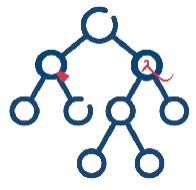
\includegraphics[height=1.0cm]{msca_logo.png}}%
    \end{center}

    \vspace{0.6cm}

    % Main title with Q logos on sides (with clickable links)
    \begin{center}
        \begin{minipage}{0.1\textwidth}
            \centering
            \href{https://quantlet.com}{
\includegraphics[height=1.1cm]{ql_logo.png}}
        \end{minipage}%
        \begin{minipage}{0.78\textwidth}
            \centering
            {\LARGE\bfseries\usebeamercolor[fg]{title}\inserttitle}

            \vspace{0.3cm}

            {\usebeamerfont{subtitle}\usebeamercolor[fg]{title}\insertsubtitle}
        \end{minipage}%
        \begin{minipage}{0.1\textwidth}
            \centering
            \href{https://quantinar.com}{
\includegraphics[height=1.1cm]{qr_logo.png}}
        \end{minipage}
    \end{center}

    \vspace{0.6cm}

    % Authors (left aligned)
    \hspace{0.5cm}{\usebeamerfont{author}\insertauthor}

    \vspace{0.3cm}

    % Institute/Affiliations (left aligned)
    \hspace{0.5cm}\begin{minipage}[t]{0.9\textwidth}
        \raggedright\small\insertinstitute
    \end{minipage}
}

%=============================================================================
% THEOREM ENVIRONMENTS
%=============================================================================
\theoremstyle{definition}
\setbeamertemplate{theorems}[numbered]
\ifdefined\atslang
\newtheorem{defn}{Definiție}
\newtheorem{thm}{Teoremă}
\newtheorem{prop}{Propoziție}
\newtheorem{rmk}{Observație}
\else
\newtheorem{defn}{Definition}
\newtheorem{thm}{Theorem}
\newtheorem{prop}{Proposition}
\newtheorem{rmk}{Remark}
\fi

%=============================================================================
% CENTRED MINIPAGE (no extra vertical space)
%=============================================================================
\newenvironment{cminipage}[1]{%
    \par\noindent\hfill\begin{minipage}{#1}\ignorespaces
}{%
    \end{minipage}\hfill\null\par
}

%=============================================================================
% CUSTOM COMMANDS
%=============================================================================
\newcommand{\E}{\mathbb{E}}
\newcommand{\Var}{\text{Var}}
\newcommand{\Cov}{\text{Cov}}
\newcommand{\Corr}{\text{Corr}}
\newcommand{\R}{\mathbb{R}}
\newcommand{\N}{\mathbb{N}}
\newcommand{\Z}{\mathbb{Z}}
\newcommand{\B}{\mathbf{B}}
\newcommand{\imark}{\textcolor{MainBlue}{\textbullet}}
\newcommand{\RMSE}{\text{RMSE}}
\newcommand{\MAE}{\text{MAE}}
\newcommand{\MAPE}{\text{MAPE}}

% Boldface vector/matrix commands (VAR, VECM, state space)
\newcommand{\bY}{\mathbf{Y}}
\newcommand{\bX}{\mathbf{X}}
\newcommand{\bA}{\mathbf{A}}
\newcommand{\bB}{\mathbf{B}}
\newcommand{\bepsilon}{\boldsymbol{\varepsilon}}
\newcommand{\bSigma}{\boldsymbol{\Sigma}}
\newcommand{\bPhi}{\boldsymbol{\Phi}}
\newcommand{\bGamma}{\boldsymbol{\Gamma}}
\newcommand{\bPi}{\boldsymbol{\Pi}}
\newcommand{\bc}{\mathbf{c}}
\newcommand{\balpha}{\boldsymbol{\alpha}}
\newcommand{\bbeta}{\boldsymbol{\beta}}
\newcommand{\bvarepsilon}{\boldsymbol{\varepsilon}}

% Seminar marks
\newcommand{\correct}{\textcolor{Forest}{\checkmark}}
\newcommand{\incorrect}{\textcolor{Crimson}{\texttimes}}
 se definește
%   \newcommand{\coursename}{Advanced Time Series Analysis and Forecasting}          (EN)
%   \newcommand{\coursename}{Analiza avansată a seriilor de timp și previziune}       (RO)  și  \def\atslang{ro}
% Fișierele .tex se află în EN/Courses, EN/Seminars, RO/Cursuri, RO/Seminarii (două niveluri sub rădăcină).
% Deck-urile sînt generate de latex/build_chapterN.py / build_seminarN.py (vezi latex/ats_build.py).

\documentclass[9pt, aspectratio=169, t]{beamer}
\providecommand{\coursename}{Advanced Time Series Analysis and Forecasting}

% Ensure content fits on slides
\setbeamersize{text margin left=8mm, text margin right=8mm}
% Smaller institute font (title page)
\setbeamerfont{institute}{size=\footnotesize}

%=============================================================================
% THEME AND STYLE CONFIGURATION
%=============================================================================
\usetheme{default}
% Using default theme for clean header/footer control

% Color Palette (matching Redispatch PDF)
\definecolor{MainBlue}{RGB}{26, 58, 110}
\definecolor{AccentBlue}{RGB}{26, 58, 110}
\definecolor{IDAred}{RGB}{205, 0, 0}
\definecolor{DarkGray}{RGB}{51, 51, 51}
\definecolor{MediumGray}{RGB}{128, 128, 128}
\definecolor{LightGray}{RGB}{248, 248, 248}
\definecolor{VeryLightGray}{RGB}{235, 235, 235}
\definecolor{KeynoteGray}{RGB}{218, 218, 218}
\definecolor{SectionGray}{RGB}{120, 120, 120}
\definecolor{FooterGray}{RGB}{100, 100, 100}
\definecolor{Crimson}{RGB}{220, 53, 69}
\definecolor{Forest}{RGB}{46, 125, 50}
\definecolor{Amber}{RGB}{181, 133, 63}
\definecolor{Orange}{RGB}{230, 126, 34}
\definecolor{Purple}{RGB}{142, 68, 173}

% Gradient background (exact Keynote 315° gradient: white to RGB 218,218,218)
\setbeamertemplate{background}{%
    \begin{tikzpicture}[remember picture, overlay]
        \shade[shading=axis, shading angle=315,
        top color=white, bottom color=KeynoteGray]
        (current page.south west) rectangle (current page.north east);
    \end{tikzpicture}%
}
% Fallback solid color for compatibility
\setbeamercolor{background canvas}{bg=}

\setbeamercolor{palette primary}{bg=MainBlue, fg=white}
\setbeamercolor{palette secondary}{bg=MainBlue!85, fg=white}
\setbeamercolor{palette tertiary}{bg=MainBlue!70, fg=white}
\setbeamercolor{structure}{fg=MainBlue}
\setbeamercolor{title}{fg=IDAred}
\setbeamercolor{frametitle}{fg=IDAred, bg=}
\setbeamercolor{block title}{bg=MainBlue, fg=white}
\setbeamercolor{block body}{bg=VeryLightGray, fg=DarkGray}
\setbeamercolor{block title alerted}{bg=Crimson, fg=white}
\setbeamercolor{block body alerted}{bg=Crimson!8, fg=DarkGray}
\setbeamercolor{block title example}{bg=Forest, fg=white}
\setbeamercolor{block body example}{bg=Forest!8, fg=DarkGray}
\setbeamercolor{item}{fg=MainBlue}

% Footer colors (override Madrid theme blue)
\setbeamercolor{author in head/foot}{fg=FooterGray, bg=}
\setbeamercolor{title in head/foot}{fg=FooterGray, bg=}
\setbeamercolor{date in head/foot}{fg=FooterGray, bg=}
\setbeamercolor{section in head/foot}{fg=FooterGray, bg=}
\setbeamercolor{subsection in head/foot}{fg=FooterGray, bg=}

% Bullet styles (apply everywhere including blocks)
\setbeamertemplate{itemize item}{\color{MainBlue}$\boxdot$}
\setbeamertemplate{itemize subitem}{\color{MainBlue}$\blacktriangleright$}
\setbeamertemplate{itemize subsubitem}{\color{MainBlue}\tiny$\bullet$}
\setbeamertemplate{itemize/enumerate body begin}{\normalsize}
\setbeamertemplate{itemize/enumerate subbody begin}{\normalsize}

% Item spacing - compact style
\setlength{\leftmargini}{10pt}       % Level 1: minimal indent
\setlength{\leftmarginii}{10pt}      % Level 2: minimal additional indent
% Compact list spacing (zero extra space before/after lists in blocks)
\makeatletter
\def\@listi{\leftmargin\leftmargini \topsep 0pt \parsep 0pt \itemsep 0pt}
\def\@listii{\leftmargin\leftmarginii \topsep 0pt \parsep 0pt \itemsep 0pt}
\makeatother

\setbeamertemplate{navigation symbols}{}

%=============================================================================
% CUSTOM HEADLINE
%=============================================================================
\setbeamertemplate{headline}{%
    \vskip10pt%
    \hbox to \paperwidth{%
        \hskip0.5cm%
        {\small\color{FooterGray}\renewcommand{\hyperlink}[2]{##2}\insertsectionhead}%
        \hfill%
        \textcolor{FooterGray}{\small\insertframenumber}%
        \hskip0.5cm%
    }%
    \vskip4pt%
    {\color{FooterGray}\hrule height 0.4pt}%
}

%=============================================================================
% CUSTOM FOOTER
%=============================================================================
\usepackage{fontawesome5}

\setbeamertemplate{footline}{%
    {\color{FooterGray}\hrule height 0.4pt}%
    \vskip4pt%
    \hbox to \paperwidth{%
        \hskip0.5cm%
        \textcolor{FooterGray}{\small\coursename}%
        \hfill%
        \raisebox{-0.1em}{%
            \begin{tikzpicture}[x=0.08em, y=0.08em, line width=0.4pt]
                \draw[FooterGray] (0,3) -- (1,4) -- (2,3.5) -- (3,5) -- (4,4) -- (5,6) -- (6,5.5) -- (7,4) -- (8,5) -- (9,7) -- (10,6) -- (11,5) -- (12,6.5) -- (13,8) -- (14,7) -- (15,6) -- (16,7.5) -- (17,9) -- (18,8) -- (19,7) -- (20,8.5) -- (21,10) -- (22,9) -- (23,8) -- (24,9.5);
            \end{tikzpicture}%
        }%
        \hskip0.5cm%
    }%
    \vskip6pt%
}

%=============================================================================
% PACKAGES
%=============================================================================
\usepackage[utf8]{inputenc}
\DeclareUnicodeCharacter{03B1}{\ensuremath{\alpha}}
\usepackage[T1]{fontenc}
\usepackage{amsmath, amssymb, amsthm}
\usepackage{mathtools}
\usepackage{bm}
\usepackage{tikz}
\usetikzlibrary{arrows.meta, positioning, shapes, calc, decorations.pathreplacing, shadings}
\usepackage{booktabs}
\usepackage{multirow}
\usepackage{array}
\usepackage{graphicx}
\usepackage{animate}
\usepackage{hyperref}
\usepackage{colortbl}
\usepackage{listings}
\lstset{language=Python, basicstyle=\ttfamily\scriptsize, keywordstyle=\color{MainBlue}\bfseries,
  commentstyle=\color{Forest}, stringstyle=\color{Crimson}, breaklines=true,
  frame=none, backgroundcolor=\color{VeryLightGray}, xleftmargin=2mm}
\hypersetup{colorlinks=true, linkcolor=MainBlue, urlcolor=MainBlue}
\graphicspath{{../../logos/}{../../charts/}{../../photos/}}
\usepackage{xcolor}
\hfuzz=2pt  % Suppress tiny overfull warnings (<2pt)
\vfuzz=2pt  % Suppress tiny vertical overfull warnings (<2pt)

%=============================================================================
% QUANTLET COMMANDS
%   \quantlet{<displayed name>}{<url>}       (generic)
%   \atsquantlet{Ch_05}{ATS_ch5_garch}       -> https://github.com/danpele/Advanced-Time-Series/tree/main/Quantlets/Ch_05/ATS_ch5_garch
%   \qlurl{<folder>} is defined per chapter by the generator (Quantlets/Ch_NN/<folder>)
%=============================================================================
\newcommand{\atsrepo}{https://github.com/danpele/Advanced-Time-Series}
\newcommand{\atsqlbase}{https://github.com/danpele/Advanced-Time-Series/tree/main/Quantlets}
\newcommand{\quantlet}[2]{%
    \hfill\href{#2}{%
        \raisebox{-0.15em}{
\includegraphics[height=0.7em]{ql_logo.png}}%
        \textcolor{MainBlue}{\tiny\ #1}%
    }%
}
\newcommand{\atsquantlet}[2]{\quantlet{\detokenize{#2}}{\atsqlbase/#1/#2}}

%=============================================================================
% NOTEBOOKS (Google Colab)
%   \colaburl{notebooks/EN/chapter5_seminar_notebook.ipynb} -> the Colab link of a file in the ATS repo
%   \nb: the chapter notebook (each seminar deck redefines it with \renewcommand)
%=============================================================================
\newcommand{\colaburl}[1]{https://colab.research.google.com/github/danpele/Advanced-Time-Series/blob/main/#1}
\newcommand{\nb}{https://colab.research.google.com/github/danpele/Advanced-Time-Series/tree/main/notebooks/EN}
\newcommand{\nbname}{notebooks/EN}

%=============================================================================
% SLIDE HELPERS (used by the generators; the same as in MFM)
%=============================================================================
% local font size for list bodies (the preamble forces \normalsize)
\newcommand{\itemsize}[1]{\setbeamertemplate{itemize/enumerate body begin}{#1}\setbeamertemplate{itemize/enumerate subbody begin}{#1}}
\newcommand{\intitle}[1]{{\hypersetup{urlcolor=white}#1}}   % white links inside coloured title bars
\newcommand{\imgcap}[1]{{\scriptsize #1}\\[0.5mm]}          % caption under a photo
\newcommand{\imgcredit}[2]{{\tiny\color{FooterGray}\href{#1}{#2}}}   % image credit: source URL, author/licence
\newcommand{\aiprompt}[1]{{\ttfamily\color{MainBlue}#1}}     % a prompt to an AI assistant

%=============================================================================
% SEMINARS: student version by default; the instructor wrapper *_solutions.tex sets \solutionstrue
%=============================================================================
\makeatletter\@ifundefined{ifsolutions}{\expandafter\newif\csname ifsolutions\endcsname}{}\makeatother
\newcommand{\solonly}[1]{\ifsolutions #1\fi}
\newcommand{\propsub}{\ifsolutions\else\framesubtitle{\ifdefined\atslang Rezolvarea se discută la seminar\else Solution discussed in class\fi}\fi}

%=============================================================================
% APPENDIX AND CHAPTER LINKS (latex/appendix_links.py writes the calls; it also re-declares these
% macros before \begin{document}, so the decks compile with or without this preamble block)
%=============================================================================
\providecommand{\atsapplink}[3]{\hypertarget{#2}{}\hyperlink{#1}{\beamergotobutton{#3}}}
\providecommand{\atsappback}[2]{\begin{tikzpicture}[remember picture,overlay]\node[anchor=south east] at ([xshift=-3mm,yshift=7mm]current page.south east){\hyperlink{#1}{\beamerreturnbutton{#2}}};\end{tikzpicture}}
\providecommand{\atschlink}[2]{\href{#1}{#2}}
\providecommand{\atschlinkt}[2]{\href{#1}{\usebeamercolor[fg]{frametitle}#2}}

%=============================================================================
% QUANTINAR COMMAND: link către un curs Quantinar (subiecte avansate)
%=============================================================================
\newcommand{\quantinar}[2]{%
    \href{#2}{%
        \raisebox{-0.15em}{
\includegraphics[height=0.8em]{qr_logo.png}}%
        \textcolor{MainBlue}{\scriptsize\ #1}%
    }%
}

%=============================================================================
% CUSTOM TITLE PAGE
%=============================================================================
\defbeamertemplate*{title page}{hybrid}[1][]
{
    \vspace{0.2cm}
    % Logos row - top header (with clickable links)
    \begin{center}
        \href{https://www.ase.ro}{
\includegraphics[height=1.0cm]{ase_logo.png}}\hspace{0.3cm}%
        \href{https://theida.net}{
\includegraphics[height=1.0cm]{ida_logo.png}}\hspace{0.3cm}%
        \href{https://blockchain-research-center.com}{
\includegraphics[height=1.0cm]{brc_logo.png}}\hspace{0.3cm}%
        \href{https://www.ai4efin.ase.ro}{
\includegraphics[height=1.0cm]{ai4efin_logo.png}}\hspace{0.3cm}%
        \href{https://ipe.ro/new}{
\includegraphics[height=1.0cm]{acad_logo.png}}\hspace{0.3cm}%
        \href{https://www.digital-finance-msca.com}{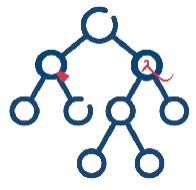
\includegraphics[height=1.0cm]{msca_logo.png}}%
    \end{center}

    \vspace{0.6cm}

    % Main title with Q logos on sides (with clickable links)
    \begin{center}
        \begin{minipage}{0.1\textwidth}
            \centering
            \href{https://quantlet.com}{
\includegraphics[height=1.1cm]{ql_logo.png}}
        \end{minipage}%
        \begin{minipage}{0.78\textwidth}
            \centering
            {\LARGE\bfseries\usebeamercolor[fg]{title}\inserttitle}

            \vspace{0.3cm}

            {\usebeamerfont{subtitle}\usebeamercolor[fg]{title}\insertsubtitle}
        \end{minipage}%
        \begin{minipage}{0.1\textwidth}
            \centering
            \href{https://quantinar.com}{
\includegraphics[height=1.1cm]{qr_logo.png}}
        \end{minipage}
    \end{center}

    \vspace{0.6cm}

    % Authors (left aligned)
    \hspace{0.5cm}{\usebeamerfont{author}\insertauthor}

    \vspace{0.3cm}

    % Institute/Affiliations (left aligned)
    \hspace{0.5cm}\begin{minipage}[t]{0.9\textwidth}
        \raggedright\small\insertinstitute
    \end{minipage}
}

%=============================================================================
% THEOREM ENVIRONMENTS
%=============================================================================
\theoremstyle{definition}
\setbeamertemplate{theorems}[numbered]
\ifdefined\atslang
\newtheorem{defn}{Definiție}
\newtheorem{thm}{Teoremă}
\newtheorem{prop}{Propoziție}
\newtheorem{rmk}{Observație}
\else
\newtheorem{defn}{Definition}
\newtheorem{thm}{Theorem}
\newtheorem{prop}{Proposition}
\newtheorem{rmk}{Remark}
\fi

%=============================================================================
% CENTRED MINIPAGE (no extra vertical space)
%=============================================================================
\newenvironment{cminipage}[1]{%
    \par\noindent\hfill\begin{minipage}{#1}\ignorespaces
}{%
    \end{minipage}\hfill\null\par
}

%=============================================================================
% CUSTOM COMMANDS
%=============================================================================
\newcommand{\E}{\mathbb{E}}
\newcommand{\Var}{\text{Var}}
\newcommand{\Cov}{\text{Cov}}
\newcommand{\Corr}{\text{Corr}}
\newcommand{\R}{\mathbb{R}}
\newcommand{\N}{\mathbb{N}}
\newcommand{\Z}{\mathbb{Z}}
\newcommand{\B}{\mathbf{B}}
\newcommand{\imark}{\textcolor{MainBlue}{\textbullet}}
\newcommand{\RMSE}{\text{RMSE}}
\newcommand{\MAE}{\text{MAE}}
\newcommand{\MAPE}{\text{MAPE}}

% Boldface vector/matrix commands (VAR, VECM, state space)
\newcommand{\bY}{\mathbf{Y}}
\newcommand{\bX}{\mathbf{X}}
\newcommand{\bA}{\mathbf{A}}
\newcommand{\bB}{\mathbf{B}}
\newcommand{\bepsilon}{\boldsymbol{\varepsilon}}
\newcommand{\bSigma}{\boldsymbol{\Sigma}}
\newcommand{\bPhi}{\boldsymbol{\Phi}}
\newcommand{\bGamma}{\boldsymbol{\Gamma}}
\newcommand{\bPi}{\boldsymbol{\Pi}}
\newcommand{\bc}{\mathbf{c}}
\newcommand{\balpha}{\boldsymbol{\alpha}}
\newcommand{\bbeta}{\boldsymbol{\beta}}
\newcommand{\bvarepsilon}{\boldsymbol{\varepsilon}}

% Seminar marks
\newcommand{\correct}{\textcolor{Forest}{\checkmark}}
\newcommand{\incorrect}{\textcolor{Crimson}{\texttimes}}


\newcommand{\qlurl}[1]{https://github.com/danpele/Advanced-Time-Series/tree/main/Quantlets/Ch_10/#1}

% Clickable citations (DOIs verified via Crossref)
\newcommand{\refABDL}{\href{https://doi.org/10.1111/1468-0262.00418}{Andersen et al.\ (2003)}}
\newcommand{\refAnSu}{\href{https://doi.org/10.1111/j.1468-0262.2004.00501.x}{Andrews and Sun (2004)}}
\newcommand{\refBBM}{\href{https://doi.org/10.1016/S0304-4076(95)01749-6}{Baillie, Bollerslev and Mikkelsen (1996)}}
\newcommand{\refBCT}{\href{https://doi.org/10.1002/(SICI)1099-1255(199601)11:1\%3C23::AID-JAE374\%3E3.0.CO;2-M}{Baillie, Chung and Tieslau (1996)}}
\newcommand{\refBP}{\href{https://doi.org/10.1093/jjfinec/nbl003}{Bandi and Perron (2006)}}
\newcommand{\refBFG}{\href{https://doi.org/10.1080/14697688.2015.1099717}{Bayer, Friz and Gatheral (2016)}}
\newcommand{\refBLPa}{\href{https://doi.org/10.1007/s00780-017-0335-5}{Bennedsen, Lunde and Pakkanen (2017)}}
\newcommand{\refBLPb}{\href{https://doi.org/10.1093/jjfinec/nbaa049}{Bennedsen, Lunde and Pakkanen (2022)}}
\newcommand{\refBFGK}{\href{https://doi.org/10.1007/978-3-642-35512-7}{Beran et al.\ (2013)}}
\newcommand{\refBCPV}{\href{https://doi.org/10.1016/j.jeconom.2022.06.009}{Bolko et al.\ (2023)}}
\newcommand{\refBCL}{\href{https://doi.org/10.1016/S0304-4076(97)00072-9}{Breidt, Crato and de Lima (1998)}}
\newcommand{\refCN}{\href{https://doi.org/10.1016/j.jeconom.2005.03.018}{Christensen and Nielsen (2006)}}
\newcommand{\refCR}{\href{https://doi.org/10.1111/1467-9965.00057}{Comte and Renault (1998)}}
\newcommand{\refCD}{\href{https://doi.org/10.1007/s13571-024-00322-2}{Cont and Das (2024)}}
\newcommand{\refCor}{\href{https://doi.org/10.1093/jjfinec/nbp001}{Corsi (2009)}}
\newcommand{\refDav}{\href{https://doi.org/10.1198/073500103288619359}{Davidson (2004)}}
\newcommand{\refDH}{\href{https://doi.org/10.1093/biomet/74.1.95}{Davies and Harte (1987)}}
\newcommand{\refDI}{\href{https://doi.org/10.1016/S0304-4076(01)00073-2}{Diebold and Inoue (2001)}}
\newcommand{\refDM}{\href{https://doi.org/10.1080/07350015.1995.10524599}{Diebold and Mariano (1995)}}
\newcommand{\refDN}{\href{https://doi.org/10.1137/S1064827592240555}{Dietrich and Newsam (1997)}}
\newcommand{\refER}{\href{https://doi.org/10.1111/mafi.12173}{El Euch and Rosenbaum (2019)}}
\newcommand{\refFT}{\href{https://doi.org/10.1214/aos/1176349936}{Fox and Taqqu (1986)}}
\newcommand{\refFTW}{\href{https://doi.org/10.1111/mafi.12354}{Fukasawa, Takabatake and Westphal (2022)}}
\newcommand{\refGJR}{\href{https://doi.org/10.1080/14697688.2017.1393551}{Gatheral, Jaisson and Rosenbaum (2018)}}
\newcommand{\refGPH}{\href{https://doi.org/10.1111/j.1467-9892.1983.tb00371.x}{Geweke and Porter-Hudak (1983)}}
\newcommand{\refGS}{\href{https://doi.org/10.1137/S0036144501394387}{Gneiting and Schlather (2004)}}
\newcommand{\refGra}{\href{https://doi.org/10.1016/0304-4076(80)90092-5}{Granger (1980)}}
\newcommand{\refGH}{\href{https://doi.org/10.1016/j.jempfin.2003.03.001}{Granger and Hyung (2004)}}
\newcommand{\refGJ}{\href{https://doi.org/10.1111/j.1467-9892.1980.tb00297.x}{Granger and Joyeux (1980)}}
\newcommand{\refHW}{\href{https://doi.org/10.1080/07350015.1995.10524577}{Hassler and Wolters (1995)}}
\newcommand{\refOMI}{\href{https://web.archive.org/web/20220301022212/https://realized.oxford-man.ox.ac.uk/}{Heber et al.\ (2009)}}
\newcommand{\refHR}{\href{https://doi.org/10.1007/978-1-4612-2412-9_16}{Henry and Robinson (1996)}}
\newcommand{\refHos}{\href{https://doi.org/10.1093/biomet/68.1.165}{Hosking (1981)}}
\newcommand{\refHur}{\href{https://doi.org/10.1061/TACEAT.0006518}{Hurst (1951)}}
\newcommand{\refHDB}{\href{https://doi.org/10.1111/1467-9892.00075}{Hurvich, Deo and Brodsky (1998)}}
\newcommand{\refHMS}{\href{https://doi.org/10.1111/j.1468-0262.2005.00616.x}{Hurvich, Moulines and Soulier (2005)}}
\newcommand{\refJN}{\href{https://doi.org/10.3982/ECTA9299}{Johansen and Nielsen (2012)}}
\newcommand{\refLMPR}{\href{https://doi.org/10.1080/24725854.2018.1444297}{Livieri et al.\ (2018)}}
\newcommand{\refLP}{\href{https://doi.org/10.1016/j.jempfin.2009.10.001}{Lu and Perron (2010)}}
\newcommand{\refMN}{\href{https://doi.org/10.1002/jae.2295}{MacKinnon and Nielsen (2014)}}
\newcommand{\refMVN}{\href{https://doi.org/10.1137/1010093}{Mandelbrot and Van Ness (1968)}}
\newcommand{\refNS}{\href{https://doi.org/10.1016/j.jeconom.2006.10.008}{Nielsen and Shimotsu (2007)}}
\newcommand{\refPar}{\href{https://doi.org/10.1086/296071}{Parkinson (1980)}}
\newcommand{\refPat}{\href{https://doi.org/10.1016/j.jeconom.2010.03.034}{Patton (2011)}}
\newcommand{\refPQ}{\href{https://doi.org/10.1198/jbes.2009.06171}{Perron and Qu (2010)}}
\newcommand{\refPet}{\href{https://doi.org/10.1016/j.ijforecast.2021.11.001}{Petropoulos et al.\ (2022)}}
\newcommand{\refPS}{\href{https://doi.org/10.1214/009053604000000139}{Phillips and Shimotsu (2004)}}
\newcommand{\refQu}{\href{https://doi.org/10.1198/jbes.2010.09153}{Qu (2011)}}
\newcommand{\refRobA}{\href{https://doi.org/10.1214/aos/1176325382}{Robinson (1994)}}
\newcommand{\refRobB}{\href{https://doi.org/10.1214/aos/1176324636}{Robinson (1995a)}}
\newcommand{\refRobC}{\href{https://doi.org/10.1214/aos/1176324317}{Robinson (1995b)}}
\newcommand{\refSP}{\href{https://doi.org/10.1214/009053605000000309}{Shimotsu and Phillips (2005)}}
\newcommand{\refShi}{\href{https://doi.org/10.1017/S0266466609100075}{Shimotsu (2010)}}
\newcommand{\refVel}{\href{https://doi.org/10.1111/1467-9892.00127}{Velasco (1999)}}
\newcommand{\refWXY}{\href{https://doi.org/10.1016/j.jeconom.2021.08.001}{Wang, Xiao and Yu (2023)}}

\title[Advanced Time Series Analysis and Forecasting]{Advanced Time Series Analysis and Forecasting}
\subtitle{Chapter 10: Long memory and rough volatility}
\author[D.T. Pele]{Daniel Traian PELE}
\institute{Bucharest University of Economic Studies\\
IDA Institute Digital Assets\\
Blockchain Research Center\\
AI4EFin Artificial Intelligence for Energy Finance\\
Romanian Academy, Institute for Economic Forecasting\\
MSCA Digital Finance}
\date{}

%=============================================================================
\providecommand{\atsapplink}[3]{\hypertarget{#2}{}\hyperlink{#1}{\beamergotobutton{#3}}}  % APPLINKS-MACROS
\providecommand{\atsappback}[2]{\begin{tikzpicture}[remember picture,overlay]\node[anchor=south east] at ([xshift=-3mm,yshift=7mm]current page.south east){\hyperlink{#1}{\beamerreturnbutton{#2}}};\end{tikzpicture}}  % APPLINKS-MACROS
\providecommand{\atschlink}[2]{\href{#1}{#2}}  % APPLINKS-MACROS
\providecommand{\atschlinkt}[2]{\href{#1}{\usebeamercolor[fg]{frametitle}#2}}  % APPLINKS-MACROS
\begin{document}
%=============================================================================

{
\setbeamertemplate{headline}{}
\setbeamertemplate{footline}{}
\begin{frame}[noframenumbering]
    \titlepage
\end{frame}
}
% BEGIN-ACRONYMS (generat de latex/acronyms.py; nu editati manual)
\begin{frame}{Acronyms used in this material (1/2)}
\setbeamertemplate{itemize/enumerate body begin}{\footnotesize}
\begin{columns}[T]
\begin{column}{0.49\textwidth}
\begin{itemize}\setlength{\itemsep}{0pt}
    \item \textbf{ACF}: Autocorrelation Function
    \item \textbf{AI}: Artificial Intelligence
    \item \textbf{AR}: AutoRegressive (model); in event studies: Abnormal Return
    \item \textbf{ARCH}: AutoRegressive Conditional Heteroskedasticity
    \item \textbf{ARFIMA}: AutoRegressive Fractionally Integrated Moving Average (model)
    \item \textbf{ARMA}: AutoRegressive Moving Average (model)
    \item \textbf{BET}: Bucharest Exchange Trading (index)
    \item \textbf{BIC}: Bayesian Information Criterion
    \item \textbf{BNR}: Banca Națională a României (the National Bank of Romania)
    \item \textbf{BSS}: Brownian Semistationary (process)
    \item \textbf{CPI}: Consumer Price Index
    \item \textbf{DM}: Diebold–Mariano (test)
    \item \textbf{ELW}: Exact Local Whittle (estimator)
\end{itemize}
\end{column}
\begin{column}{0.49\textwidth}
\begin{itemize}\setlength{\itemsep}{0pt}
    \item \textbf{EODHD}: EOD Historical Data (market-data provider)
    \item \textbf{FCVAR}: Fractionally Cointegrated VAR
    \item \textbf{FFT}: Fast Fourier Transform
    \item \textbf{FIGARCH}: Fractionally Integrated GARCH
    \item \textbf{FRED}: Federal Reserve Economic Data
    \item \textbf{FTSE}: Financial Times Stock Exchange (FTSE Russell, index provider)
    \item \textbf{FTW}: Fukasawa, Takabatake and Westphal (2022)
    \item \textbf{GARCH}: Generalised AutoRegressive Conditional Heteroskedasticity
    \item \textbf{GJR}: Gatheral, Jaisson and Rosenbaum (2018)
    \item \textbf{GMM}: Generalized Method of Moments
    \item \textbf{GPH}: Geweke–Porter-Hudak (estimator)
    \item \textbf{HAC}: Heteroskedasticity and Autocorrelation Consistent (standard errors)
    \item \textbf{HAR}: Heterogeneous AutoRegressive (model)
\end{itemize}
\end{column}
\end{columns}
\end{frame}
\begin{frame}{Acronyms used in this material (2/2)}
\setbeamertemplate{itemize/enumerate body begin}{\footnotesize}
\begin{columns}[T]
\begin{column}{0.49\textwidth}
\begin{itemize}\setlength{\itemsep}{0pt}
    \item \textbf{HICP}: Harmonised Index of Consumer Prices
    \item \textbf{HYGARCH}: Hyperbolic GARCH (Davidson)
    \item \textbf{LLM}: Large Language Model
    \item \textbf{LMSV}: Long-Memory Stochastic Volatility
    \item \textbf{LR}: Likelihood Ratio (test)
    \item \textbf{LW}: Local Whittle (estimator)
    \item \textbf{MA}: Moving Average
    \item \textbf{MFM}: Modelling Financial Markets
    \item \textbf{ML}: Machine Learning
    \item \textbf{MSE}: Mean Squared Error
    \item \textbf{NBLS}: Narrow-Band Least Squares
    \item \textbf{OHLC}: Open, High, Low, Close
    \item \textbf{OLS}: Ordinary Least Squares
    \item \textbf{OU}: Ornstein–Uhlenbeck (process)
    \item \textbf{QLIKE}: Quasi-LIKElihood loss
\end{itemize}
\end{column}
\begin{column}{0.49\textwidth}
\begin{itemize}\setlength{\itemsep}{0pt}
    \item \textbf{QML}: Quasi-Maximum Likelihood
    \item \textbf{RFSV}: Rough Fractional Stochastic Volatility (model)
    \item \textbf{RMSE}: Root Mean Squared Error
    \item \textbf{RV}: Realised Variance
    \item \textbf{SD}: Standard Deviation
    \item \textbf{SE}: Standard Error
    \item \textbf{SV}: Stochastic Volatility
    \item \textbf{TSA}: Time Series Analysis
    \item \textbf{US}: United States
    \item \textbf{VAR}: Vector AutoRegression
    \item \textbf{VECM}: Vector Error Correction Model
    \item \textbf{VIX}: CBOE Volatility IndeX
    \item \textbf{WIG20}: Warszawski Indeks Giełdowy 20 (the Warsaw Stock Exchange index of the 20 largest companies)
\end{itemize}
\end{column}
\end{columns}
\end{frame}
% END-ACRONYMS

\begin{frame}{Today's question and route}
\itemsize{\small}
\begin{itemize}
    \item \textbf{Question}: how slowly do shocks to volatility and inflation die out, how rough is volatility at short horizons, and how do we tell genuine long memory from breaks and from measurement error?
    \begin{itemize}
        \item two scales of the same object: the persistence of log volatility over months, its roughness over days
    \end{itemize}
    \item \textbf{Route} of the chapter
    \begin{itemize}
        \item spectral characterisation and fractional processes; asymptotics of GPH, local Whittle and exact local Whittle; bandwidth and bias
        \item testing long memory against level shifts (Qu 2011); fractional cointegration (FCVAR)
        \item long memory in volatility: FIGARCH, HYGARCH, LMSV, HAR as an approximation
        \item rough volatility: fBm, simulation, the evidence of Gatheral, Jaisson and Rosenbaum, critiques, forecasting
    \end{itemize}
    \item We build on \atschlink{https://danpele.github.io/Time-Series-Analysis/EN/Courses/chapter8_long_memory_arfima.pdf}{TSA, Chapter 8} (ARFIMA, R/S, GPH), \atschlink{https://danpele.github.io/Advanced-Time-Series/EN/Courses/chapter1_forecast_evaluation.pdf}{Chapter 1} (forecast evaluation), \atschlink{https://danpele.github.io/Advanced-Time-Series/EN/Courses/chapter2_structural_breaks_nonlinear_models.pdf}{Chapter 2} (breaks) and \atschlink{https://danpele.github.io/Advanced-Time-Series/EN/Courses/chapter8_advanced_volatility.pdf}{Chapter 8} (realised measures, HAR); Seminar 10 comes before this lecture
\end{itemize}
\end{frame}

\begin{frame}{Learning outcomes}
\itemsize{\small}
\begin{itemize}
    \item Characterise long memory in the time and frequency domains and derive the autocorrelations and spectrum of ARFIMA processes
    \item State the asymptotic theory of GPH, local Whittle and exact local Whittle, and choose the bandwidth from the bias--variance trade-off
    \item Test long memory against short memory with level shifts (Qu 2011) and estimate a fractionally cointegrated VAR
    \item Estimate FIGARCH and HYGARCH models, and long memory in volatility robust to measurement noise
    \item Simulate fractional Brownian motion, replicate the roughness evidence on realised variance, and evaluate rough-volatility forecasts honestly out of sample
\end{itemize}
\end{frame}

\begin{frame}{Reading, data and tools}
\itemsize{\small}
\begin{itemize}
    \item Long memory: \refGJ; \refHos; \refRobC; \refSP; \refBFGK
    \begin{itemize}
        \item Breaks and co-memory: \refQu; \refPQ; \refJN
        \item Volatility: \refBBM; \refCor; \refGJR; \refBLPb
    \end{itemize}
    \item Python Quantlets of this chapter: \href{https://github.com/danpele/Advanced-Time-Series/tree/main/Quantlets/Ch_10}{Quantlets/Ch\_10}
    \begin{itemize}
        \item periodogram estimators, the Qu test, FCVAR, FIGARCH, circulant embedding, the hybrid scheme and the RFSV predictor written in \texttt{numpy}/\texttt{scipy}
    \end{itemize}
    \item Lecture notebook: \href{\colaburl{notebooks/EN/chapter10_lecture_notebook.ipynb}}{open in Google Colab}
\end{itemize}
\end{frame}

\begin{frame}{Data used in this chapter}
\itemsize{\footnotesize}
\begin{center}
\scriptsize
\begin{tabular}{>{\raggedright\arraybackslash}p{3.2cm}>{\raggedright\arraybackslash}p{5.4cm}>{\raggedright\arraybackslash}p{3.6cm}}
\toprule
\textbf{Series} & \textbf{Source, sample} & \textbf{Use} \\
\midrule
Realised variance of six equity indices & \refOMI: 5-minute RV, January 2000 -- February 2022 (end of the library) & memory, roughness, forecasts \\
Bitcoin realised variance & Binance one-minute prices (public data), our measures, January 2018 -- September 2026 & roughness, forecasts \\
S\&P 500, DAX, BET, Bitcoin, VIX & EODHD daily OHLC and closes, 2000 -- September 2026 & FIGARCH, $|r|$, ranges, FCVAR \\
EUR/RON & BNR reference rate, July 2005 -- September 2026 & memory of $|r|$ \\
Inflation & US CPI (FRED CPIAUCSL), Romanian HICP (Eurostat prc\_hicp\_minr), monthly & persistence and breaks \\
\bottomrule
\end{tabular}
\end{center}
\begin{itemize}
    \item Where no intraday data exist (BET, EUR/RON) volatility is proxied by $|r_t|$ and $\log r_t^2$; the Parkinson range is used to show how a noisier proxy distorts roughness
\end{itemize}
\end{frame}

\begin{frame}{From the Nile to long memory}
\itemsize{\small}
\begin{columns}[T]
\begin{column}{0.36\textwidth}
\centering
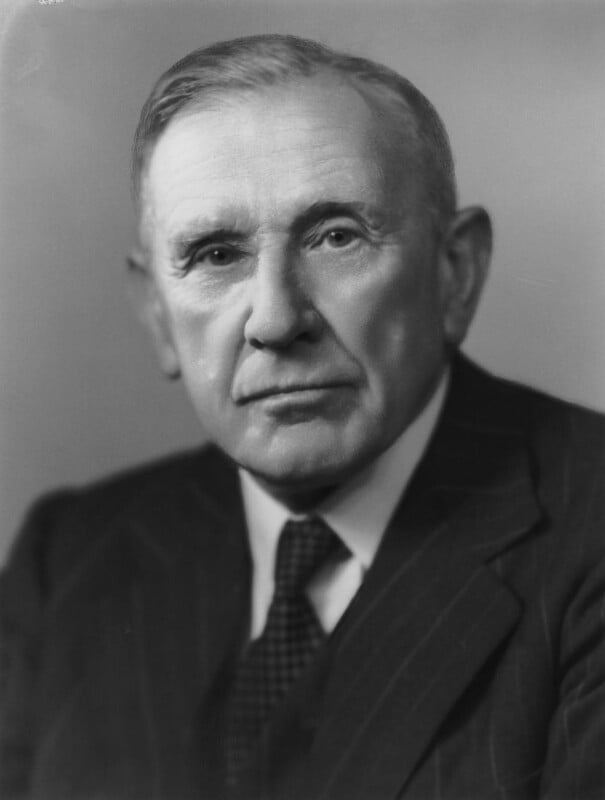
\includegraphics[height=0.42\textheight]{ch10_hurst_1953.jpg}\\[1mm]
\imgcap{Harold Edwin Hurst, 1953}
\imgcredit{https://commons.wikimedia.org/wiki/File:Harold_Edwin_Hurst_in_1953.jpg}{Photo: Elliott \& Fry (1953); public domain; Wikimedia Commons}
\end{column}
\begin{column}{0.62\textwidth}
\begin{itemize}
    \item Hurst studied centuries of Nile levels to size the reservoirs above Aswan \refHur
    \item The adjusted range of cumulated inflows grew like $n^H$ with $H \approx 0.7$, not $n^{1/2}$: the \textbf{Hurst effect}
    \item Wet years follow wet years in long runs: dependence that no finite ARMA reproduces
    \item Two explanations followed
    \begin{itemize}
        \item fractional Gaussian noise \refMVN
        \item fractional differencing \refGJ, \refHos
    \end{itemize}
\end{itemize}
\end{column}
\end{columns}
\end{frame}

\begin{frame}{Records of the river}
\itemsize{\small}
\begin{columns}[T]
\begin{column}{0.34\textwidth}
\centering
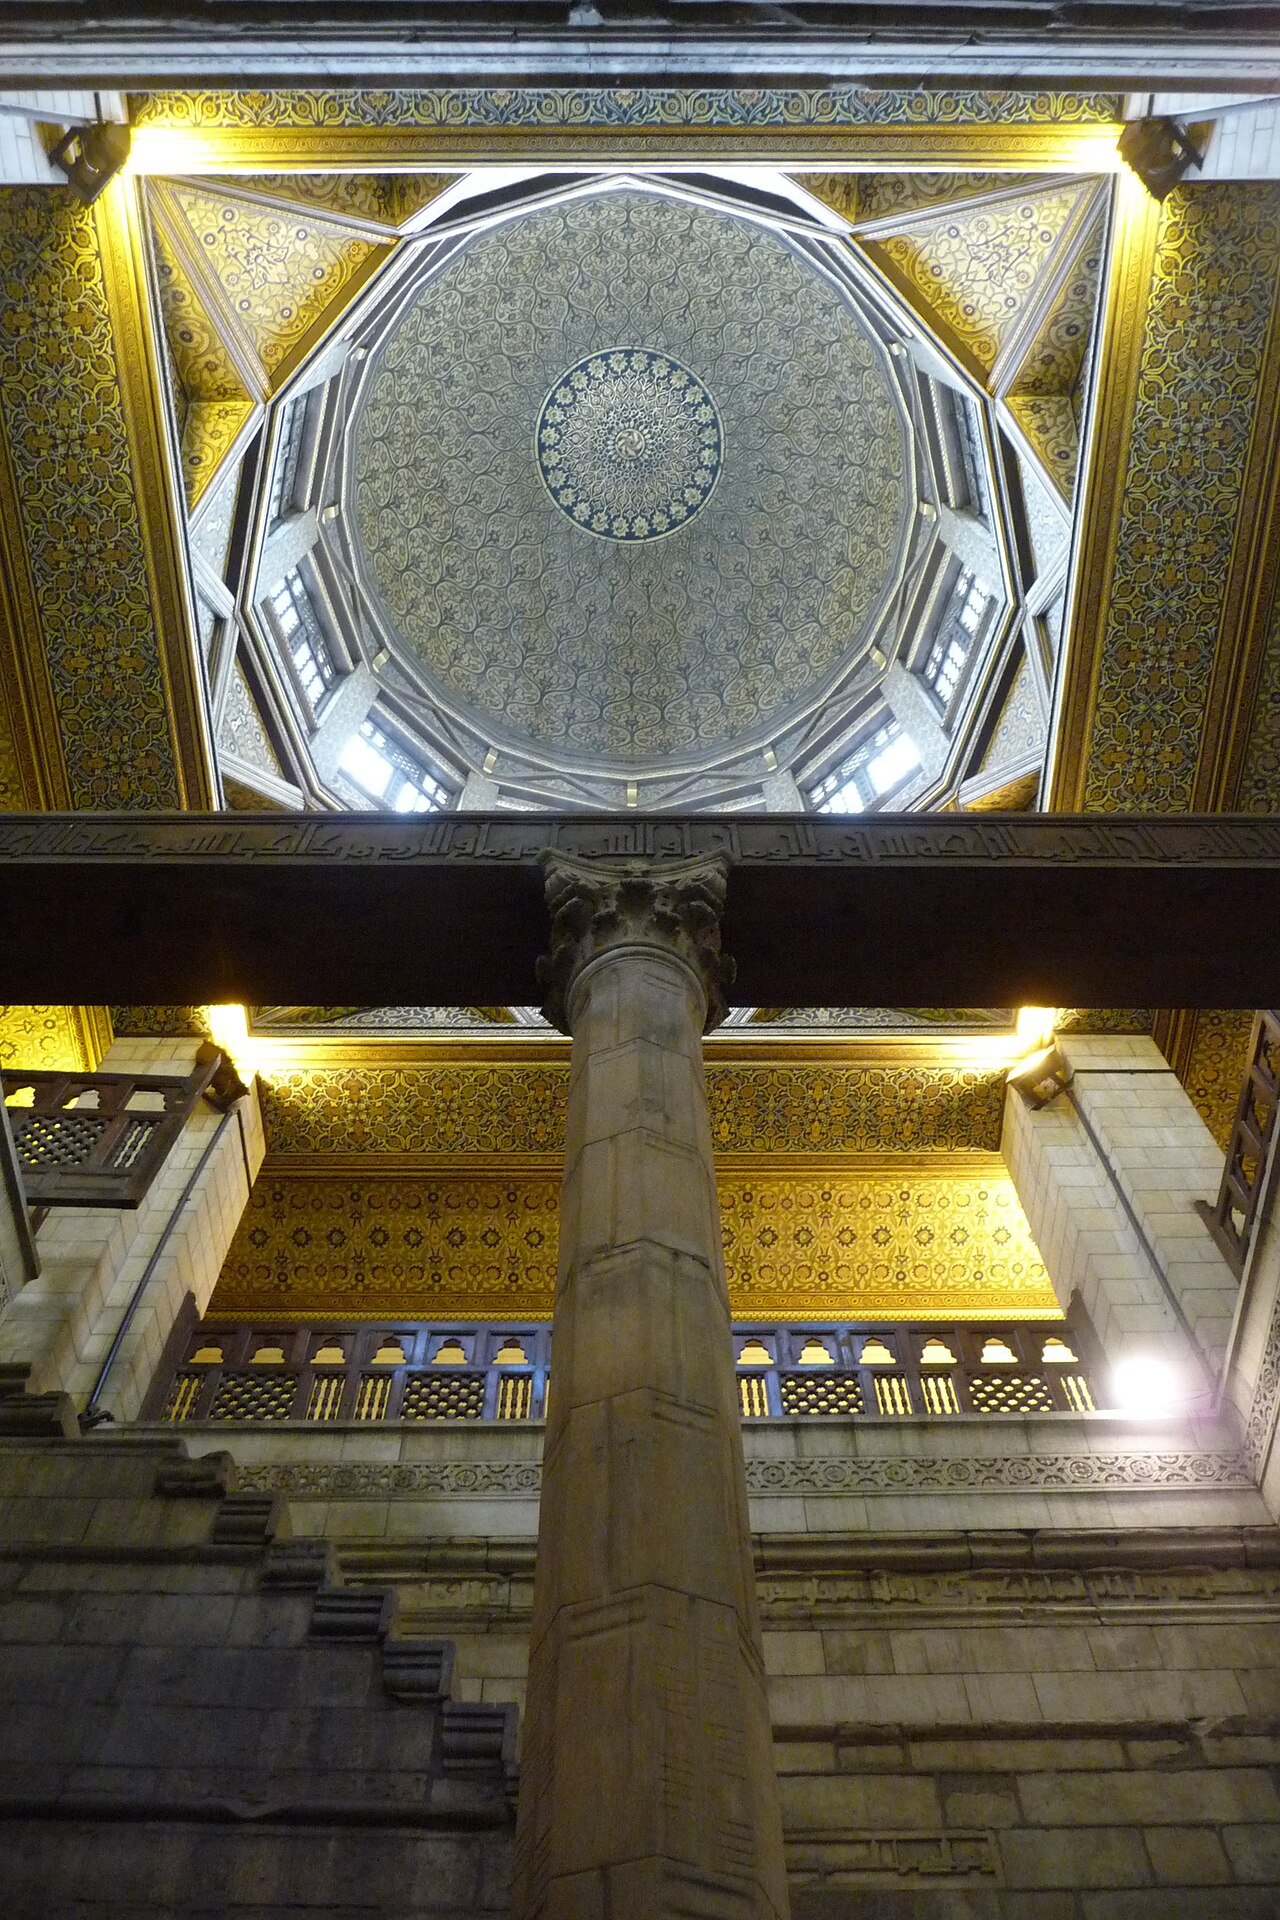
\includegraphics[height=0.5\textheight]{ch10_nilometer_2009.jpg}\\[1mm]
\imgcap{The Nilometer on Roda Island, Cairo}
\imgcredit{https://commons.wikimedia.org/wiki/File:Nilometer._Roda_Innen.JPG}{Photo: Willyman (2009); CC BY-SA 4.0; Wikimedia Commons}
\end{column}
\begin{column}{0.64\textwidth}
\begin{itemize}
    \item The Roda Nilometer recorded annual Nile minima from the seventh century on: one of the oldest time series
    \item These minima are the classic long-memory data set \refBFGK
    \item Today the same question is asked of volatility, inflation and interest rates: does a shock fade geometrically or hyperbolically?
    \item And a newer one: at short horizons, is volatility smoother or rougher than Brownian motion?
\end{itemize}
\end{column}
\end{columns}
\end{frame}

\begin{frame}{Twenty-two years of log realised variance}
\itemsize{\footnotesize}
\begin{center}
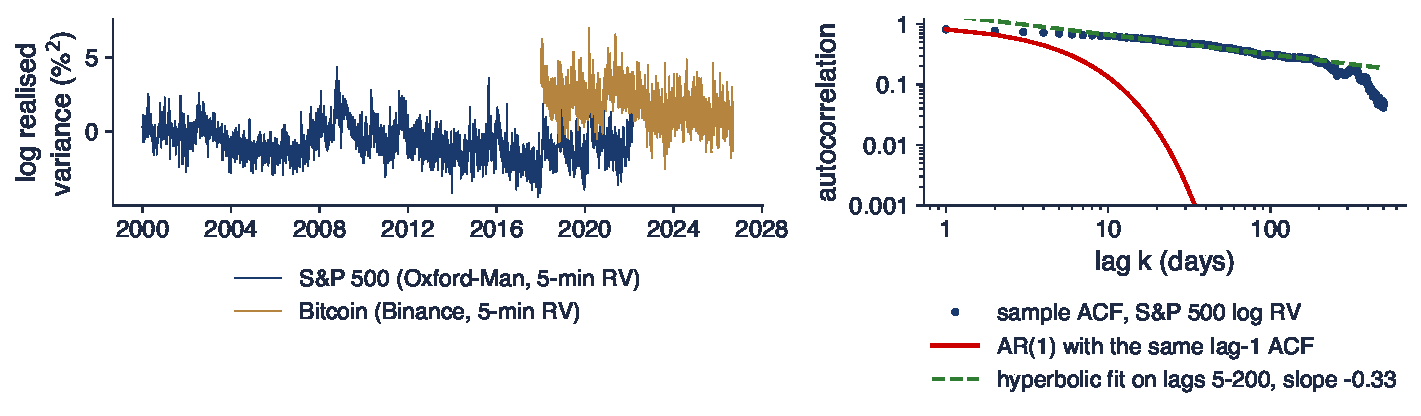
\includegraphics[width=0.97\textwidth,height=0.53\textheight,keepaspectratio]{ats_ch10_overview.pdf}
\end{center}
\vspace{-0.25cm}
\begin{itemize}
    \item Left: S\&P 500 (Oxford-Man, $n = 5\,552$ days to 25 February 2022) and Bitcoin ($n = 3\,165$ days to 18 September 2026); right: sample ACF of S\&P 500 log RV, lags 1--500, log-log
\end{itemize}
\quantlet{ATS\_ch10\_memory}{\qlurl{ATS_ch10_memory}}
\end{frame}

\begin{frame}{Interpreting the long view}
\itemsize{\small}
\begin{itemize}
    \item ACF 0.82 at lag 1, 0.53 at lag 22, still 0.18 at lag 250: an AR(1) with the same first lag would give about $10^{-22}$ at lag 250
    \item On lags 5--200 the ACF is a straight line in log-log, slope \ensuremath{-}0.33: hyperbolic decay $k^{2d-1}$ with $d \approx 0.34$
    \item The local Whittle estimate is larger, 0.62: the sample ACF is biased down at long lags under long memory
    \item The rest of the chapter asks which of these numbers to trust, and why the same series also looks rough
\end{itemize}
\end{frame}


%=============================================================================
\section{Long memory: spectral characterisation}
%=============================================================================

\begin{frame}{Known from TSA, and new here}
\itemsize{\small}
\begin{itemize}
    \item Known (\atschlink{https://danpele.github.io/Time-Series-Analysis/EN/Courses/chapter8_long_memory_arfima.pdf}{TSA, Chapter 8}): fractional differencing, ARFIMA$(p,d,q)$, R/S and DFA, GPH and local Whittle as recipes, FIGARCH and HAR in brief, spurious long memory by example
    \item New: the theory behind the recipes
    \begin{itemize}
        \item equivalent definitions, aggregation, the variance of the sample mean
        \item limit laws of the semiparametric estimators, non-stationary $d$, bias and the choice of $m$
        \item a formal test against level shifts; fractional cointegration; rough volatility
    \end{itemize}
    \item Replications: Granger (1980) aggregation, Qu (2011) design, Gatheral, Jaisson and Rosenbaum (2018, Section 2) scaling on the Oxford-Man data they used
\end{itemize}
\end{frame}

\begin{frame}{Two definitions of long memory (1/2)}
\itemsize{\small}
\begin{itemize}
    \item \textbf{Time domain}: the autocovariances decay hyperbolically and are not summable
    \[ \gamma(k) \sim c_\gamma\,k^{2d-1} \ \ (k \to \infty), \quad 0 < d < 1/2 \ \Rightarrow\ \sum_k|\gamma(k)| = \infty \]
    \begin{itemize}
        \item $\gamma(k)$: autocovariance at lag $k$; $d$: memory parameter; $c_\gamma > 0$: a constant; $a_k \sim b_k$ means $a_k/b_k \to 1$
        \item short memory: $\sum_k|\gamma(k)| < \infty$ (e.g.\ ARMA, with geometric decay)
    \end{itemize}
    \item \textbf{Frequency domain}: the spectral density has a pole at frequency zero
    \[ f(\lambda) \sim c_f\,\lambda^{-2d} \quad (\lambda \to 0^+) \]
    \begin{itemize}
        \item $f(\lambda)$: spectral density at frequency $\lambda \in (0, \pi]$; $c_f > 0$: a constant
        \item $d < 0$: antipersistence, $f(0) = 0$, $\sum_k\gamma(k) = 0$; $d = 0$: short memory
    \end{itemize}
\end{itemize}
\end{frame}

\begin{frame}{Two definitions of long memory (2/2)}
\itemsize{\small}
\begin{itemize}
    \item Equivalence: for quasi-monotone $\gamma$ the constants are linked (Abelian--Tauberian theorems) \refBFGK
    \[ c_f = c_\gamma\,\Gamma(2d)\,\frac{\sin(\pi/2 - \pi d)}{\pi} \]
    \begin{itemize}
        \item $\Gamma(\cdot)$: the gamma function; without such regularity the two definitions differ
        \item semiparametric estimators use only the frequency-domain definition
    \end{itemize}
    \item Hurst scale: $H = d + 1/2$ for the stationary series
    \begin{itemize}
        \item $H > 1/2$: persistent; $H < 1/2$: antipersistent; $H = 1/2$: short memory
    \end{itemize}
\end{itemize}
\end{frame}

\begin{frame}{Fractional integration and ARFIMA (1/2)}
\itemsize{\small}
\begin{itemize}
    \item The fractional difference operator is a power series in the lag operator $L$ ($LX_t = X_{t-1}$) \refGJ, \refHos
    \[ (1 - L)^d = \sum_{k\ge0}\pi_k L^k, \qquad \pi_0 = 1, \quad \pi_k = \pi_{k-1}\frac{k - 1 - d}{k}, \quad \pi_k \sim \frac{k^{-d-1}}{\Gamma(-d)} \]
    \begin{itemize}
        \item $\pi_k$: the weight of $X_{t-k}$; it decays hyperbolically, so the filter has infinite memory; $d = 1$ gives the usual difference $1 - L$
    \end{itemize}
    \item ARFIMA$(p,d,q)$: an ARMA for the fractionally differenced series
    \[ \phi(L)(1 - L)^d(X_t - \mu) = \theta(L)\varepsilon_t \]
    \begin{itemize}
        \item $\phi(L)$, $\theta(L)$: AR and MA polynomials of orders $p$, $q$; $\mu$: mean; $\varepsilon_t$: white noise with variance $\sigma^2$
        \item stationary and invertible for $-1/2 < d < 1/2$
    \end{itemize}
\end{itemize}
\end{frame}

\begin{frame}{Fractional integration and ARFIMA (2/2)}
\itemsize{\small}
\begin{itemize}
    \item Spectrum: a pole at zero times the spectrum of the ARMA part
    \[ f(\lambda) = \frac{\sigma^2}{2\pi}\,\big|2\sin(\lambda/2)\big|^{-2d}\,\frac{|\theta(e^{-i\lambda})|^2}{|\phi(e^{-i\lambda})|^2} = |2\sin(\lambda/2)|^{-2d}f^*(\lambda) \]
    \begin{itemize}
        \item $f^*$: the smooth short-memory (ARMA) part; near zero $|2\sin(\lambda/2)| \approx \lambda$, so $f(\lambda) \approx f^*(0)\lambda^{-2d}$
    \end{itemize}
    \item ARFIMA$(0,d,0)$: variance and autocorrelations in closed form
    \[ \gamma(0) = \sigma^2\frac{\Gamma(1 - 2d)}{\Gamma(1 - d)^2}, \qquad \rho(k) = \frac{\Gamma(k + d)\Gamma(1 - d)}{\Gamma(k - d + 1)\Gamma(d)} \sim \frac{\Gamma(1 - d)}{\Gamma(d)}k^{2d-1} \]
    \begin{itemize}
        \item recursion $\rho(k) = \rho(k - 1)\,(k - 1 + d)/(k - d)$, $\rho(1) = d/(1 - d)$
    \end{itemize}
\end{itemize}
\end{frame}

\begin{frame}{Hyperbolic and geometric decay}
\itemsize{\footnotesize}
\begin{center}
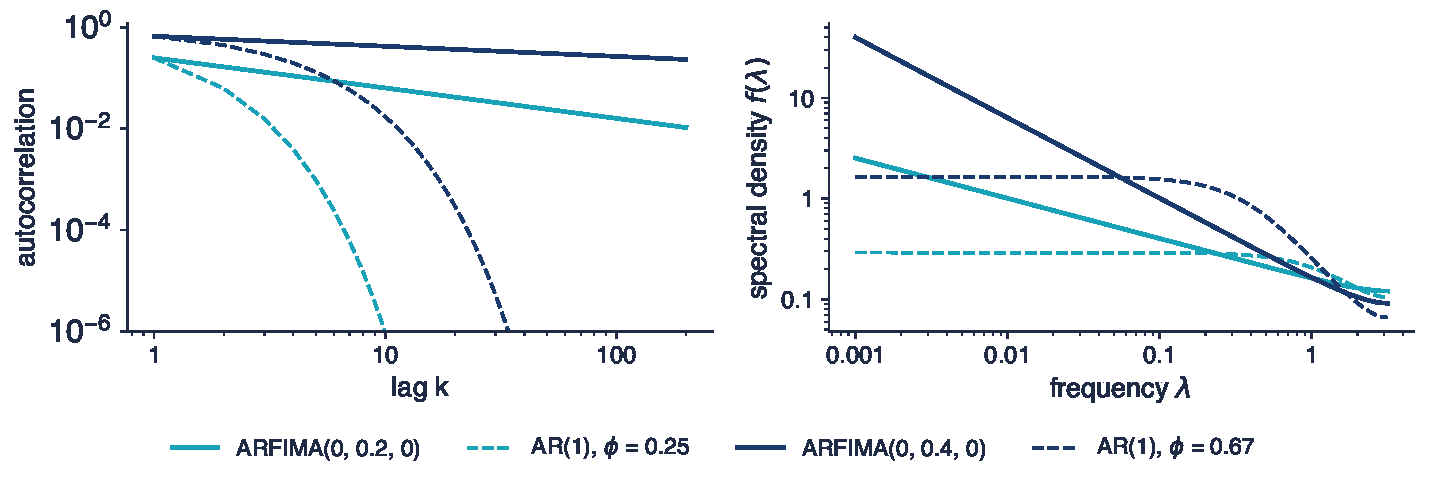
\includegraphics[width=0.97\textwidth,height=0.63\textheight,keepaspectratio]{ats_ch10_acf_spec.pdf}
\end{center}
\vspace{-0.25cm}
\begin{itemize}
    \item Left: ACF of ARFIMA$(0,d,0)$ and of an AR(1) with the same $\rho(1)$, log-log; right: spectral densities near zero, the AR(1) scaled to the same variance
\end{itemize}
\quantlet{ATS\_ch10\_memory}{\qlurl{ATS_ch10_memory}}
\end{frame}

\begin{frame}{Interpreting the two decays}
\itemsize{\small}
\begin{itemize}
    \item $d = 0.4$: $\rho(1) = 0.667$, $\rho(10) = 0.424$, $\rho(100) = 0.267$; the matching AR(1) has $\rho(100)$ of order $10^{-18}$
    \item Partial sums $\sum_{k\le100}\rho(k) = 33.0$ and $\sum_{k\le200}\rho(k) = 57.8$: they keep growing, like $K^{2d}$
    \item In the spectrum the difference is a pole against a plateau: long memory lives at the lowest frequencies, where few periodogram ordinates exist
    \item Hence all semiparametric estimators look only at the $m$ lowest Fourier frequencies
\end{itemize}
\end{frame}

\begin{frame}{Where long memory comes from: aggregation}
\itemsize{\small}
\begin{itemize}
    \item \refGra: the scaled sum of $N$ independent AR(1) series with random coefficients
    \[ X_t = \frac{1}{\sqrt N}\sum_{i=1}^N x_{it}, \qquad x_{it} = \phi_i x_{i,t-1} + \varepsilon_{it}, \qquad \phi_i^2 \sim \mathrm{Beta}(p, q) \]
    \begin{itemize}
        \item $\phi_i$: persistence of unit $i$, drawn once; Beta density $\propto \phi^{2p-1}(1 - \phi^2)^{q-1}$ on $(0, 1)$; $q$ controls the mass near the unit root
    \end{itemize}
    \item Derivation: average the AR(1) autocovariances over the distribution of $\phi$
    \[ \gamma_X(k) = \E\Big[\frac{\phi^k}{1 - \phi^2}\Big] \propto \int_0^1\phi^{k+2p-1}(1 - \phi^2)^{q-2}d\phi \propto B\Big(\frac{k}{2} + p, q - 1\Big) \sim c\,k^{-(q-1)} \]
    \begin{itemize}
        \item $B(\cdot, \cdot)$: the beta function; matching $k^{2d-1}$ gives $d = 1 - q/2$, long memory for $1 < q < 2$
    \end{itemize}
    \item Economic reading: aggregate inflation, volatility or output mixes many short-memory agents with heterogeneous persistence; a few near-unit-root units dominate the low frequencies
    \item Long memory can therefore be structural, not a curiosity of the estimator
\end{itemize}
\end{frame}

\begin{frame}{Aggregation of AR(1) series}
\itemsize{\footnotesize}
\begin{center}
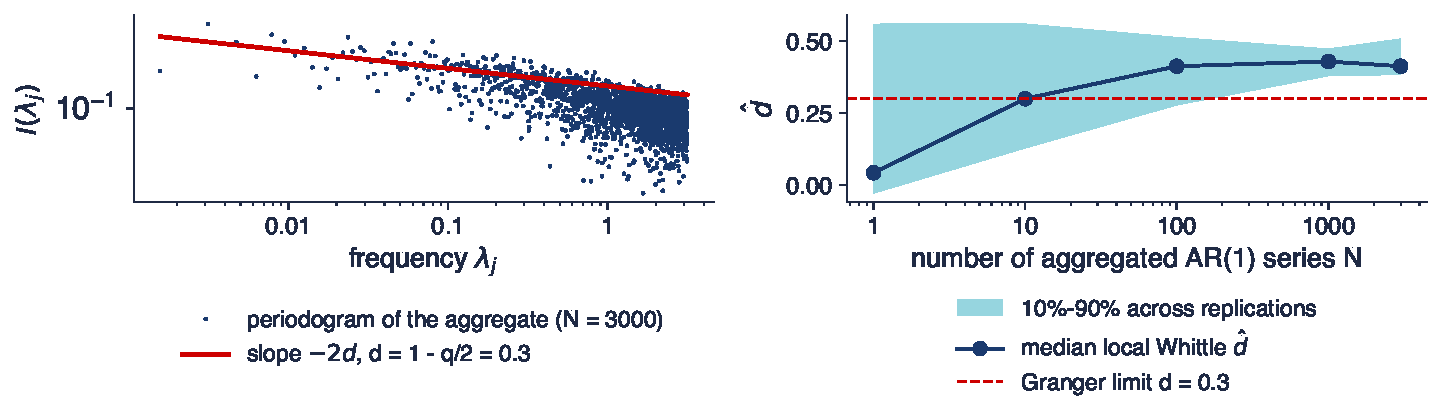
\includegraphics[width=0.97\textwidth,height=0.54\textheight,keepaspectratio]{ats_ch10_aggregation.pdf}
\end{center}
\vspace{-0.25cm}
\begin{itemize}
    \item $\phi_i^2 \sim \mathrm{Beta}(1, 1.4)$, so $d = 1 - q/2 = 0.3$; $n = 4000$; local Whittle with $m = 219$, 20 replications per $N$; left: periodogram of one aggregate of 3000 series
\end{itemize}
\quantlet{ATS\_ch10\_memory}{\qlurl{ATS_ch10_memory}}
\end{frame}

\begin{frame}{Interpreting aggregation}
\itemsize{\small}
\begin{itemize}
    \item One AR(1): median $\hat d = 0.04$; ten series: 0.30; 100 series: 0.41; 3000 series: 0.41 (10\%--90\%: 0.38 to 0.51)
    \item The estimate settles above the limit 0.3: the aggregate spectrum is $\lambda^{-2d}$ only very close to zero, and $m = n^{0.65}$ reaches into the region where it is not
    \item This is the bias problem of Section 2 in its purest form: a semiparametric estimator is only as good as its bandwidth
    \item The direction of the effect, from no memory to clear long memory, is the point of Granger's theorem
\end{itemize}
\end{frame}

\begin{frame}{Consequences for inference: the sample mean}
\itemsize{\small}
\begin{itemize}
    \item The variance of the sample mean $\bar X_n$ decays more slowly than $1/n$
    \[ \Var(\bar X_n) = \frac1n\sum_{|k|<n}\Big(1 - \frac{|k|}{n}\Big)\gamma(k) \sim \frac{c_\gamma}{d(2d + 1)}\,n^{2d-1} \]
    \begin{itemize}
        \item the mean converges at rate $n^{1/2-d}$, not $n^{1/2}$; with $d = 0.4$: $n^{0.1}$
    \end{itemize}
    \item HAC standard errors (\atschlink{https://danpele.github.io/Advanced-Time-Series/EN/Courses/chapter0_refresher_inference.pdf}{Chapter 0}) assume $\sum_k|\gamma(k)| < \infty$: under long memory the long-run variance is infinite and Newey--West intervals are too narrow
    \begin{itemize}
        \item the same holds for DM tests (\atschlink{https://danpele.github.io/Advanced-Time-Series/EN/Courses/chapter1_forecast_evaluation.pdf}{Chapter 1}) on loss differences that inherit long memory
    \end{itemize}
    \item Regression with long-memory regressors and errors: OLS slopes converge slowly
    \begin{itemize}
        \item spurious regression between independent fractional series when $d_x + d_u > 1/2$ ($d_x$, $d_u$: memory of the regressor and of the error)
    \end{itemize}
    \item Every test of this course built on $\sqrt n$ asymptotics needs a second look when $d > 0$
\end{itemize}
\end{frame}

\begin{frame}{Recap: Long memory}
\itemsize{\small}
\begin{itemize}
    \item Long memory: hyperbolic ACF $k^{2d-1}$ and a spectral pole $\lambda^{-2d}$; $H = d + 1/2$
    \item ARFIMA separates the pole $|2\sin(\lambda/2)|^{-2d}$ from the short-memory part $f^*$
    \item Aggregation of heterogeneous AR(1) units produces long memory; the mean converges at $n^{1/2-d}$
\end{itemize}
\end{frame}


%=============================================================================
\section{Semiparametric estimation and its asymptotics}
%=============================================================================

\begin{frame}{The periodogram near frequency zero}
\itemsize{\small}
\begin{itemize}
    \item The periodogram: the squared modulus of the discrete Fourier transform, at the Fourier frequencies
    \[ I(\lambda_j) = \frac{1}{2\pi n}\Big|\sum_{t=1}^n X_te^{-i\lambda_jt}\Big|^2, \qquad \lambda_j = \frac{2\pi j}{n}, \quad j = 1, \dots, m \]
    \begin{itemize}
        \item $n$: sample size; $m$: bandwidth, the number of lowest frequencies used; short memory: $I(\lambda_j)/f(\lambda_j)$ asymptotically i.i.d.\ $\mathrm{Exp}(1)$
    \end{itemize}
    \item Long memory: for fixed $j$, $\E\,I(\lambda_j)/f(\lambda_j) \not\to 1$ and the ordinates stay correlated \refRobB
    \begin{itemize}
        \item the distortion vanishes as $j \to \infty$: the proofs need $m \to \infty$, $m/n \to 0$, and handle the first frequencies separately
    \end{itemize}
    \item Semiparametric model: only the behaviour near zero is specified
    \[ f(\lambda) = G\lambda^{-2d}\big(1 + O(\lambda^\beta)\big), \qquad \lambda \to 0, \quad \beta \in (0, 2] \]
    \begin{itemize}
        \item $G > 0$: level of the spectrum at low frequencies; $\beta$: smoothness of the remainder; $\beta = 2$ for ARFIMA, because $f^*$ is smooth and even
    \end{itemize}
\end{itemize}
\end{frame}

\begin{frame}{GPH: the log-periodogram regression}
\itemsize{\small}
\begin{itemize}
    \item Taking logs of $I = f\xi$ gives a linear regression in $\log\lambda_j$ with slope $-2d$ \refGPH
    \[ \log I(\lambda_j) = \log G - 2d\log\lambda_j + \log\xi_j, \qquad \xi_j = \frac{I(\lambda_j)}{f(\lambda_j)} \]
    \begin{itemize}
        \item OLS on $j = 1, \dots, m$; with $\xi_j \sim \mathrm{Exp}(1)$: $\E\log\xi_j = -\gamma_E$ ($\gamma_E \approx 0.577$, Euler's constant), $\Var\log\xi_j = \pi^2/6$
    \end{itemize}
    \item \refRobB: for $|d| < 1/2$ and Gaussian $X$, if $m \to \infty$ and $m^5/n^4 \to 0$
    \[ \sqrt m(\hat d_{GPH} - d) \to N(0, \pi^2/24) \]
    \begin{itemize}
        \item origin of $\pi^2/24$: $\Var(\hat d) = \dfrac{\pi^2/6}{4\sum_j\nu_j^2}$, with $\nu_j = \log j - \overline{\log j}$ the centred regressor and $\sum_j\nu_j^2 \sim m$
    \end{itemize}
    \item Bias of order $(m/n)^2$ (formula on the bandwidth slide below)
    \begin{itemize}
        \item the condition $m^5/n^4 \to 0$ makes the bias negligible relative to the standard deviation $m^{-1/2}$
    \end{itemize}
\end{itemize}
\end{frame}

\begin{frame}{Local Whittle (1/2): the objective}
\itemsize{\small}
\begin{itemize}
    \item Whittle approximation of the Gaussian log-likelihood, restricted to $j \le m$, with $f(\lambda_j) = G\lambda_j^{-2d}$
    \[ Q(G, d) = \frac1m\sum_{j=1}^m\Big[\log\big(G\lambda_j^{-2d}\big) + \frac{I(\lambda_j)}{G\lambda_j^{-2d}}\Big] \]
    \begin{itemize}
        \item the same form as QLIKE (\atschlink{https://danpele.github.io/Advanced-Time-Series/EN/Courses/chapter8_advanced_volatility.pdf}{Chapter 8}): the model spectrum $G\lambda_j^{-2d}$ is fitted to the periodogram ordinate by ordinate
    \end{itemize}
    \item Concentrate out $G$ \refRobC: for given $d$ the optimal level is the average of $\lambda_j^{2d}I(\lambda_j)$
    \[ \hat G(d) = \frac1m\sum_j\lambda_j^{2d}I(\lambda_j), \qquad \hat d_{LW} = \arg\min_d R(d) \]
    \[ R(d) = \log\hat G(d) - \frac{2d}{m}\sum_{j=1}^m\log\lambda_j \]
    \begin{itemize}
        \item a one-dimensional minimisation in $d$
    \end{itemize}
\end{itemize}
\end{frame}

\begin{frame}{Local Whittle (2/2): the variance}
\itemsize{\small}
\begin{itemize}
    \item Score at the truth: a weighted sum of $\xi_j - 1$
    \[ R'(d) = \frac{2}{m}\sum_j\nu_j\Big(\frac{\lambda_j^{2d}I(\lambda_j)}{\hat G(d)} - 1\Big) \]
    \begin{itemize}
        \item $\nu_j = \log\lambda_j - \overline{\log\lambda}$: centred log frequency; with $\Var(\xi_j) = 1$ and $R''(d) \to 4$: $\sqrt m(\hat d - d) \to N(0, 4/16) = N(0, 1/4)$
    \end{itemize}
    \item No distributional assumption beyond a linear process with martingale-difference innovations
    \begin{itemize}
        \item efficiency relative to GPH: $(\pi^2/24)/(1/4) = \pi^2/6 \approx 1.64$
        \item derivation step by step: \atsapplink{atsapp1}{atssrc1}{Appendix}  % applink: the variance of local Whittle
    \end{itemize}
\end{itemize}
\end{frame}

\begin{frame}{Local Whittle: the theorem and its limits}
\itemsize{\small}
\begin{itemize}
    \item \refRobC: for $d \in (-1/2, 1/2)$, $f(\lambda) = G\lambda^{-2d}(1 + O(\lambda^\beta))$ and a bandwidth with $1/m + m^{1+2\beta}(\log m)^2/n^{2\beta} \to 0$
    \begin{itemize}
        \item $\hat d \to_p d$ and $\sqrt m(\hat d - d) \to N(0, 1/4)$; the condition on $m$: it grows, but slowly enough for the bias to vanish
    \end{itemize}
    \item Non-stationary $d$: consistent for $d < 1$, asymptotically Normal for $d < 3/4$ \refVel
    \begin{itemize}
        \item for $d > 1$ it converges in probability to 1; between $3/4$ and 1 the limit is non-Normal \refPS
    \end{itemize}
    \item Remedies: difference the data first (needs knowing $d > 1/2$), taper the periodogram (variance cost), or estimate exactly
\end{itemize}
\end{frame}

\begin{frame}{Exact local Whittle}
\itemsize{\small}
\begin{itemize}
    \item \refSP: replace $\lambda_j^{2d}I_X(\lambda_j)$ by the periodogram of the fractionally differenced data
    \[ \Delta^dX_t = \sum_{k=0}^{t-1}\pi_kX_{t-k}, \qquad R_E(d) = \log\Big(\frac1m\sum_jI_{\Delta^dX}(\lambda_j)\Big) - \frac{2d}{m}\sum_j\log\lambda_j \]
    \begin{itemize}
        \item $\Delta^d = (1 - L)^d$ truncated at the start of the sample; $I_{\Delta^dX}$: periodogram of the differenced series
        \item $\lambda^{2d}I_X(\lambda)$ approximates $I_{\Delta^dX}(\lambda)$ only for $d < 1/2$; the exact version removes the error that breaks LW for large $d$: $\sqrt m(\hat d_{ELW} - d) \to N(0, 1/4)$ on any search interval of width $< 9/2$
    \end{itemize}
    \item Unknown mean \refShi: subtract $\hat\mu(d) = w(d)\bar X + (1 - w(d))X_1$
    \begin{itemize}
        \item $w(d) = 1$ for $d \le 1/2$, $0$ for $d \ge 3/4$, smooth in between: the sample mean is a bad estimator of the level when $d > 1/2$
    \end{itemize}
    \item Cost: one fractional difference per evaluation, $O(n\log n)$ by FFT
\end{itemize}
\end{frame}

\begin{frame}{GPH, local Whittle and exact local Whittle by Monte Carlo}
\itemsize{\footnotesize}
\begin{center}
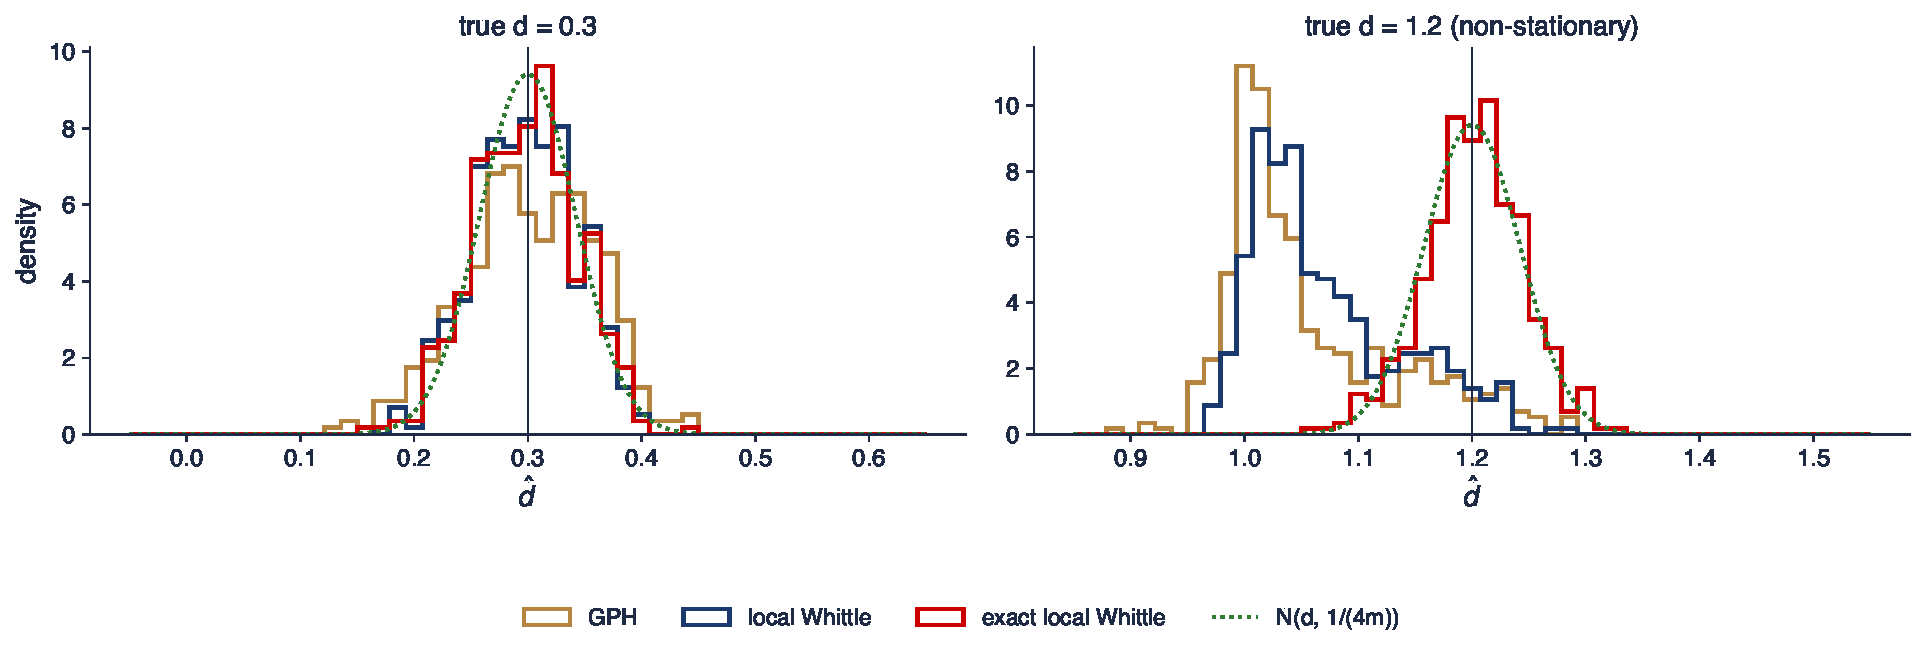
\includegraphics[width=0.97\textwidth,height=0.63\textheight,keepaspectratio]{ats_ch10_mc_estimators.pdf}
\end{center}
\vspace{-0.25cm}
\begin{itemize}
    \item 400 Gaussian ARFIMA$(0,d,0)$ paths, $n = 2000$, $m = n^{0.65} = 139$; asymptotic SD: GPH 0.054, local Whittle 0.042; $d = 1.2$ is simulated as the partial sum of an ARFIMA$(0, 0.2, 0)$
\end{itemize}
\quantlet{ATS\_ch10\_estimation}{\qlurl{ATS_ch10_estimation}}
\end{frame}

\begin{frame}{Interpreting the Monte Carlo}
\itemsize{\small}
\begin{itemize}
    \item $d = 0.3$: means 0.301, 0.297, 0.298; SD 0.057, 0.045, 0.045; 95\% coverage 94\%, 94\%, 95\% (GPH, LW, ELW)
    \item The asymptotic laws are accurate at $n = 2000$; local Whittle is about $\sqrt{\pi^2/6}$ times tighter than GPH
    \item $d = 1.2$: GPH 1.057 and LW 1.072 collapse towards 1 (coverage 26\% and 22\%); ELW 1.202, coverage 93\%
    \item For series that may be non-stationary (prices, inflation in levels, log RV with $d$ near 0.5) report ELW
\end{itemize}
\end{frame}

\begin{frame}{Bandwidth: bias against variance}
\itemsize{\small}
\begin{itemize}
    \item Leading bias (GPH and LW) \refHDB: the curvature of $\log f^*$ near zero leaks into the slope
    \[ \E\hat d - d \approx -\frac{2\pi^2}{9}\,\frac{f^{*\prime\prime}(0)}{f^*(0)}\Big(\frac mn\Big)^2 = C\Big(\frac mn\Big)^2 \]
    \begin{itemize}
        \item from regressing $\log f^*(\lambda_j) \approx \log f^*(0) + b\lambda_j^2$, $b = \tfrac12f^{*\prime\prime}(0)/f^*(0)$, on $-2\nu_j$; $C$: the bias constant
        \item ARFIMA$(1,d,0)$: $f^{*\prime\prime}(0)/f^*(0) = -2\phi/(1 - \phi)^2$, upward bias for $\phi > 0$
    \end{itemize}
    \item MSE: squared bias plus variance; minimising over $m$ gives the optimal bandwidth \refHR
    \[ \mathrm{MSE}(m) \approx C^2\Big(\frac mn\Big)^4 + \frac{1}{4m}, \qquad m^* = \Big(\frac{n^4}{16C^2}\Big)^{1/5} \propto n^{4/5} \]
    \begin{itemize}
        \item $C$ is unknown: plug-in rules estimate it; local polynomial Whittle \refAnSu\ removes the $\lambda^2$ term at a variance cost
    \end{itemize}
    \item At $m^*$ bias and SD are of the same order, so nominal intervals undercover; practice: plot $\hat d(m)$ over a range and report it with the intervals
\end{itemize}
\end{frame}

\begin{frame}{Bias and RMSE across bandwidths}
\itemsize{\footnotesize}
\begin{center}
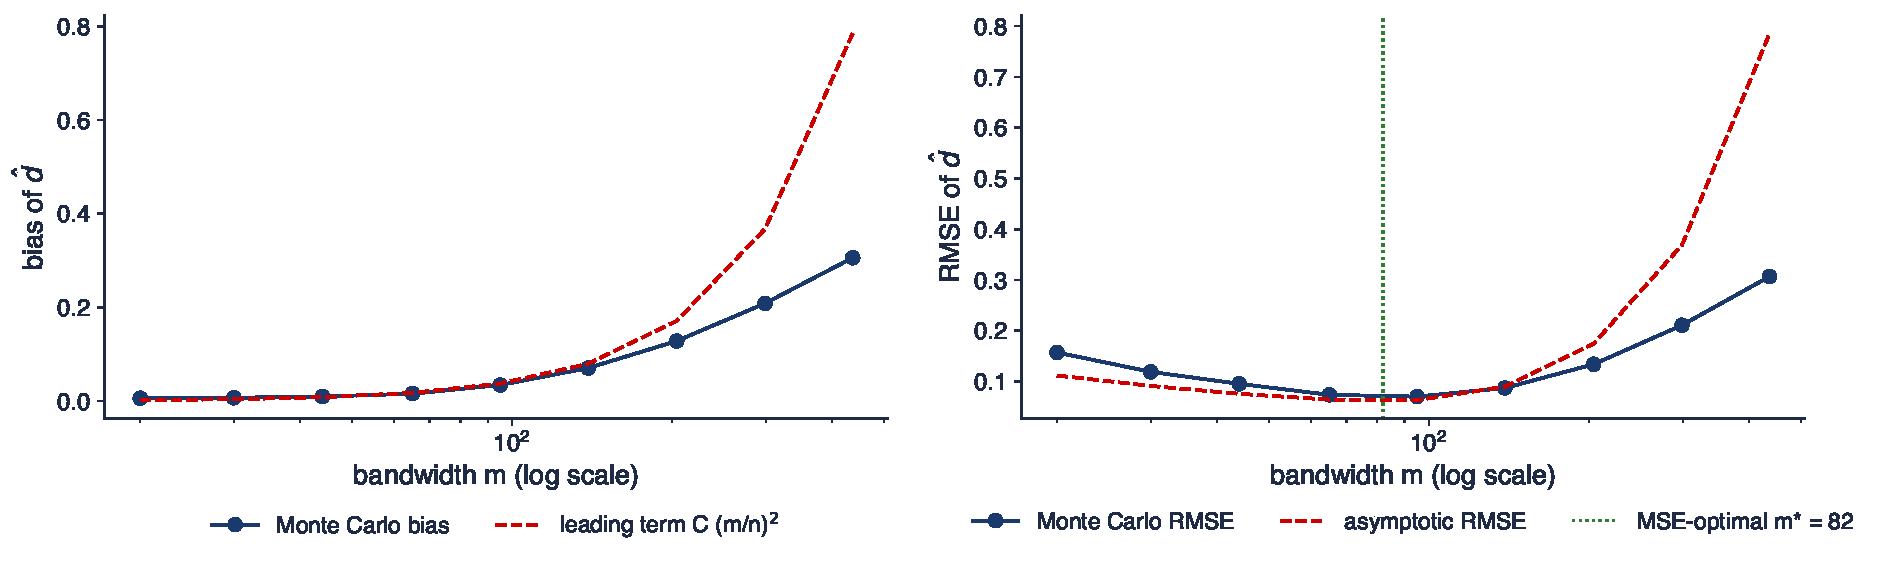
\includegraphics[width=0.97\textwidth,height=0.55\textheight,keepaspectratio]{ats_ch10_bandwidth.pdf}
\end{center}
\vspace{-0.25cm}
\begin{itemize}
    \item Local Whittle, ARFIMA$(1, 0.3, 0)$ with $\phi = 0.6$, $n = 2000$, 300 replications, $m = n^a$ for $a = 0.40, \dots, 0.80$; dashed: the leading bias $C(m/n)^2$ with $C = 16.4$ and the asymptotic RMSE
\end{itemize}
\quantlet{ATS\_ch10\_estimation}{\qlurl{ATS_ch10_estimation}}
\end{frame}

\begin{frame}{Interpreting the bandwidth trade-off}
\itemsize{\small}
\begin{itemize}
    \item Small $m$ ($a = 0.40$): bias 0.006, RMSE 0.16, dominated by variance; large $m$ ($a = 0.80$): bias 0.31, RMSE 0.31
    \item Smallest Monte Carlo RMSE 0.070 at $m = 95$ ($a = 0.60$); theory: $m^* = 82$ ($a = 0.58$)
    \item The leading term overstates the bias at large $m$ (0.79 against 0.31): the $\lambda^2$ expansion is local
    \item A fixed rule such as $m = n^{0.8}$ can turn a short-memory AR component into apparent long memory
\end{itemize}
\end{frame}

\begin{frame}{Parametric alternative: Whittle and exact ML}
\itemsize{\small}
\begin{itemize}
    \item Whittle: fit a fully specified spectral density over all frequencies \refFT
    \[ \hat\vartheta = \arg\min_\vartheta\sum_{j=1}^{\lfloor (n-1)/2\rfloor}\Big[\log f(\lambda_j; \vartheta) + \frac{I(\lambda_j)}{f(\lambda_j; \vartheta)}\Big] \]
    \begin{itemize}
        \item $\vartheta$: all ARFIMA$(p,d,q)$ parameters ($d$, the AR and MA coefficients, $\sigma^2$); $\sqrt n$-consistent and efficient if the model is right; $\Var(\hat d) \approx 6/(\pi^2n)$ for $(0,d,0)$
    \end{itemize}
    \item The trade-off is robustness against efficiency: a wrong $(p, q)$ biases $\hat d$ for every $n$
    \begin{itemize}
        \item semiparametric: rate $\sqrt m$, robust to $f^*$; parametric: rate $\sqrt n$, exposed to misspecification
    \end{itemize}
    \item Common practice: semiparametric $\hat d$ first, then a parametric model whose $d$ falls inside its interval, then forecasts
\end{itemize}
\end{frame}

\begin{frame}{Recap: Semiparametric estimation}
\itemsize{\small}
\begin{itemize}
    \item GPH: $N(d, \pi^2/(24m))$; local Whittle: $N(d, 1/(4m))$; exact local Whittle keeps $N(d, 1/(4m))$ for non-stationary $d$
    \item Bias $\propto (m/n)^2$, SD $\propto m^{-1/2}$: MSE-optimal $m \propto n^{4/5}$, with an unknown constant
    \item Always report $\hat d(m)$ across bandwidths
\end{itemize}
\end{frame}


%=============================================================================
\section{Short or long memory: testing against level shifts}
%=============================================================================

\begin{frame}{Mechanisms of spurious long memory}
\itemsize{\small}
\begin{itemize}
    \item \refDI: Markov switching in the mean with switching probability $p_n \to 0$ as $n \to \infty$ produces $\Var(\sum_{t\le n}X_t) = O(n^{2d+1})$, like an I($d$) process
    \begin{itemize}
        \item rare breaks are invisible at high frequencies and look like a pole at low ones \refGH
    \end{itemize}
    \item Random level shifts \refLP: a short-memory series $u_t$ around a level that jumps rarely
    \[ X_t = \mu_t + u_t, \qquad \mu_t = \mu_{t-1} + \delta_t\eta_t, \qquad \delta_t \sim \mathrm{Bernoulli}(p) \]
    \begin{itemize}
        \item $\delta_t$: 1 on the (rare) days with a shift; $\eta_t$: shift size, variance $\sigma^2_\eta$; spectrum $\approx p\sigma_\eta^2/(2\pi\lambda^2)$ above frequency $\approx p$, plus the flat $f_u$: a slope $-2$ that fades into a plateau
    \end{itemize}
    \item Signature \refPQ: under level shifts $\hat d(m)$ falls steeply as $m$ grows; under true long memory it is flat
    \begin{itemize}
        \item the same reasoning applies to trends, regime switches and deterministic seasonality left in the data
    \end{itemize}
    \item \atschlink{https://danpele.github.io/Time-Series-Analysis/EN/Courses/chapter8_long_memory_arfima.pdf}{TSA, Chapter 8} showed the phenomenon by example; here: a formal test with known size
\end{itemize}
\end{frame}

\begin{frame}{The Qu (2011) test}
\itemsize{\small}
\begin{itemize}
    \item Under $H_0$ (stationary long memory) the LW score has mean zero in every frequency band; under level shifts the low frequencies are over-weighted \refQu
    \[ W = \sup_{r\in[\varepsilon, 1]}\Big(\sum_{j=1}^m\nu_j^2\Big)^{-1/2}\Big|\sum_{j=1}^{\lfloor mr\rfloor}\nu_j\Big(\frac{I(\lambda_j)}{\hat G\lambda_j^{-2\hat d}} - 1\Big)\Big| \]
    \begin{itemize}
        \item $\hat d, \hat G$: local Whittle on the same $m$; $\nu_j = \log\lambda_j - \overline{\log\lambda}$; $r$: the share of the $m$ frequencies included; $\varepsilon$: trimming of the lowest band
        \item the partial sum at $r = 1$ is zero by the first-order condition; $W$: the largest standardised partial sum
    \end{itemize}
    \item Limit: the supremum of a Gaussian process free of $d$ and $G$; Qu recommends $m = n^{0.7}$, $\varepsilon = 0.02$ (large $n$) or $0.05$
    \begin{itemize}
        \item our simulated critical values: $\varepsilon = 0.02$: 1.09, 1.22, 1.56; $\varepsilon = 0.05$: 1.00, 1.14, 1.45 (10\%, 5\%, 1\%)
        \item reject for large $W$: evidence against stationary long memory, typically breaks, level shifts or trends
    \end{itemize}
\end{itemize}
\end{frame}

\begin{frame}{Size, power and the bandwidth signature}
\itemsize{\footnotesize}
\begin{center}
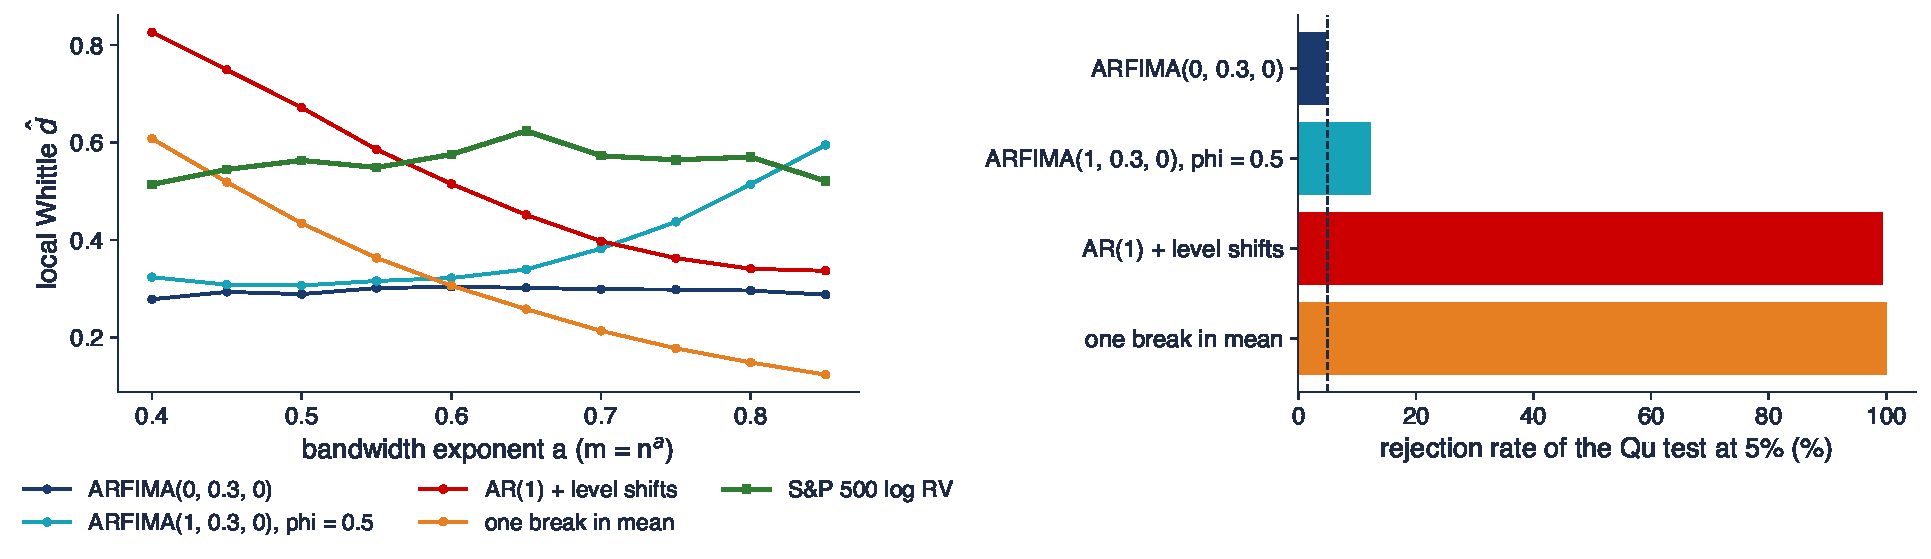
\includegraphics[width=0.97\textwidth,height=0.54\textheight,keepaspectratio]{ats_ch10_qu.pdf}
\end{center}
\vspace{-0.25cm}
\begin{itemize}
    \item $n = 2000$, 300 replications, $m = n^{0.7} = 204$, $\varepsilon = 0.02$; left: mean local Whittle $\hat d(m)$ (100 paths) and the S\&P 500 log RV; right: rejection rates at 5\%
\end{itemize}
\quantlet{ATS\_ch10\_qu\_test}{\qlurl{ATS_ch10_qu_test}}
\end{frame}

\begin{frame}{Interpreting the Qu test}
\itemsize{\small}
\begin{itemize}
    \item Size: 5\% under ARFIMA$(0, 0.3, 0)$, 12\% when an AR(1) with $\phi = 0.5$ is added: short-run dynamics distort size in finite samples
    \item Power: 99\% against level shifts and 100\% against one break, although LW reports $\hat d = 0.39$ and 0.21
    \item Signature: under level shifts $\hat d(m)$ drops from 0.83 to 0.34; S\&P 500 log RV stays between 0.51 and 0.62, and $W = 0.66$ is far below the 10\% value
    \item The memory of realised variance survives this test; Section 5 shows that $|r_t|$ of the BET and EUR/RON does not
\end{itemize}
\end{frame}

\begin{frame}{Inflation persistence and the disinflation}
\itemsize{\footnotesize}
\begin{center}
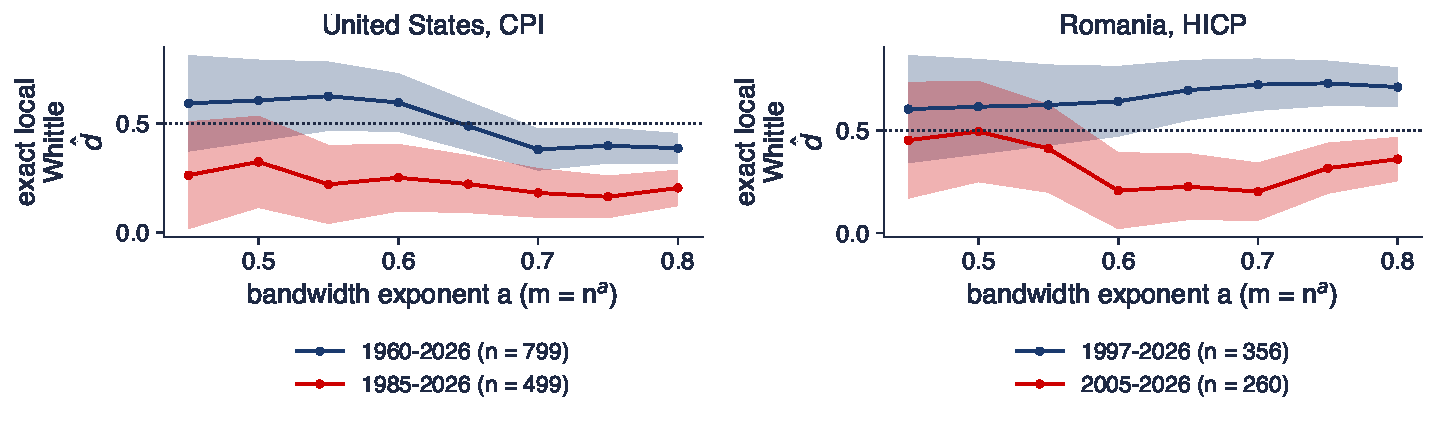
\includegraphics[width=0.97\textwidth,height=0.54\textheight,keepaspectratio]{ats_ch10_inflation.pdf}
\end{center}
\vspace{-0.25cm}
\begin{itemize}
    \item Monthly inflation, \% annualised: US CPI (seasonally adjusted) to August 2026, Romanian HICP (monthly means removed) to August 2026; exact local Whittle with unknown mean, 95\% bands; full sample and after the disinflation (US from 1985, Romania from 2005)
\end{itemize}
\quantlet{ATS\_ch10\_qu\_test}{\qlurl{ATS_ch10_qu_test}}
\end{frame}

\begin{frame}{Interpreting inflation persistence}
\itemsize{\small}
\begin{itemize}
    \item US: $\hat d = 0.49$ (SE 0.06) on 1960--2026 but 0.22 after 1985; Qu $W = 1.62$ (1\% value 1.45) rejects for the full sample, $W = 0.55$ after 1985
    \item Romania: $\hat d = 0.70$ with the 1997--2004 disinflation, 0.23 from 2005 (range 0.20 to 0.50 across bandwidths); $W = 0.86$ and 1.04 with only 356 and 260 months
    \item Plain local Whittle on the full Romanian sample gives 0.31: with a trend-like level shift only the exact version with the Shimotsu mean is reliable
    \item Within a stable monetary regime inflation keeps moderate long memory, $\hat d$ = 0.22 and 0.23 \refHW, \refBCT; the large estimates belong to regime changes
\end{itemize}
\end{frame}

\begin{frame}{Recap: Short or long memory}
\itemsize{\small}
\begin{itemize}
    \item Breaks, level shifts and rare regime switches create a spectral pole and a large $\hat d$
    \item Diagnostic: $\hat d(m)$ falling with $m$; test: Qu (2011), with simulated critical values
    \item US inflation: long memory is mostly the Great Inflation; log RV passes the test
\end{itemize}
\end{frame}


%=============================================================================
\section{Fractional cointegration}
%=============================================================================

\begin{frame}{Fractional cointegration and the FCVAR (1/2)}
\itemsize{\small}
\begin{itemize}
    \item $X_t \in \mathbb R^p$ is I($d$); it is \textbf{fractionally cointegrated} if $\beta'X_t$ is I($d - b$), $b > 0$
    \begin{itemize}
        \item $d$: memory of the series; $b$: reduction of memory achieved by the combination $\beta'X_t$; \atschlink{https://danpele.github.io/Advanced-Time-Series/EN/Courses/chapter4_cointegration_vecm_ardl_panel.pdf}{Chapter 4} is the case $d = b = 1$
    \end{itemize}
    \item FCVAR \refJN: the VECM with the difference $\Delta$ replaced by fractional differences
    \[ \Delta^dX_t = \alpha\beta'L_b\Delta^{d-b}X_t + \sum_{i=1}^k\Gamma_i\Delta^dL_b^iX_t + \varepsilon_t, \qquad L_b = 1 - \Delta^b \]
    \begin{itemize}
        \item $\Delta^d = (1 - L)^d$; $L_b$: fractional lag operator ($L_1 = L$), so $d = b = 1$ gives the VECM
        \item $\alpha$ ($p \times r$): adjustment; $\beta$ ($p \times r$): cointegrating vectors, rank $r$; $\Gamma_i$: short-run matrices, $k$ lags; $\varepsilon_t$: i.i.d. errors
    \end{itemize}
\end{itemize}
\end{frame}

\begin{frame}{Fractional cointegration and the FCVAR (2/2): estimation and rank}
\itemsize{\small}
\begin{itemize}
    \item For fixed $(d, b)$: a reduced-rank regression of $Z_0 = \Delta^dX$ on $Z_1 = L_b\Delta^{d-b}X$; then profile the likelihood over $(d, b)$
    \[ \ell_r(d, b) = -\frac T2\Big[\log\det S_{00} + \sum_{i\le r}\log(1 - \hat\lambda_i)\Big] \]
    \begin{itemize}
        \item $S_{00}$: residual covariance of $Z_0$ (after the short-run terms); $\hat\lambda_i$: the Johansen eigenvalues, in decreasing order; $T$: sample size
    \end{itemize}
    \item Rank tests: the LR trace statistic for rank $r$ against $p$
    \begin{itemize}
        \item for $b < 1/2$ it is asymptotically $\chi^2_{(p-r)^2}$; for $b > 1/2$ use the fractional Dickey--Fuller distributions of \refMN
    \end{itemize}
\end{itemize}
\end{frame}

\begin{frame}{Semiparametric co-memory}
\itemsize{\small}
\begin{itemize}
    \item Narrow-band least squares (NBLS) \refRobA, \refCN: regress $y$ on $x$ using only the $m$ lowest frequencies
    \[ \hat\beta = \frac{\mathrm{Re}\sum_{j=1}^mI_{xy}(\lambda_j)}{\sum_{j=1}^mI_{xx}(\lambda_j)} \]
    \begin{itemize}
        \item $I_{xy}$: cross-periodogram of $x$ and $y$; $I_{xx}$: periodogram of $x$; $\mathrm{Re}$: real part
        \item only the low frequencies, where the common long-memory component lives: robust to short-run correlation between $x$ and the error that biases OLS
    \end{itemize}
    \item Rank by ELW \refNS: estimate $d$ of each series, test equal $d$, then count the small eigenvalues of the low-frequency spectral matrix
    \item Implied and realised variance \refBP: does the VIX contain the long-memory component of future realised variance?
    \begin{itemize}
        \item if $\log RV$ and $\log VIX^2$ share one fractional trend, a combination has lower $d$ and the VIX forecasts the persistent part
    \end{itemize}
\end{itemize}
\end{frame}

\begin{frame}{FCVAR: realised and implied variance}
\itemsize{\footnotesize}
\begin{center}
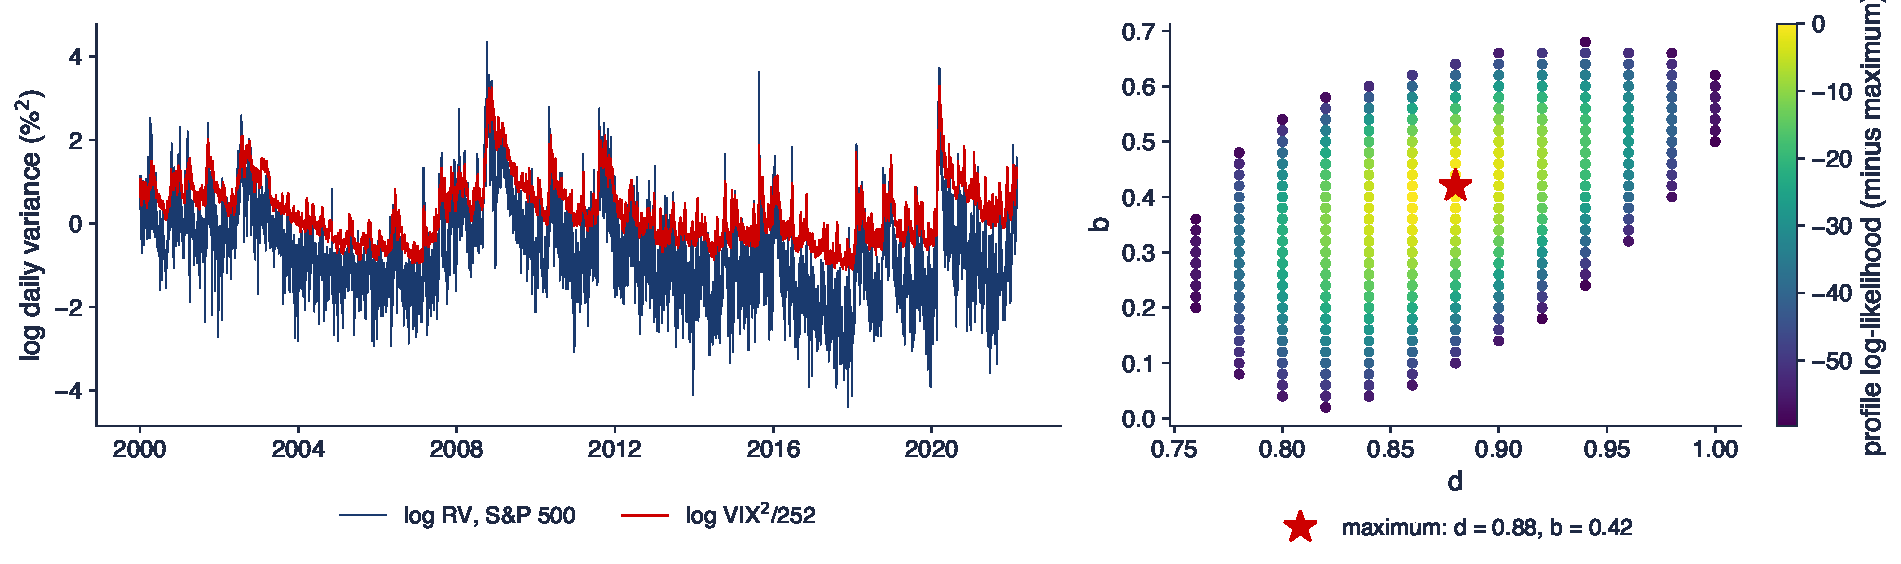
\includegraphics[width=0.97\textwidth,height=0.55\textheight,keepaspectratio]{ats_ch10_fcvar.pdf}
\end{center}
\vspace{-0.25cm}
\begin{itemize}
    \item S\&P 500 log 5-minute RV and $\log(\mathrm{VIX}^2/252)$, $n = 5\,523$ common days to 25 February 2022; right: profile log-likelihood of the rank-one FCVAR with $k = 0$ over $(d, b)$, the 60 log-points below the maximum
\end{itemize}
\quantlet{ATS\_ch10\_fcvar}{\qlurl{ATS_ch10_fcvar}}
\end{frame}

\begin{frame}{Interpreting the FCVAR}
\itemsize{\small}
\begin{itemize}
    \item Local Whittle: $d$ = 0.62 for log RV, 0.83 for log VIX$^2$, 0.49 for the spread $\beta'X_t$ (SE 0.03): the combination is less persistent
    \item FCVAR: $\hat d = 0.88$, $\hat b = 0.42$, $\beta = (1, -1.70)$, $\alpha = (\ensuremath{-}1.55, 0.006)$: realised variance adjusts, the VIX does not (weak exogeneity)
    \item Trace tests ($\hat b < 1/2$, so $\chi^2$): rank 0 against 2: 1453.94 ($p$ $<$0.001); rank 1 against 2: 18.26 ($p$ $<$0.001): with $k = 0$ the data also reject a single relation
    \item NBLS slope of log RV on log VIX$^2$: 1.27, against $1/1.70 = 0.59$ implied by FCVAR: short-run dynamics ($k > 0$) and the overnight gap of RV are left out; a project question
\end{itemize}
\end{frame}

\begin{frame}{Recap: Fractional cointegration}
\itemsize{\small}
\begin{itemize}
    \item FCVAR generalises the VECM with two memory parameters $d$ and $b$, estimated by profile likelihood and reduced-rank regression
    \item Rank tests are $\chi^2$ only for $b < 1/2$; NBLS and ELW give semiparametric checks
    \item Realised and implied variance share persistent components; the exact structure needs short-run dynamics
\end{itemize}
\end{frame}


%=============================================================================
\section{Long memory in volatility}
%=============================================================================

\begin{frame}{FIGARCH (1/2): hyperbolic ARCH weights}
\itemsize{\small}
\begin{itemize}
    \item GARCH(1,1) as ARCH($\infty$): the weights on past squared shocks decay geometrically
    \[ \sigma_t^2 = \frac{\omega}{1 - \beta} + \sum_{k\ge1}\alpha\beta^{k-1}\varepsilon_{t-k}^2 \]
    \item FIGARCH(1,$d$,1) \refBBM: a fractional difference makes them decay hyperbolically
    \[ \sigma_t^2 = \frac{\omega}{1 - \beta} + \Big[1 - \frac{(1 - \phi L)(1 - L)^d}{1 - \beta L}\Big]\varepsilon_t^2 = \frac{\omega}{1 - \beta} + \sum_{k\ge1}\lambda_k\varepsilon_{t-k}^2 \]
    \begin{itemize}
        \item $d \in (0, 1)$: memory of volatility; $\phi$, $\beta$: short-run ARCH and GARCH terms; $\lambda_k \sim c\,k^{-d-1}$: the ARCH($\infty$) weights
        \item positivity of all $\lambda_k$ needs restrictions, e.g.\ $\beta - d \le \phi \le (2 - d)/3$
    \end{itemize}
\end{itemize}
\end{frame}

\begin{frame}{FIGARCH (2/2): the variance paradox and HYGARCH}
\itemsize{\small}
\begin{itemize}
    \item Paradox: $\sum_k\lambda_k = 1$, so $\E\varepsilon_t^2 = \infty$
    \begin{itemize}
        \item FIGARCH is not covariance stationary for any $d > 0$, yet strictly stationary
        \item the long memory of $\varepsilon_t^2$ is therefore not defined by an autocovariance
    \end{itemize}
    \item HYGARCH \refDav: $(1 - L)^d$ is replaced by $1 + a\big((1 - L)^d - 1\big)$
    \begin{itemize}
        \item $a \ge 0$: amplitude of the hyperbolic part; $a < 1$ gives a finite variance and hyperbolic memory, $a = 1$ is FIGARCH, $a = 0$ is GARCH
    \end{itemize}
\end{itemize}
\end{frame}

\begin{frame}{ARCH weights: geometric and hyperbolic}
\itemsize{\footnotesize}
\begin{center}
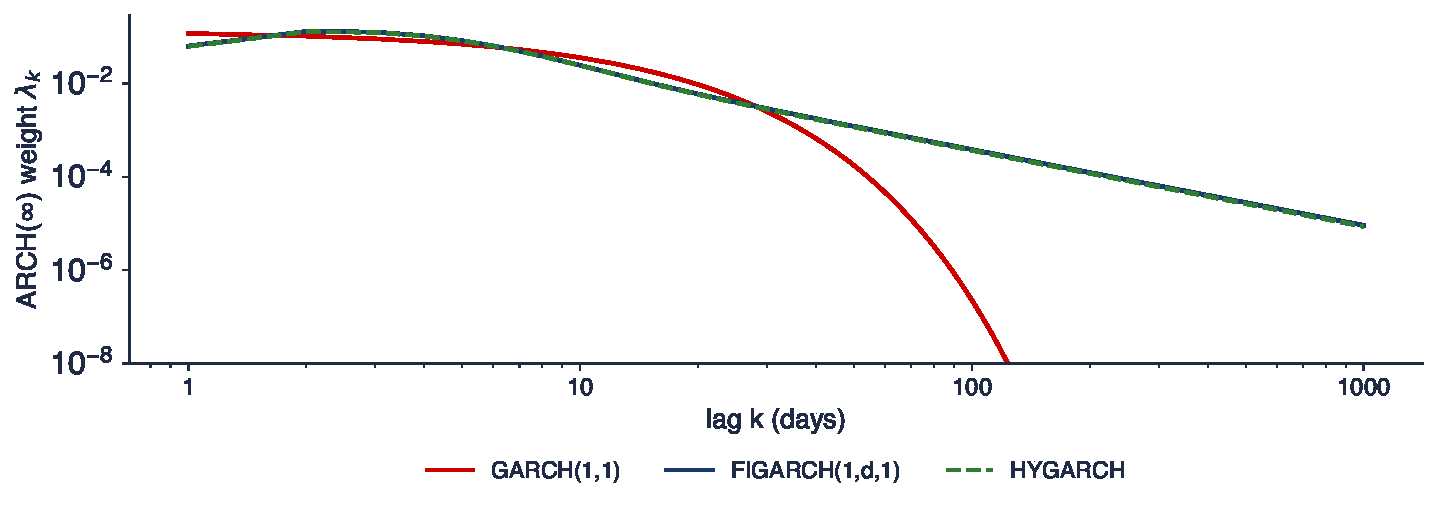
\includegraphics[width=0.97\textwidth,height=0.65\textheight,keepaspectratio]{ats_ch10_figarch.pdf}
\end{center}
\vspace{-0.25cm}
\begin{itemize}
    \item S\&P 500 daily returns 2000--2026 ($n = 6\,714$), Student $t$ QML, ARCH($\infty$) truncated at 1000 lags; GARCH $(\alpha, \beta) = (0.119, 0.876)$, FIGARCH $d = 0.61$, $\phi = 0.04$, $\beta = 0.59$
\end{itemize}
\quantlet{ATS\_ch10\_figarch}{\qlurl{ATS_ch10_figarch}}
\end{frame}

\begin{frame}{Interpreting the FIGARCH estimates}
\itemsize{\footnotesize}
\begin{center}
\scriptsize
\begin{tabular}{lcccccc}
\toprule
\textbf{Market} & $\hat d$ & LR & $\hat a$ & BIC GARCH & BIC FIGARCH & weight after lag 22 \\
\midrule
S\&P 500 & 0.61 & 40.8 & 0.99 & 18197 & 18165 & 15\% / 5\% \\
BET & 0.46 & 79.0 & 1.00 & 19514 & 19444 & 17\% / 1\% \\
Bitcoin & 0.98 & 13.6 & 1.06 & 20942 & 20936 & 12\% / 8\% \\
\bottomrule
\end{tabular}
\end{center}
\begin{itemize}
    \item LR of FIGARCH against GARCH (one more parameter): 40.8, 79.0, 13.6; BIC prefers FIGARCH in all three markets
    \item Weight on squared shocks older than 22 days: FIGARCH 15\%, GARCH 5\% (S\&P 500); after 250 days 2.0\% against practically zero
    \item HYGARCH amplitude $\hat a$ = 0.99 and 1.00: no evidence against $a = 1$ (LR 0.22 and 0.01); Bitcoin $\hat d = 0.98$ sits at the integrated edge
    \item LR: likelihood-ratio statistic of FIGARCH against GARCH; $\hat a$: HYGARCH amplitude; last column: FIGARCH / GARCH
\end{itemize}
\end{frame}

\begin{frame}{Long-memory stochastic volatility and noise}
\itemsize{\small}
\begin{itemize}
    \item LMSV \refBCL: log variance is a long-memory process; squaring and taking logs makes the model linear
    \[ r_t = \sigma_t\eta_t, \quad \log\sigma_t^2 = \mu + h_t \ \Rightarrow\ \log r_t^2 = \mu + \E\log\eta^2 + h_t + \xi_t \]
    \begin{itemize}
        \item $h_t$: ARFIMA$(p,d,q)$; $\eta_t$: i.i.d. shock; $\xi_t = \log\eta_t^2 - \E\log\eta^2$: i.i.d.\ noise with variance $\pi^2/2$ for Gaussian $\eta$, often larger than $\Var(h_t)$
    \end{itemize}
    \item Spectrum of $\log r_t^2$: a pole plus a flat noise floor
    \[ f(\lambda) = G\lambda^{-2d} + \frac{\sigma_\xi^2}{2\pi} \]
    \begin{itemize}
        \item the flat noise flattens the low-frequency slope and biases $\hat d$ down
        \item LW with noise \refHMS: $f(\lambda) = G(\lambda^{-2d} + \theta)$, with the noise-to-signal ratio $\theta \ge 0$ estimated jointly; consistent, at a slower rate
    \end{itemize}
    \item Realised variance reduces the noise by averaging intraday returns \refABDL: $\log RV_t = \log IV_t + $ small error
    \item Continuous-time long memory in volatility: \refCR; the rough alternative follows in Section 6
\end{itemize}
\end{frame}

\begin{frame}{Memory of volatility proxies across markets}
\itemsize{\footnotesize}
\begin{center}
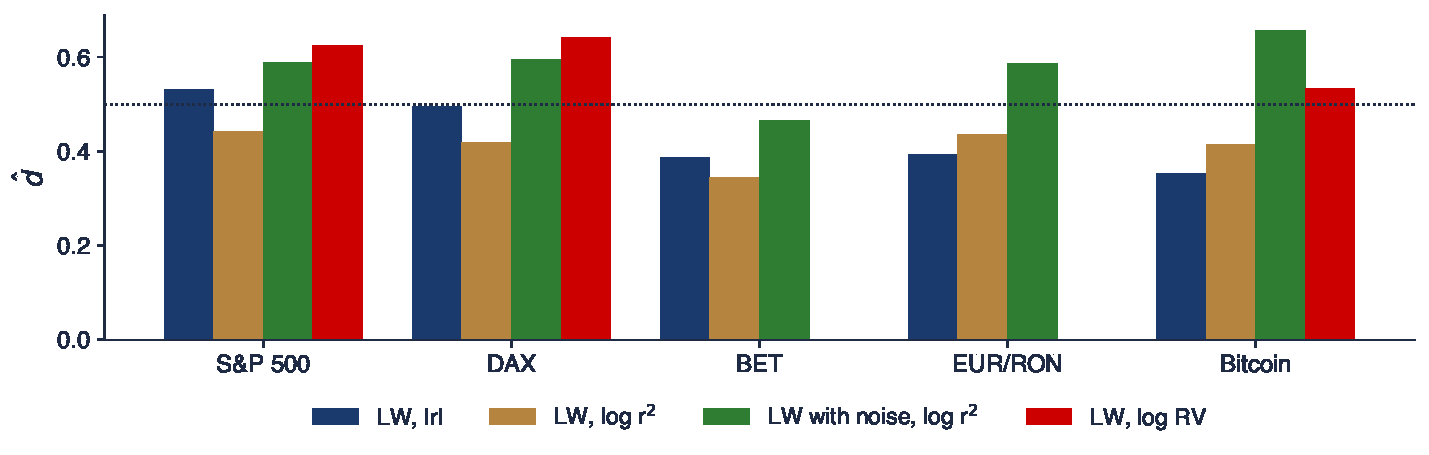
\includegraphics[width=0.97\textwidth,height=0.59\textheight,keepaspectratio]{ats_ch10_assets_d.pdf}
\end{center}
\vspace{-0.25cm}
\begin{itemize}
    \item Local Whittle $\hat d$ with $m = n^{0.65}$ of $|r_t|$ and $\log(r_t^2 + c)$, $c$ = 1\% of the variance; LW with noise on $\log(r_t^2 + c)$ with $m = n^{0.8}$; log RV where realised measures exist (S\&P 500, DAX to 2022; Bitcoin to 2026)
\end{itemize}
\quantlet{ATS\_ch10\_figarch}{\qlurl{ATS_ch10_figarch}}
\end{frame}

\begin{frame}{Interpreting volatility memory across markets}
\itemsize{\small}
\begin{itemize}
    \item S\&P 500: $|r|$ 0.53, $\log r^2$ 0.44, with noise 0.59, log RV 0.62: the noise correction moves $\log r^2$ to the RV level
    \item Bitcoin: $\log r^2$ 0.41, with noise 0.66, log RV 0.53; DAX: 0.42, 0.59, 0.64
    \item Qu test on $|r_t|$ (1\% value 1.56): S\&P 500 0.78, DAX 0.72, Bitcoin 0.79; BET 1.71 and EUR/RON 1.88 reject
    \item For the BET and the leu, part of the apparent memory comes from regime changes (2008, the managed float): model the breaks first (\atschlink{https://danpele.github.io/Advanced-Time-Series/EN/Courses/chapter2_structural_breaks_nonlinear_models.pdf}{Chapter 2})
\end{itemize}
\end{frame}

\begin{frame}{HAR as an approximation of long memory}
\itemsize{\small}
\begin{itemize}
    \item HAR \refCor\ on $y = \log RV$ (\atschlink{https://danpele.github.io/Advanced-Time-Series/EN/Courses/chapter8_advanced_volatility.pdf}{Chapter 8})
    \[ y_{t+1} = \beta_0 + \beta_dy_t + \beta_w\bar y_t^{(5)} + \beta_m\bar y_t^{(22)} + u_{t+1} \]
    \begin{itemize}
        \item $\bar y_t^{(5)}$, $\bar y_t^{(22)}$: averages of $y$ over the last 5 and 22 days; an AR(22) with three free slopes: a step-function approximation of hyperbolically decaying AR weights
    \end{itemize}
    \item Formally short memory: its ACF decays geometrically, but over horizons up to a few months it mimics $k^{2d-1}$
    \begin{itemize}
        \item cascade interpretation: traders with daily, weekly and monthly horizons (heterogeneous market hypothesis)
    \end{itemize}
    \item Estimated by OLS, easy to extend (jumps, semivariances, \atschlink{https://danpele.github.io/Advanced-Time-Series/EN/Courses/chapter8_advanced_volatility.pdf}{Chapter 8}): the benchmark every long-memory or rough model must beat
\end{itemize}
\end{frame}

\begin{frame}{HAR weights and the ACF it implies}
\itemsize{\footnotesize}
\begin{center}
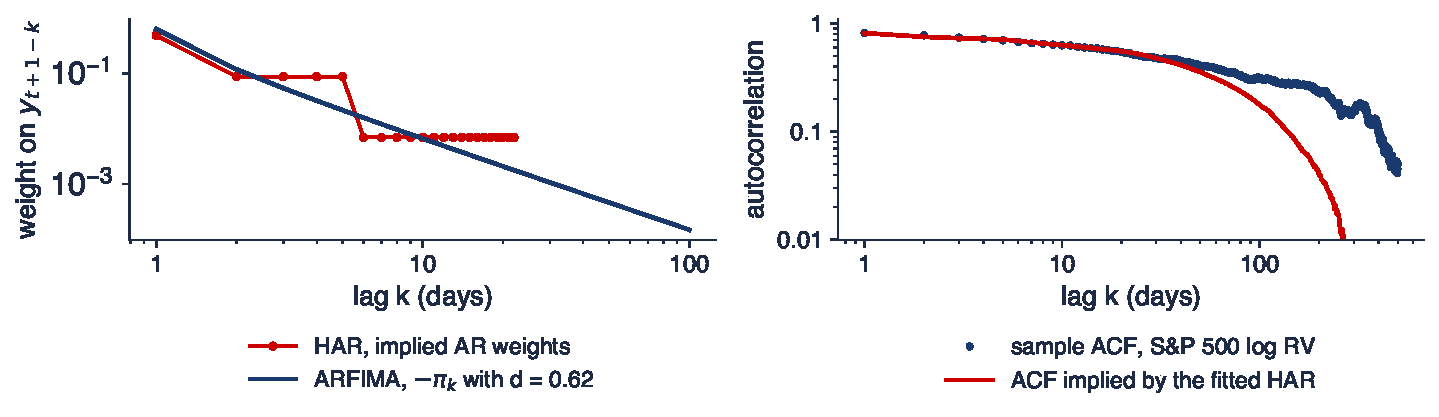
\includegraphics[width=0.97\textwidth,height=0.54\textheight,keepaspectratio]{ats_ch10_har_approx.pdf}
\end{center}
\vspace{-0.25cm}
\begin{itemize}
    \item S\&P 500 log RV; HAR by OLS: $\beta_d = 0.39$, $\beta_w = 0.40$, $\beta_m = 0.15$; left: implied AR weights and ARFIMA $-\pi_k$ with $d = 0.62$; right: ACF of a long simulation of the fitted HAR and the sample ACF
\end{itemize}
\quantlet{ATS\_ch10\_figarch}{\qlurl{ATS_ch10_figarch}}
\end{frame}

\begin{frame}{Interpreting the HAR approximation}
\itemsize{\small}
\begin{itemize}
    \item Sum of HAR weights 0.946: close to a unit root, which is how a short-memory model buys persistence
    \item ACF at lag 100: sample 0.31, HAR 0.179; at lag 250: 0.18 against 0.017
    \item The implied ACF falls below half the sample ACF after lag 112: HAR captures memory up to about half a year
    \item For forecasts up to a month this is enough, which is why HAR is hard to beat (Section 7)
\end{itemize}
\end{frame}

\begin{frame}{Recap: Long memory in volatility}
\itemsize{\small}
\begin{itemize}
    \item FIGARCH has hyperbolic ARCH weights but infinite variance; HYGARCH nests it
    \item $\log r_t^2$ is long memory plus large noise: use the noise-robust LW or realised measures
    \item HAR is a short-memory model that mimics long memory over the horizons that matter for forecasting
\end{itemize}
\end{frame}


%=============================================================================
\section{Rough volatility}
%=============================================================================

\begin{frame}{Fractional Brownian motion (1/2)}
\itemsize{\footnotesize}
\begin{columns}[T]
\begin{column}{0.32\textwidth}
\centering
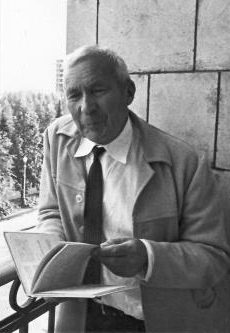
\includegraphics[height=0.25\textheight]{ch10_kolmogorov.jpg}\\[1mm]
\imgcap{A. N. Kolmogorov}
\imgcredit{https://commons.wikimedia.org/wiki/File:Andrej_Nikolajewitsch_Kolmogorov.jpg}{Photo: Konrad Jacobs; CC BY-SA 2.0 de; Wikimedia Commons}\\[1mm]\centering
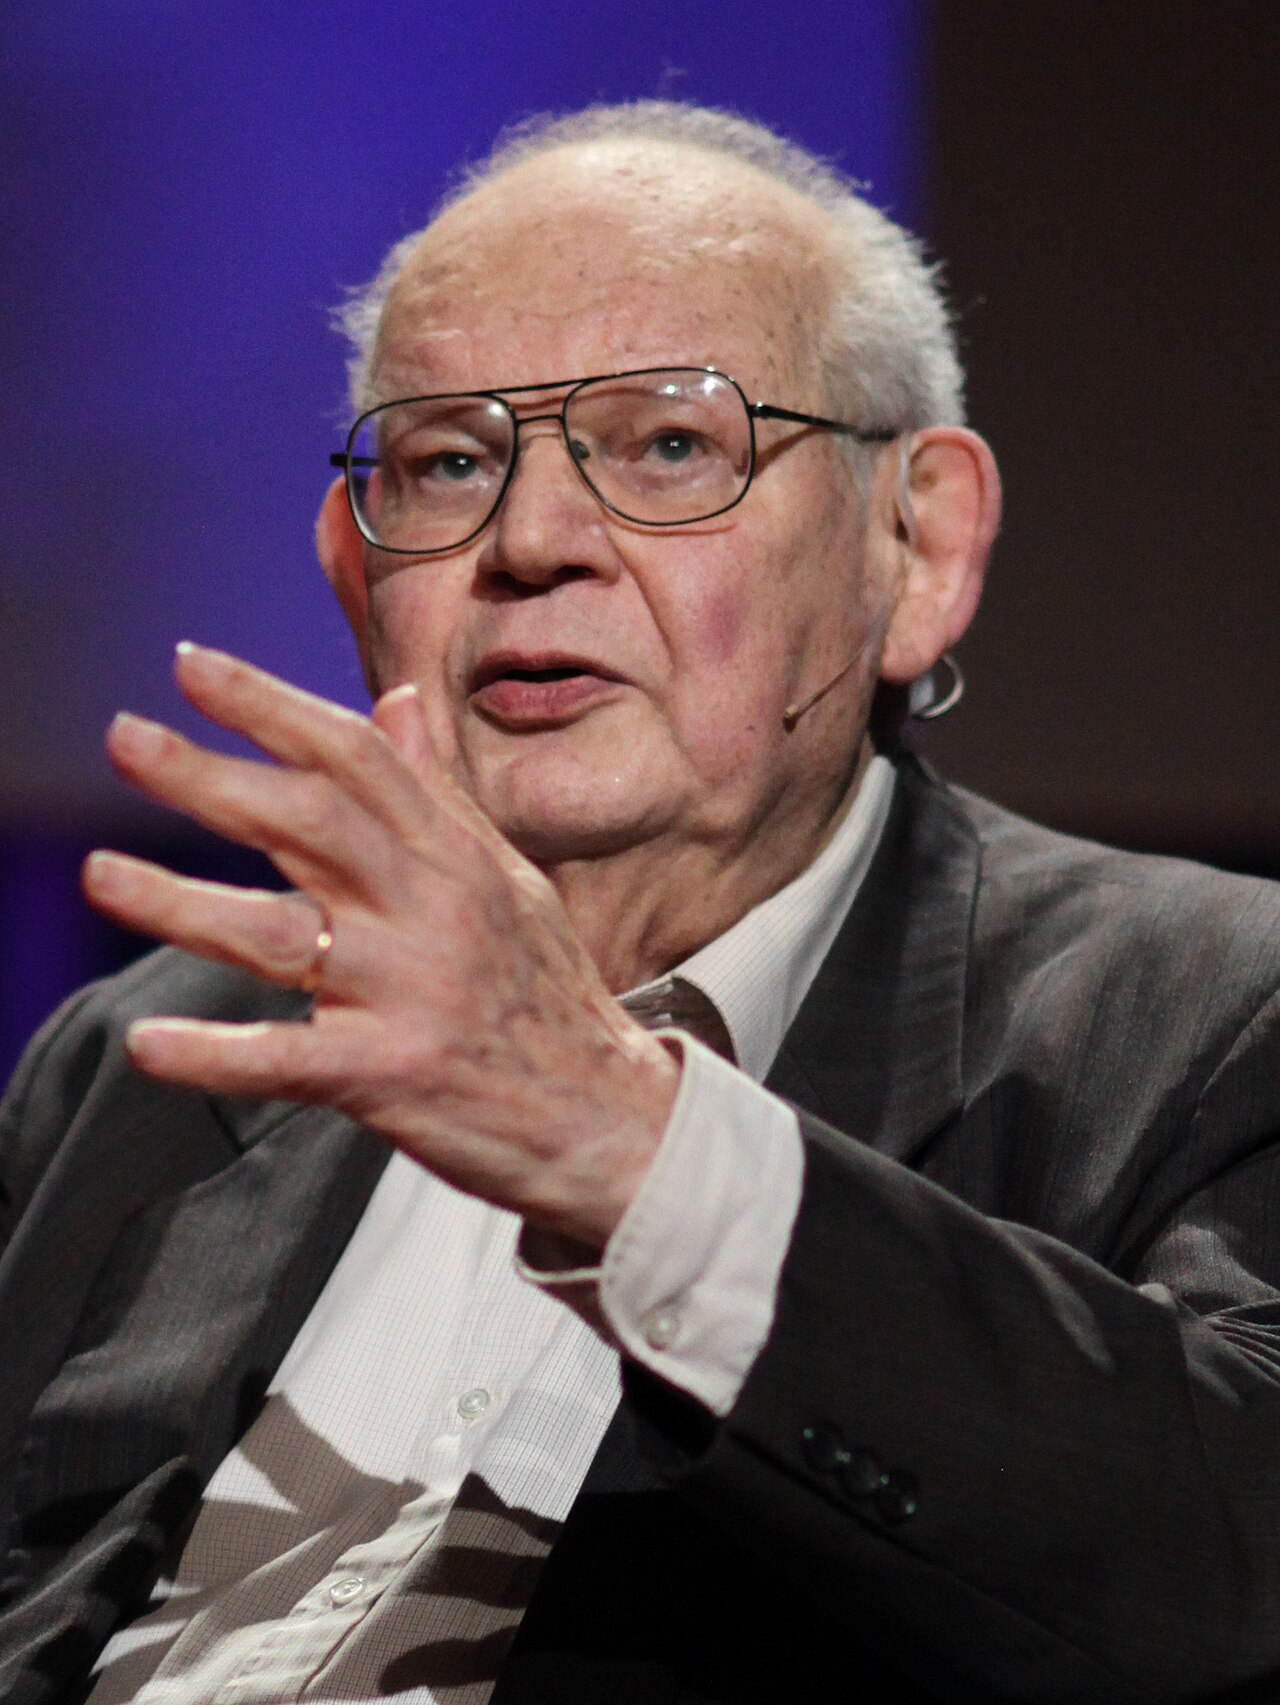
\includegraphics[height=0.15\textheight]{ch10_mandelbrot_2010.jpg}\\[1mm]
\imgcap{B. B. Mandelbrot, TED 2010}
\imgcredit{https://commons.wikimedia.org/wiki/File:Benoit_Mandelbrot,_TED_2010_(3x4_cropped).jpg}{Photo: Steve Jurvetson (2010); CC BY 2.0; Wikimedia Commons}
\end{column}
\begin{column}{0.66\textwidth}
\begin{itemize}
    \item fBm $W^H_t$ \refMVN: a centred Gaussian process with $W^H_0 = 0$ and covariance
    \[ \E W^H_tW^H_s = \frac12\big(t^{2H} + s^{2H} - |t - s|^{2H}\big), \qquad H \in (0, 1) \]
    \begin{itemize}
        \item $H$: the Hurst exponent; $H = 1/2$ gives standard Brownian motion
        \item stationary increments with $\E|W^H_{t+\Delta} - W^H_t|^2 = \Delta^{2H}$
        \item self-similar: $W^H_{ct} \overset{d}{=} c^HW^H_t$ (equal in distribution) for $c > 0$
    \end{itemize}
\end{itemize}
\end{column}
\end{columns}
\end{frame}

\begin{frame}{Fractional Brownian motion (2/2)}
\itemsize{\small}
\begin{itemize}
    \item Paths are Hölder continuous of every order $< H$
    \begin{itemize}
        \item Hölder order: how fast $|W^H_{t+\Delta} - W^H_t|$ can shrink with $\Delta$; $H < 1/2$: rougher (more irregular), $H > 1/2$: smoother than Brownian motion
    \end{itemize}
    \item The increments, fractional Gaussian noise (fGn), have autocorrelations
    \[ \rho(k) = \frac12\big(|k + 1|^{2H} - 2|k|^{2H} + |k - 1|^{2H}\big) \sim H(2H - 1)k^{2H-2} \]
    \begin{itemize}
        \item long memory for $H > 1/2$ ($d = H - 1/2$); negative correlation for $H < 1/2$
    \end{itemize}
\end{itemize}
\end{frame}

\begin{frame}{Fractional Brownian paths}
\itemsize{\footnotesize}
\begin{center}
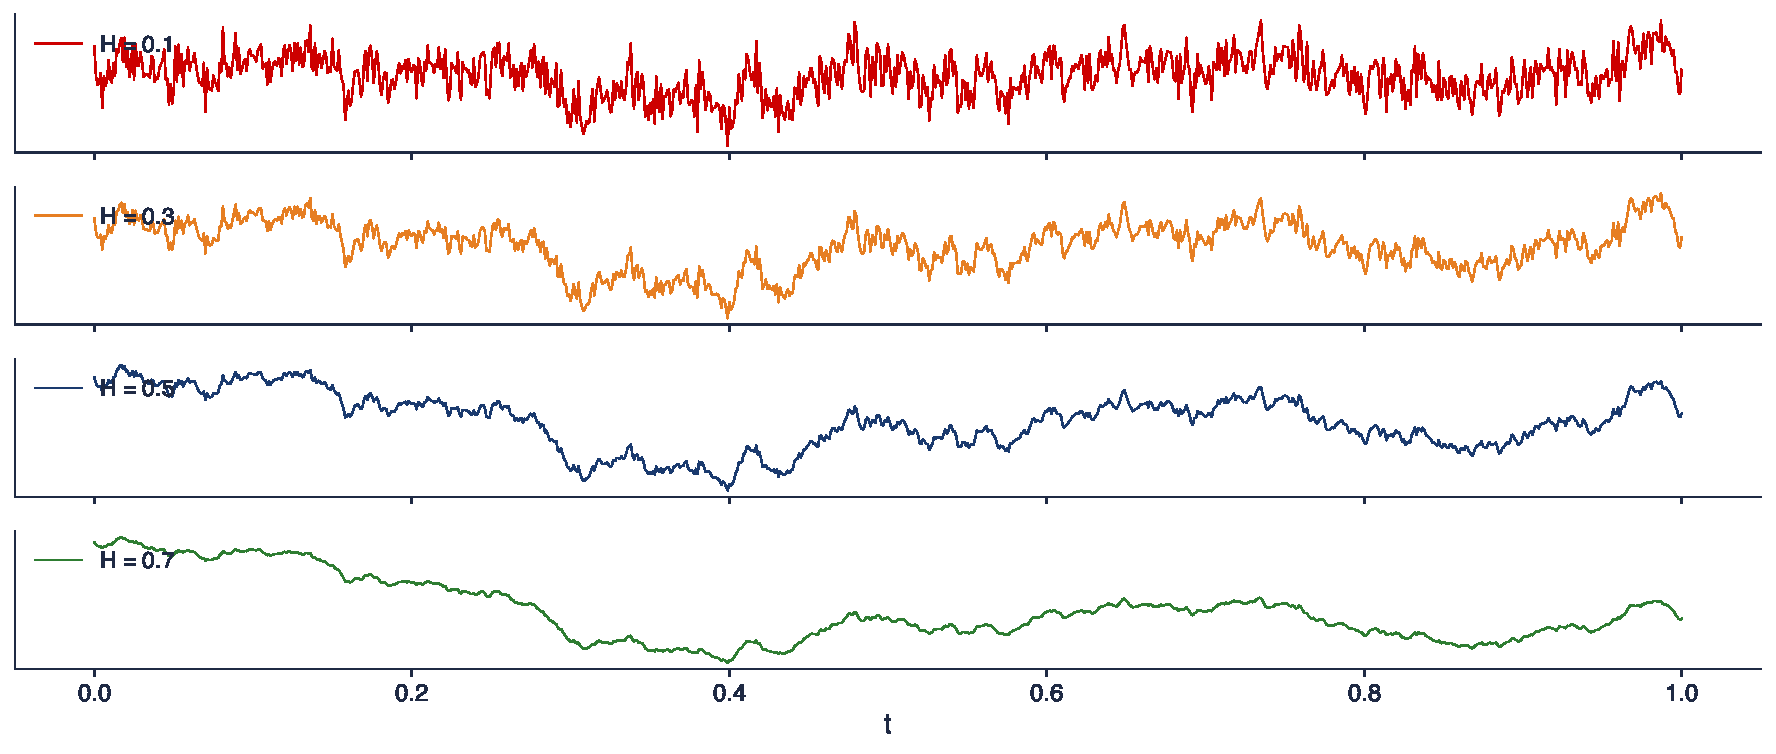
\includegraphics[width=0.97\textwidth,height=0.65\textheight,keepaspectratio]{ats_ch10_fbm_paths.pdf}
\end{center}
\vspace{-0.25cm}
\begin{itemize}
    \item One path each on 1000 steps, exact simulation by circulant embedding; $H = 0.5$ is Brownian motion
\end{itemize}
\quantlet{ATS\_ch10\_simulation}{\qlurl{ATS_ch10_simulation}}
\end{frame}

\begin{frame}{Interpreting the paths}
\itemsize{\small}
\begin{itemize}
    \item Lag-one correlation of the increments: \ensuremath{-}0.426 for $H = 0.1$, \ensuremath{-}0.242 for $H = 0.3$, 0 for $H = 0.5$, 0.320 for $H = 0.7$
    \item $H = 0.1$: every rise is likely to be followed by a fall, so the path is jagged at all scales but wanders little
    \item $H = 0.7$: trends persist; this is the fBm reading of the Hurst effect
    \item Roughness is a statement about small scales, persistence about large ones: keep the two apart
\end{itemize}
\end{frame}

\begin{frame}{Simulating fBm: Cholesky, circulant embedding}
\itemsize{\small}
\begin{itemize}
    \item Cholesky: $\Gamma = LL'$, $X = LZ$; exact but $O(n^3)$ time and $O(n^2)$ memory
    \begin{itemize}
        \item $\Gamma$: the $n \times n$ covariance matrix of the path; $L$: its lower-triangular Cholesky factor; $Z$: a vector of i.i.d. $N(0, 1)$
    \end{itemize}
    \item Davies--Harte \refDH, \refDN: embed the Toeplitz $\Gamma$ of fGn in a circulant matrix of order $M = 2(n - 1)$ with first row $c = (\gamma_0, \dots, \gamma_{n-1}, \gamma_{n-2}, \dots, \gamma_1)$
    \begin{itemize}
        \item $\gamma_k$: autocovariances of fGn; a circulant matrix is diagonalised by the discrete Fourier transform: eigenvalues $\Lambda = \mathrm{FFT}(c)$
        \item if $\Lambda \ge 0$: $Y = \mathrm{FFT}\big(\sqrt{\Lambda/M}\,(Z_1 + iZ_2)\big)$, $Z_1, Z_2$ independent standard Gaussian vectors; $\mathrm{Re}\,Y$ and $\mathrm{Im}\,Y$ are two independent exact paths
    \end{itemize}
    \item $O(n\log n)$; for fGn $\Lambda \ge 0$ for every $H$ (Seminar 10, A7); fBm = cumulated fGn
    \item The same algorithm simulates ARFIMA$(0,d,0)$ exactly (used in every Monte Carlo of this chapter)
\end{itemize}
\end{frame}

\begin{frame}{The hybrid scheme for Volterra processes}
\itemsize{\footnotesize}
\begin{itemize}
    \item Rough volatility models use Volterra processes, not stationary-increment fBm \refBFG
    \[ X_t = \int_0^tg(t - s)\,dW_s, \qquad g(x) = x^{H-1/2} \ \ \text{(Riemann--Liouville)} \]
    \begin{itemize}
        \item $g$: the kernel, singular at 0 when $H < 1/2$; $W$: Brownian motion; circulant embedding does not apply (non-stationary, possibly non-Gaussian when driven by a correlated price)
    \end{itemize}
    \item Hybrid scheme \refBLPa: integrate the kernel exactly on the last step, use a Riemann sum at optimal points further away
    \[ X_i \approx \int_{t_{i-1}}^{t_i}(t_i - s)^{H-1/2}dW_s + \sum_{k\ge2}\Big(\frac{b_k}{n}\Big)^{H-1/2}\Delta W_{i-k+1} \]
    \[ b_k = \Big(\frac{k^{H+1/2} - (k - 1)^{H+1/2}}{H + 1/2}\Big)^{1/(H-1/2)} \]
    \begin{itemize}
        \item $n$: steps per unit of time; $\Delta W_i$: Brownian increments; $b_k$: the optimal evaluation point in cell $k$; the first term and $\Delta W_i$ are jointly Gaussian and simulated exactly
    \end{itemize}
    \item The sum is a convolution: $O(n\log n)$ by FFT; the scheme extends to Brownian semistationary processes
\end{itemize}
\end{frame}

\begin{frame}{Riemann sum against the hybrid scheme}
\itemsize{\footnotesize}
\begin{center}
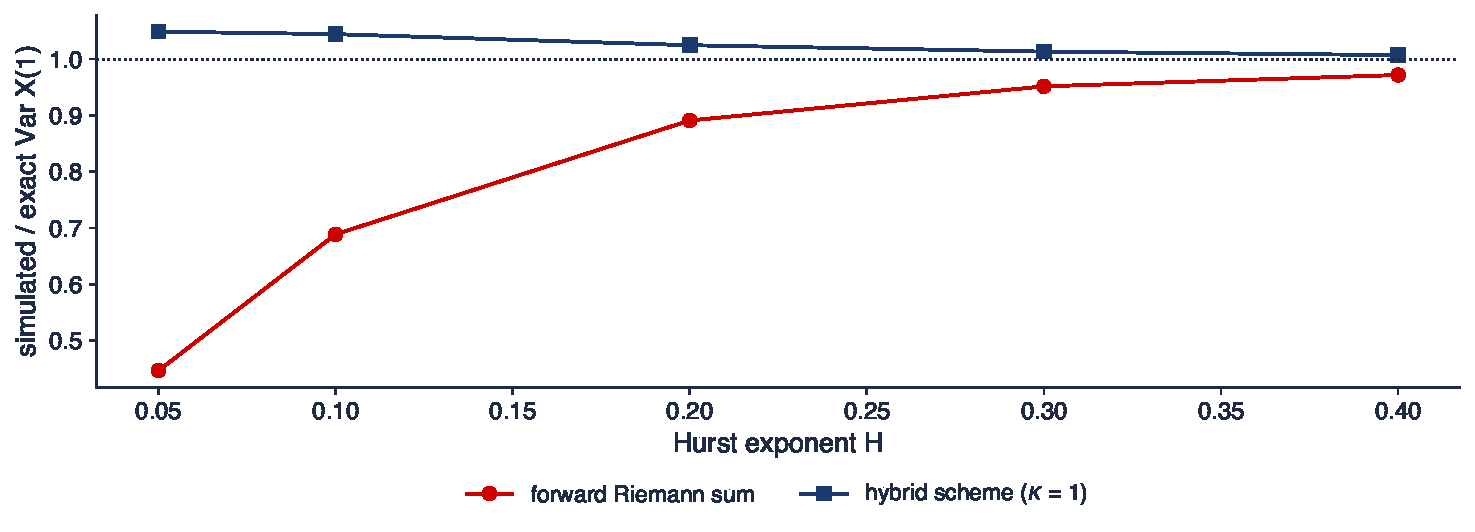
\includegraphics[width=0.97\textwidth,height=0.67\textheight,keepaspectratio]{ats_ch10_hybrid.pdf}
\end{center}
\vspace{-0.25cm}
\begin{itemize}
    \item $\Var X(1)$ of the Riemann--Liouville process, exact value $1/(2H)$; $n = 250$ steps, 4\,000 paths
\end{itemize}
\quantlet{ATS\_ch10\_simulation}{\qlurl{ATS_ch10_simulation}}
\end{frame}

\begin{frame}{Interpreting the simulation schemes}
\itemsize{\small}
\begin{itemize}
    \item Forward Riemann sum: 0.45 of the true variance at $H = 0.05$ and 0.69 at $H = 0.1$: it misses the mass of the kernel near the singularity
    \item Hybrid scheme: 1.05 and 1.04, within Monte Carlo error of 1
    \item The error of the naive scheme grows exactly where rough volatility lives ($H \approx 0.1$): option prices from it would be biased
\end{itemize}
\end{frame}

\begin{frame}{The evidence: scaling of log volatility (1/2)}
\itemsize{\small}
\begin{itemize}
    \item \refGJR, Section 2: from daily $\sigma_t = \sqrt{RV_t}$ (Oxford-Man library), the empirical moments of the increments of $\log\sigma$
    \[ m(q, \Delta) = \frac1N\sum_t|\log\sigma_{t+\Delta} - \log\sigma_t|^q \]
    \begin{itemize}
        \item $\Delta$: lag in days; $q > 0$: order of the moment; $N$: number of pairs; $m(2, \Delta)$ is the variogram
    \end{itemize}
    \item If $\log\sigma$ has fBm-like increments, the moments scale as a power of $\Delta$ (monofractal scaling)
    \[ m(q, \Delta) = K_q\nu^q\Delta^{\zeta_q}, \qquad \zeta_q = qH \]
    \begin{itemize}
        \item $\nu$: volatility of volatility; $K_q = \E|Z|^q$, $Z \sim N(0, 1)$; $\zeta_q$: scaling exponent, linear in $q$ with slope $H$
        \item derivation and deviations from this scaling: \atsapplink{atsapp2}{atssrc2}{Appendix}  % applink: scaling of fBm moments
    \end{itemize}
\end{itemize}
\end{frame}

\begin{frame}{The evidence: scaling of log volatility (2/2)}
\itemsize{\small}
\begin{itemize}
    \item Procedure: OLS of $\log m(q, \Delta)$ on $\log\Delta$ for each $q$ gives $\zeta_q$; regress $\zeta_q$ on $q$ through the origin to get $H$
    \begin{itemize}
        \item we use $q \in \{0.5, 1, 1.5, 2, 3\}$ and $\Delta = 1, \dots, 50$ days
    \end{itemize}
    \item Their finding: linear $\zeta_q$ and $H$ of order 0.1 for all indices; the increments of log volatility are close to Gaussian
    \item This contradicts every Markovian SV model (Heston, log-OU), whose log volatility has $H = 1/2$ at short lags
\end{itemize}
\end{frame}

\begin{frame}{Replicating the scaling on the S\&P 500}
\itemsize{\footnotesize}
\begin{center}
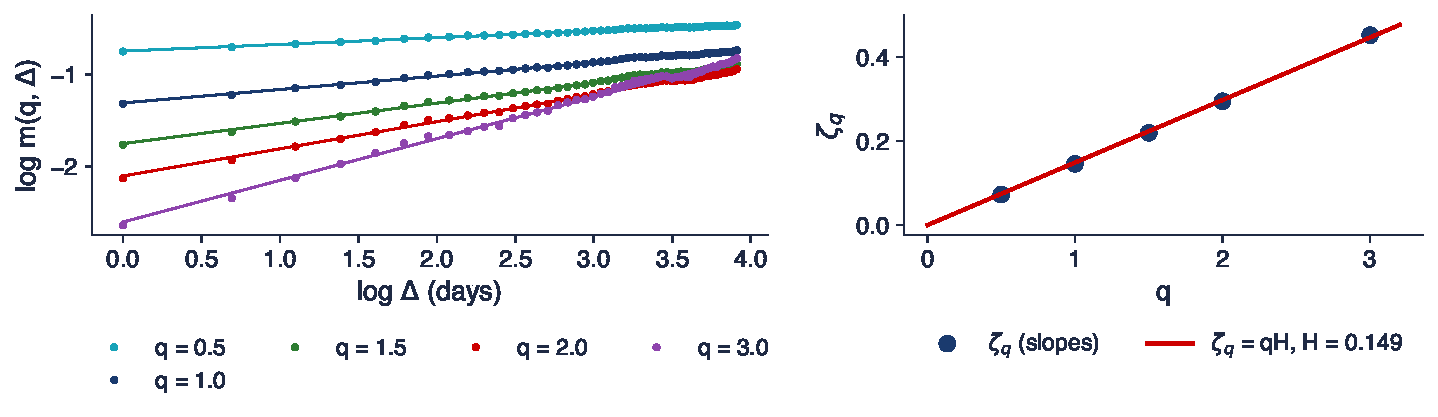
\includegraphics[width=0.97\textwidth,height=0.54\textheight,keepaspectratio]{ats_ch10_gjr.pdf}
\end{center}
\vspace{-0.25cm}
\begin{itemize}
    \item Oxford-Man 5-minute RV of the S\&P 500, January 2000 -- February 2022; left: $\log m(q, \Delta)$ and OLS lines; right: $\zeta_q$ and the line $qH$
\end{itemize}
\quantlet{ATS\_ch10\_rough}{\qlurl{ATS_ch10_rough}}
\end{frame}

\begin{frame}{Interpreting the scaling}
\itemsize{\small}
\begin{itemize}
    \item $\zeta_q$ = 0.073, 0.146, 0.220, 0.295, 0.452 for $q$ = 0.5, 1, 1.5, 2, 3: linear in $q$, $\hat H = 0.149$
    \item Vol-of-vol $\hat\nu = 0.35$ from $m(2, \Delta) = \nu^2\Delta^{2H}$; subsamples: 0.140 (2000--2010), 0.155 (2011--2022)
    \item The paper's result replicates: roughly $H \approx 0.1$ to 0.15, stable over time
\end{itemize}
\end{frame}

\begin{frame}{The RFSV model}
\itemsize{\small}
\begin{itemize}
    \item \refGJR: rough fractional stochastic volatility (RFSV), log volatility a fractional Ornstein--Uhlenbeck (OU) process
    \[ \sigma_t = \exp(X_t), \qquad dX_t = \nu\,dW^H_t - \alpha(X_t - m)\,dt, \qquad H < 1/2 \]
    \begin{itemize}
        \item $\nu$: volatility of volatility; $m$: long-run mean of $X$; $\alpha > 0$: speed of mean reversion, very small
        \item for $\alpha T \ll 1$ ($T$: sample span) the increments behave like those of $\nu W^H$; stationarity only shows at horizons of order $1/\alpha$
    \end{itemize}
    \item The link with long memory: over observable horizons $\log\sigma$ is close to a non-stationary fBm with $H \approx 0.1$, whose ARFIMA reading is $d = H + 1/2$ (0.65 for the S\&P 500, close to the local Whittle $\hat d$ of log RV)
    \begin{itemize}
        \item GJR show that local Whittle and similar estimators applied to RFSV simulations return the ``long-memory'' values found in the literature
    \end{itemize}
    \item Pricing: rough Bergomi \refBFG\ and rough Heston \refER
    \begin{itemize}
        \item both fit the term structure of the implied-volatility skew, $\propto \tau^{H-1/2}$ ($\tau$: option maturity), with few parameters
        \item option-based estimates also give small $H$ \refLMPR
        \item the pricing side belongs to MFM; here we test the time-series claim
    \end{itemize}
\end{itemize}
\end{frame}

\begin{frame}{Roughness across markets and proxies}
\itemsize{\footnotesize}
\begin{center}
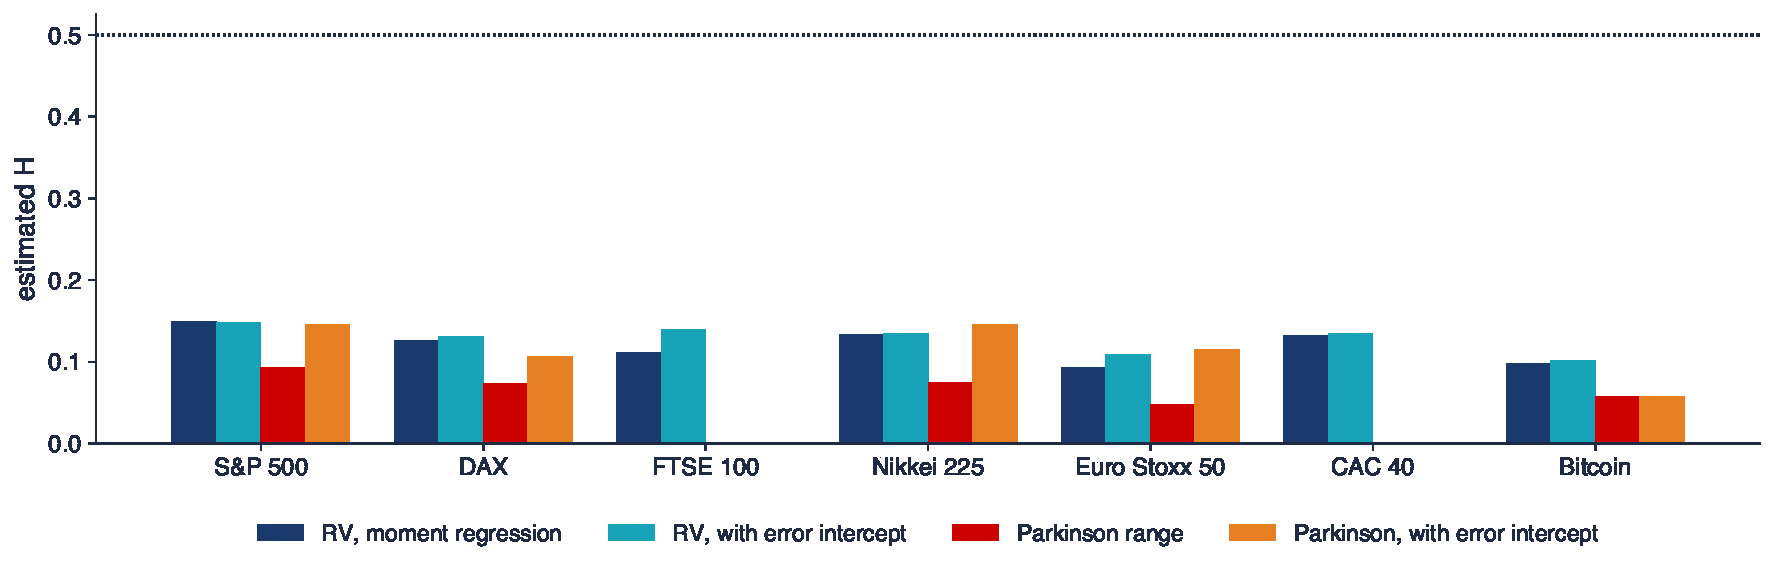
\includegraphics[width=0.97\textwidth,height=0.59\textheight,keepaspectratio]{ats_ch10_gjr_assets.pdf}
\end{center}
\vspace{-0.25cm}
\begin{itemize}
    \item $H$ from 5-minute RV (Oxford-Man; Bitcoin: Binance) by the moment regression and with a measurement-error intercept; Parkinson range of EODHD daily highs and lows over the same days, where available
\end{itemize}
\quantlet{ATS\_ch10\_rough}{\qlurl{ATS_ch10_rough}}
\end{frame}

\begin{frame}{Interpreting roughness across markets}
\itemsize{\small}
\begin{itemize}
    \item RV: $H$ from 0.093 to 0.149 for six indices and Bitcoin (S\&P 500 0.149, DAX 0.127, Euro Stoxx 50 0.093, Bitcoin 0.098)
    \item The error intercept changes little (S\&P 500 0.148); only for the FTSE 100 does it absorb 31\% of $m(2, 1)$
    \item Parkinson range, a much noisier proxy: S\&P 500 0.09, DAX 0.07; with the intercept 0.15 and 0.11 (noise share 52\% and 42\%)
    \item Measurement error pushes $H$ down; the correction brings the range back near the RV estimate, but not above it
\end{itemize}
\end{frame}

\begin{frame}{Critiques: is roughness an artefact?}
\itemsize{\small}
\begin{itemize}
    \item RV is an estimate of integrated variance: $\log RV_t = \log\int_{t-1}^t\sigma_s^2ds + \epsilon_t$
    \begin{itemize}
        \item two opposite biases: daily integration smooths (pushes $\hat H$ up), the error $\epsilon_t$ adds a nugget to $m(2, \Delta)$ (pushes $\hat H$ down)
    \end{itemize}
    \item \refFTW: a Whittle-type estimator consistent under high-frequency asymptotics with measurement error; volatility remains rough, $H$ even below 0.1
    \begin{itemize}
        \item \refBCPV: GMM on the moments of integrated variance with noise; also small $H$
    \end{itemize}
    \item \refCD: the roughness estimators applied to RV can report small $H$ even for smooth (Markovian) volatility: a finite-sample artefact of the proxy
    \begin{itemize}
        \item the answer depends on the size of the error relative to the daily variation of log volatility: simulate it
    \end{itemize}
\end{itemize}
\end{frame}

\begin{frame}{Measurement error and the estimate of $H$}
\itemsize{\footnotesize}
\begin{center}
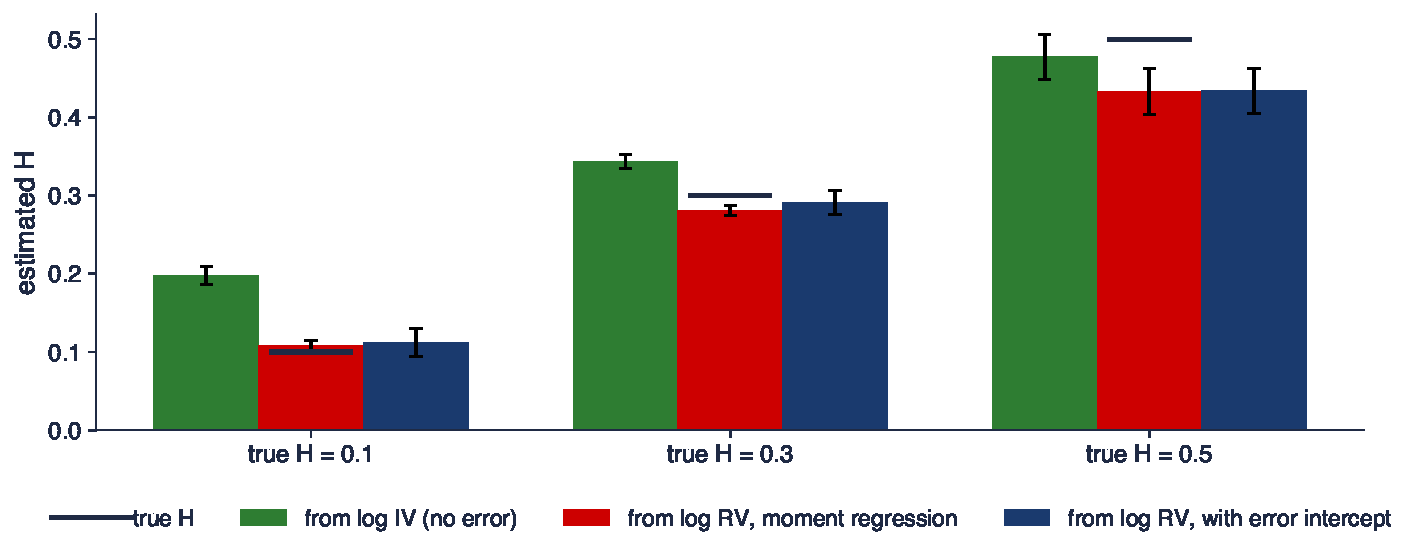
\includegraphics[width=0.97\textwidth,height=0.65\textheight,keepaspectratio]{ats_ch10_noise_sim.pdf}
\end{center}
\vspace{-0.25cm}
\begin{itemize}
    \item Log volatility a fractional OU on 78 intraday steps a day, 2\,500 days, 8 replications; daily IV (no error) and RV from the 78 squared returns; GJR estimator
\end{itemize}
\quantlet{ATS\_ch10\_rough}{\qlurl{ATS_ch10_rough}}
\end{frame}

\begin{frame}{Interpreting the simulation}
\itemsize{\small}
\begin{itemize}
    \item True $H = 0.1$: from IV 0.20, from RV 0.11, RV with intercept 0.11: the integration bias and the error bias almost cancel
    \item True $H = 0.5$: IV 0.48, RV 0.43, with intercept 0.43; true $H = 0.3$: 0.34, 0.28, 0.29
    \item With 5-minute RV the error is too small to turn $H = 0.5$ into the 0.1--0.15 seen in the data
    \item A noisier proxy (Parkinson, squared returns) or a different volatility model could; the conclusion is conditional on this design
\end{itemize}
\end{frame}

\begin{frame}{Roughness and persistence}
\itemsize{\small}
\begin{itemize}
    \item In fBm one parameter fixes both: small $H$ means rough paths and (for increments) antipersistence
    \begin{itemize}
        \item Cauchy and gamma-kernel models separate the fractal dimension (short scales) from the Hurst effect (long scales) \refGS
    \end{itemize}
    \item \refBLPb: Brownian semistationary model $X_t = \int_{-\infty}^tg(t - s)\,dW_s$, $g(x) \approx x^\alpha$ near 0 (roughness, $H = \alpha + 1/2$), $g(x) \approx x^{-\beta}$ at infinity (memory)
    \begin{itemize}
        \item their finding: log volatility is both rough ($\alpha < 0$) and persistent ($\beta < 1$); the two are estimated separately
    \end{itemize}
    \item Empirical check: slope of the variogram at short lags against the decay of the ACF at long lags
\end{itemize}
\end{frame}

\begin{frame}{Short scales and long scales}
\itemsize{\footnotesize}
\begin{center}
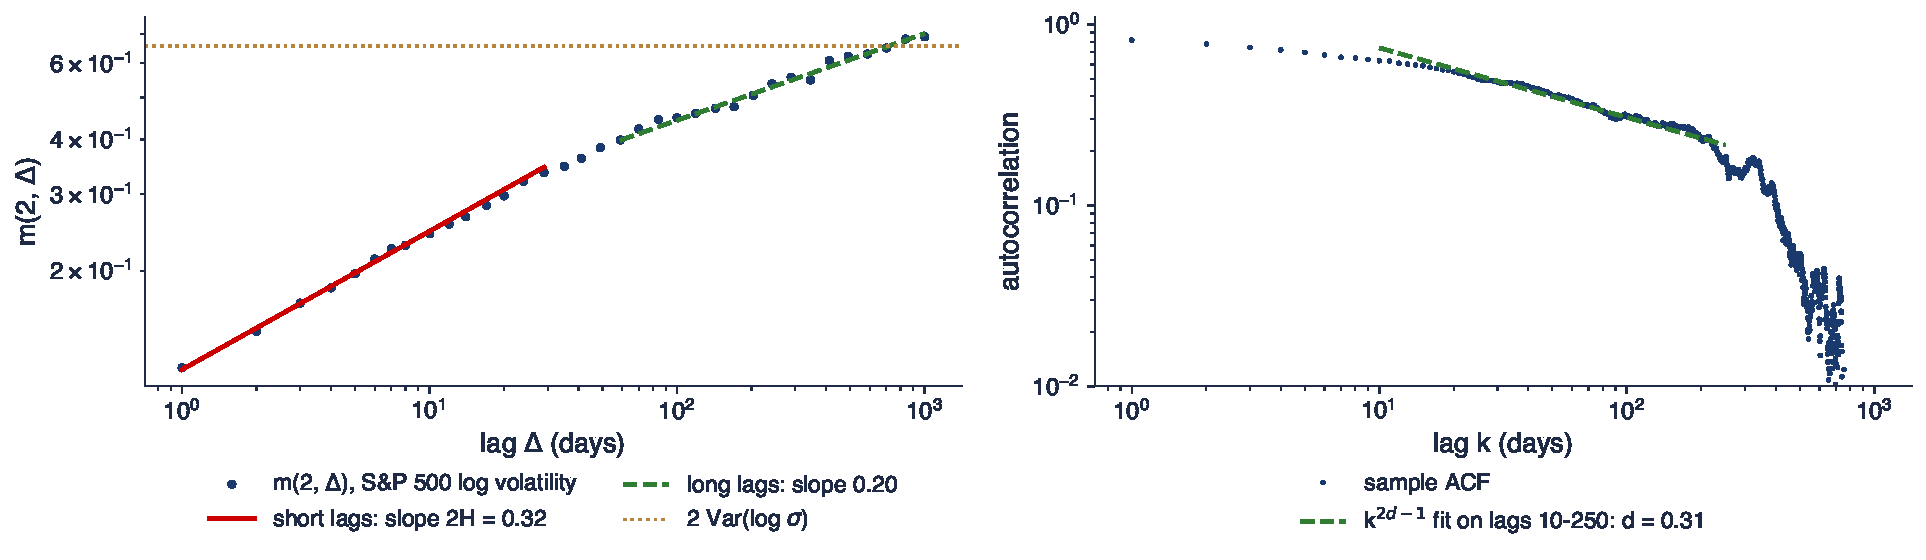
\includegraphics[width=0.97\textwidth,height=0.54\textheight,keepaspectratio]{ats_ch10_decouple.pdf}
\end{center}
\vspace{-0.25cm}
\begin{itemize}
    \item S\&P 500 log volatility, lags 1--1000 days; left: variogram $m(2, \Delta)$ with slopes on lags 1--10 and 100--1000; right: sample ACF with a $k^{2d-1}$ fit on lags 10--250
\end{itemize}
\quantlet{ATS\_ch10\_rough}{\qlurl{ATS_ch10_rough}}
\end{frame}

\begin{frame}{Interpreting the two scales}
\itemsize{\small}
\begin{itemize}
    \item Short lags: slope $2H = 0.32$, $H = 0.16$; long lags: slope 0.20, still rising at 1000 days, above $2\Var(\log\sigma)$
    \item Read as a non-stationary fractional process, the long-lag slope $2d - 1$ gives $d = 0.60$; local Whittle with $m = 74$ gives 0.56
    \item The ACF fit gives only $d = 0.31$: the sample ACF is biased down when $d$ is near or above 1/2
    \item Rough at short scales, highly persistent at long scales: both claims hold for the same series
\end{itemize}
\end{frame}

\begin{frame}{Recap: Rough volatility}
\itemsize{\small}
\begin{itemize}
    \item fBm with $H < 1/2$: rough paths; simulate it exactly by circulant embedding, Volterra versions by the hybrid scheme
    \item The scaling of log RV gives $H \approx 0.1$--0.15 on every market we tried, stable over time
    \item Measurement error and daily integration bias $\hat H$ in opposite directions; roughness and persistence are separate properties
\end{itemize}
\end{frame}


%=============================================================================
\section{Forecasting realised variance: rough, long memory, HAR}
%=============================================================================

\begin{frame}{The RFSV predictor (1/2)}
\itemsize{\small}
\begin{itemize}
    \item For fBm (Nuzman--Poor), with $\alpha \approx 0$, \refGJR, Section 5: the forecast of log variance is a weighted average of its past
    \[ \E[\log\sigma^2_{t+h} \mid \mathcal F_t] = \frac{\cos(H\pi)}{\pi}\,h^{H+1/2}\int_{-\infty}^t\frac{\log\sigma_s^2}{(t - s + h)(t - s)^{H+1/2}}\,ds \]
    \begin{itemize}
        \item $h$: forecast horizon; $\mathcal F_t$: the past of volatility up to $t$; the kernel integrates to one, with more weight on the recent past for small $H$
        \item discretised on days: $w_k = \int_k^{k+1}du/((u + h)u^{H+1/2})$, truncated at 500 days and normalised
    \end{itemize}
\end{itemize}
\end{frame}

\begin{frame}{The RFSV predictor (2/2): the variance forecast}
\itemsize{\small}
\begin{itemize}
    \item From log variance to variance: a lognormal correction
    \[ \E[\sigma^2_{t+h} \mid \mathcal F_t] = \exp\big(\E[\log\sigma^2_{t+h} \mid \mathcal F_t] + 2c\nu^2h^{2H}\big) \]
    \[ c = \frac{\Gamma(3/2 - H)}{\Gamma(H + 1/2)\Gamma(2 - 2H)} \]
    \begin{itemize}
        \item $2c\nu^2h^{2H}$: half the conditional variance of $\log\sigma^2_{t+h}$, which grows with the horizon; with the S\&P 500 values $c = 0.707$
    \end{itemize}
    \item Two parameters ($H$, $\nu$), both from the variogram: no likelihood, no optimisation
\end{itemize}
\end{frame}

\begin{frame}{How far back the forecasts look}
\itemsize{\footnotesize}
\begin{center}
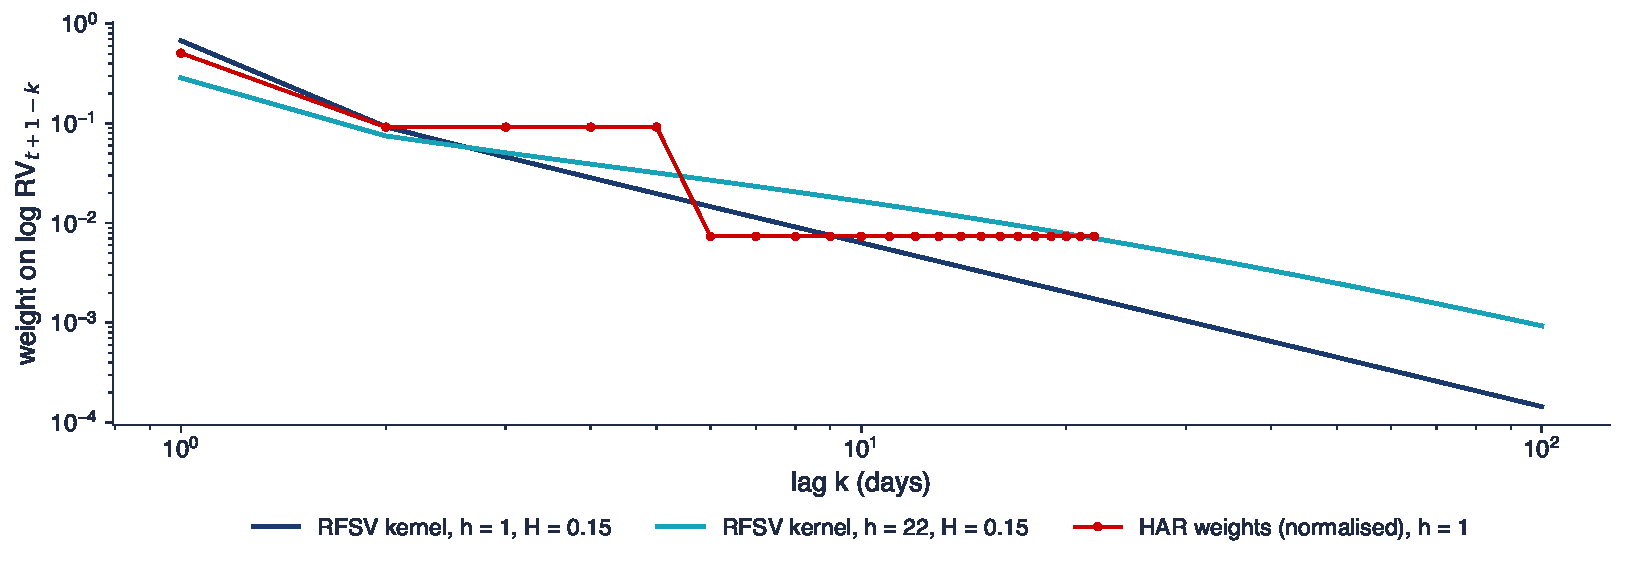
\includegraphics[width=0.97\textwidth,height=0.64\textheight,keepaspectratio]{ats_ch10_rfsv_kernel.pdf}
\end{center}
\vspace{-0.25cm}
\begin{itemize}
    \item RFSV kernel with $H = 0.15$ (S\&P 500) for $h = 1$ and $h = 22$ days, against the normalised HAR weights for $h = 1$
\end{itemize}
\quantlet{ATS\_ch10\_forecast}{\qlurl{ATS_ch10_forecast}}
\end{frame}

\begin{frame}{Interpreting the kernels}
\itemsize{\small}
\begin{itemize}
    \item $h = 1$: RFSV puts 68\% on the last day, 86\% on the last week, 95\% on the last month; HAR: 51\% and 87\%
    \item $h = 22$: only 29\% on the last day, 71\% on the last month, 90\% within 100 days: longer horizons look further back
    \item The kernel adapts its memory to the horizon automatically; HAR needs a separate regression for each horizon
    \item RFSV has no mean reversion: in long calm periods it does not pull forecasts towards a long-run level
\end{itemize}
\end{frame}

\begin{frame}{An honest out-of-sample comparison}
\itemsize{\small}
\begin{itemize}
    \item Design fixed in advance: rolling window of 1000 days, parameters re-estimated every 20 days with data up to $t$ only; target $RV_{t+h}$, $h \in \{1, 5, 22\}$
    \begin{itemize}
        \item HAR: direct regression of $\log RV_{t+h}$; ARFIMA$(0,d,0)$: local Whittle $d$ (capped at 0.49), AR($\infty$) iterated; RFSV: $H$, $\nu$ from the window
    \end{itemize}
    \item Loss: QLIKE $L = RV/F - \log(RV/F) - 1$, robust to the noise in the RV proxy \refPat; also MSE of logs
    \begin{itemize}
        \item level forecasts from log forecasts need the lognormal correction: $\exp(\hat\mu + \hat s^2/2)$ for HAR and ARFIMA, $2c\nu^2h^{2H}$ for RFSV
    \end{itemize}
    \item Inference: DM with Newey--West variance (\atschlink{https://danpele.github.io/Advanced-Time-Series/EN/Courses/chapter1_forecast_evaluation.pdf}{Chapter 1}) \refDM; the loss differences are themselves persistent, so the $p$-values are optimistic
\end{itemize}
\end{frame}

\begin{frame}{RFSV and ARFIMA against HAR}
\itemsize{\footnotesize}
\begin{center}
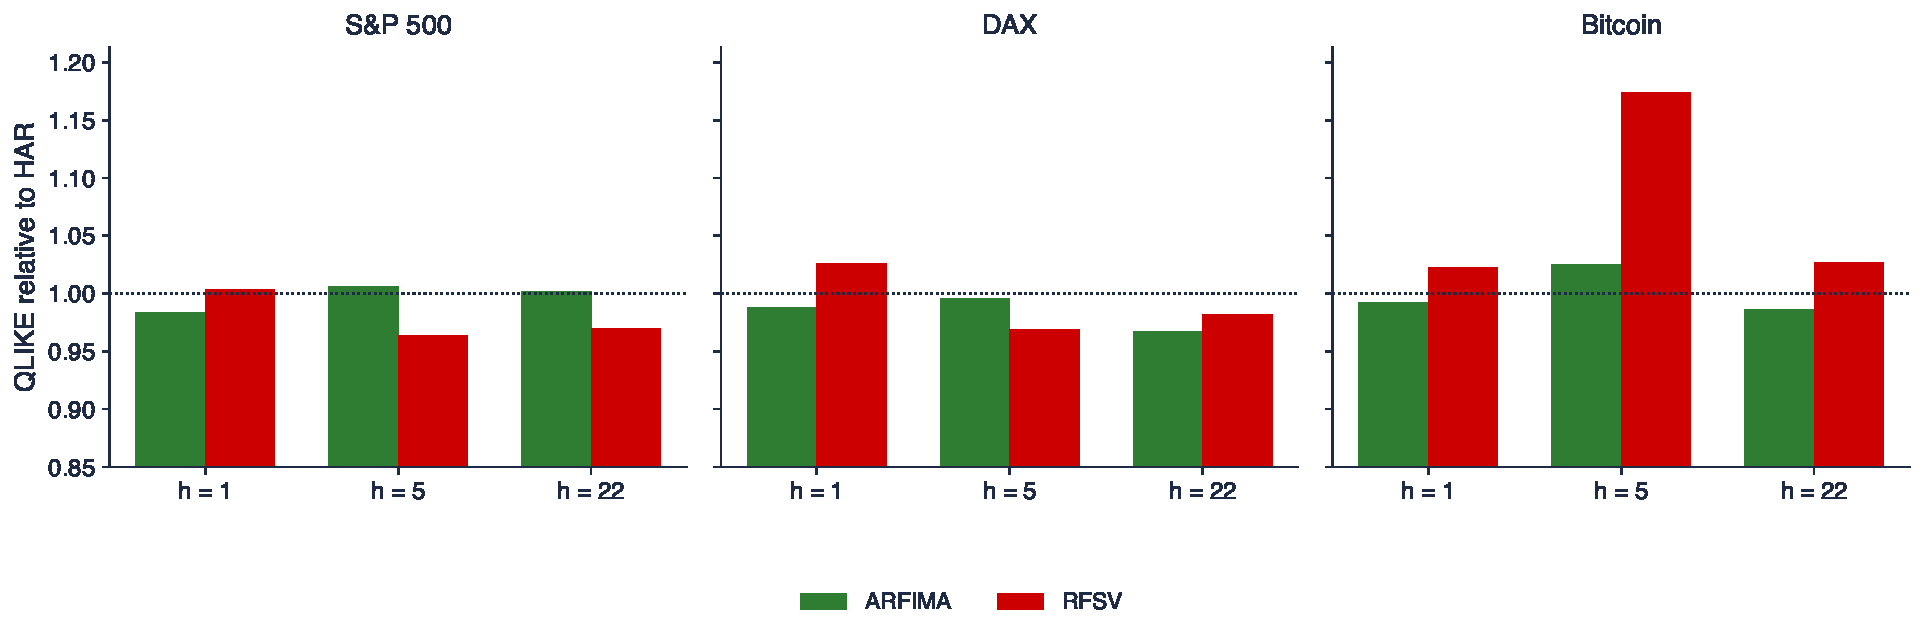
\includegraphics[width=0.97\textwidth,height=0.56\textheight,keepaspectratio]{ats_ch10_forecast.pdf}
\end{center}
\vspace{-0.25cm}
\begin{itemize}
    \item Average QLIKE relative to HAR (below 1: better than HAR); a star marks a DM $p$-value below 5\%; S\&P 500 6 January 2004 -- 24 January 2022 ($T = 4\,531$), DAX ($T = 4\,593$), Bitcoin 10 October 2020 -- 27 August 2026 ($T = 2\,144$)
\end{itemize}
\quantlet{ATS\_ch10\_forecast}{\qlurl{ATS_ch10_forecast}}
\end{frame}

\begin{frame}{Interpreting the forecast comparison}
\itemsize{\footnotesize}
\begin{center}
\scriptsize
\begin{tabular}{lcccccc}
\toprule
\textbf{QLIKE / HAR} & \multicolumn{2}{c}{S\&P 500} & \multicolumn{2}{c}{DAX} & \multicolumn{2}{c}{Bitcoin} \\ & ARFIMA & RFSV & ARFIMA & RFSV & ARFIMA & RFSV \\
\midrule
$h = 1$ & 0.984 & 1.003 & 0.988 & 1.026 & 0.992 & 1.022 \\
$h = 5$ & 1.006 & 0.964 & 0.996 & 0.969 & 1.025 & 1.174 \\
$h = 22$ & 1.002 & 0.969 & 0.968 & 0.982 & 0.986 & 1.027 \\
\bottomrule
\end{tabular}
\end{center}
\begin{itemize}
    \item S\&P 500 and DAX: RFSV is 1.8\% to 3.6\% better than HAR at 5 and 22 days but worse at 1 day; DM at 5 days: \ensuremath{-}1.78 ($p$ 0.07) and \ensuremath{-}1.62 ($p$ 0.11)
    \item Bitcoin: RFSV is worse at every horizon (1.174 at 5 days); rolling $\hat H$ ranges from 0.04 to 0.15, median 0.08
    \item ARFIMA is within 3.2\% of HAR everywhere; of the 18 QLIKE comparisons, none is significant at 5\%
    \item Roughness is a robust stylised fact; its forecasting gain over HAR is small and horizon-dependent, as in \refGJR\ and \refWXY
\end{itemize}
\end{frame}

\begin{frame}{Recap: Forecasting}
\itemsize{\small}
\begin{itemize}
    \item RFSV forecasts with a horizon-dependent power kernel and a lognormal correction, from two variogram parameters
    \item Out of sample, RFSV, ARFIMA and HAR are close; RFSV gains a few percent at weekly and monthly horizons for equity indices
    \item Pre-register the design, use QLIKE, and treat DM $p$-values with care under persistent loss differences
\end{itemize}
\end{frame}


%=============================================================================
\section{AI for scientific discovery}
%=============================================================================

\begin{frame}{An open question}
\itemsize{\small}
\begin{itemize}
    \item Is the roughness of volatility a property of the volatility process, or of the way we measure it?
    \begin{itemize}
        \item formal: $H_0$: $H \ge 0.3$ for integrated variance; tested with estimators that are consistent under measurement error, on pre-registered assets, measures and samples
        \item falsified if the corrected estimates stay below 0.2 across sampling frequencies and markets
    \end{itemize}
    \item Why it matters: rough models change option pricing and hedging; if roughness is an artefact, Markovian models suffice
    \begin{itemize}
        \item literature to start from: \refGJR, \refFTW, \refBCPV, \refCD, \refBLPb
    \end{itemize}
\end{itemize}
\end{frame}

\begin{frame}{The discovery loop with an AI assistant}
\itemsize{\footnotesize}
\begin{itemize}
    \item An AI assistant (an LLM such as Claude, ChatGPT, Gemini or Copilot) speeds up each step; Semantic Scholar and Elicit help with the literature
    \begin{itemize}
        \item \textbf{literature}: \aiprompt{List peer-reviewed papers since 2018 that estimate the Hurst exponent of volatility with methods robust to measurement error; give DOIs.} Then check every DOI on Crossref
        \item \textbf{hypothesis}: \aiprompt{Which data-generating processes with H = 0.5 would make the moment estimator on 5-minute RV return H near 0.1?}
        \item \textbf{code and replication}: ask for the variogram regression, then reproduce first the S\&P 500 value (0.149 here) and the simulation table
        \item \textbf{critique}: \aiprompt{Act as a hostile referee: list how lag choice, overnight returns, jumps and microstructure noise could bias H.}
    \end{itemize}
    \item Report: what was asked, what was kept, what was rejected (AI\_USE.md, AI\_ERRORS.md)
\end{itemize}
\end{frame}

\begin{frame}{What the human checks}
\itemsize{\small}
\begin{itemize}
    \item Every reference exists and says what is claimed (DOI resolves, title matches, the result is in the paper)
    \item The scale is stated: $H$ of fBm, $d$ of ARFIMA, $H = d + 1/2$ for stationary series; log volatility or log variance
    \item Bandwidths, lags and trimming are reported, with estimates across a range, not one convenient choice
    \item Breaks and level shifts are tested (Qu) before long memory is claimed
    \item Forecast comparisons are out of sample, pre-registered, with QLIKE and DM
\end{itemize}
\end{frame}

\begin{frame}{Mini-case: how robust is ``$H$ of order 0.1''?}
\itemsize{\footnotesize}
\begin{center}
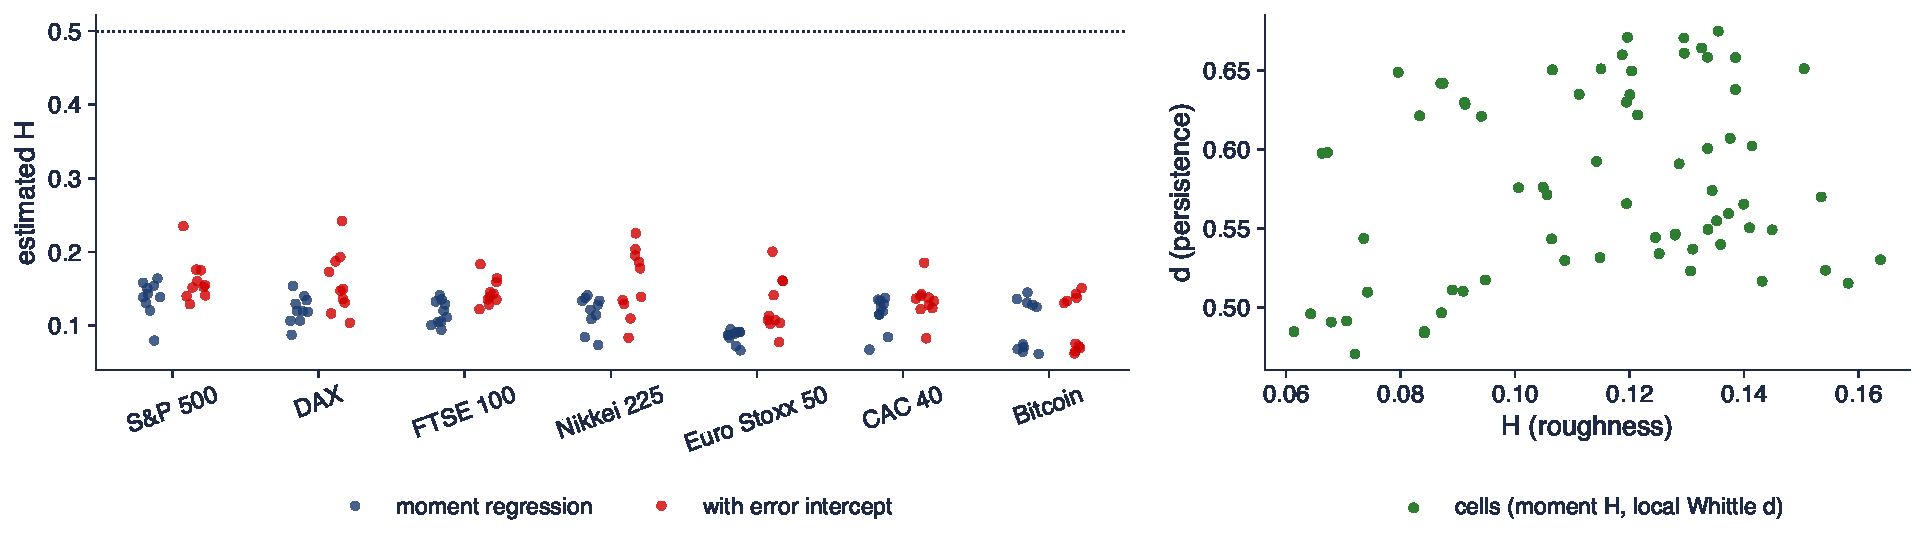
\includegraphics[width=0.97\textwidth,height=0.52\textheight,keepaspectratio]{ats_ch10_ai_case.pdf}
\end{center}
\vspace{-0.25cm}
\begin{itemize}
    \item 70 cells: seven assets $\times$ five realised measures $\times$ two halves of the sample; two estimators each (140 estimates); right: $H$ against the local Whittle $d$ of the same cell
    \item $H$ from 0.06 to 0.24, median 0.13 (moments 0.12, with intercept 0.14); 96\% below 0.2; $d$ from 0.47 to 0.68; correlation of $H$ and $d$ 0.24: an AI summary that calls volatility ``short memory because $H < 1/2$'' is wrong
\end{itemize}
\quantlet{ATS\_ch10\_rough}{\qlurl{ATS_ch10_rough}}
\end{frame}

\begin{frame}{Project idea}
\itemsize{\small}
\begin{itemize}
    \item \textbf{Roughness and persistence of volatility in Central and Eastern European markets}: replicate first, then extend
    \begin{itemize}
        \item replicate: \refGJR, Section 2 on the Oxford-Man S\&P 500 ($H = 0.149$ here) and the forecasting comparison of their Section 5
        \item extend: intraday data for the BET, WIG20 and EUR/RON; estimators robust to noise (FTW, GMM); Qu tests; a BSS model with separate roughness and memory
        \item pre-register: assets, measures, lags, bandwidths, the forecast design and the loss
    \end{itemize}
    \item Deliverables follow the course rules: repository, report, AI\_USE.md, AI\_ERRORS.md, oral defence
\end{itemize}
\end{frame}


%=============================================================================
\section{Wrap-up}
%=============================================================================

\begin{frame}{Key takeaways}
\itemsize{\small}
\begin{itemize}
    \item Long memory is a pole at frequency zero; estimate it with local Whittle or exact local Whittle and report $\hat d(m)$
    \item Level shifts mimic long memory: test with Qu (2011) and look at the bandwidth signature
    \item Volatility is persistent over months (FIGARCH, LMSV, HAR) and rough over days ($H \approx 0.1$)
    \item Proxies matter: noise lowers $\hat d$ and $\hat H$; corrections exist and should be reported
    \item In forecasting, HAR remains a tough benchmark; rough models gain little and only at some horizons
\end{itemize}
\end{frame}

\begin{frame}{Self-assessment}
\itemsize{\small}
\begin{columns}[T]
\begin{column}{0.58\textwidth}
\begin{block}{Questions}
\begin{itemize}
    \item Why is the asymptotic variance of local Whittle $1/(4m)$ and that of GPH $\pi^2/(24m)$?
    \item Why does local Whittle fail for $d > 1$, and how does exact local Whittle fix it?
    \item Which spectral shape does a random level shift produce?
    \item Why is FIGARCH not covariance stationary?
    \item How can a series be rough and long-memory at the same time?
\end{itemize}
\end{block}
\end{column}
\begin{column}{0.38\textwidth}
\begin{block}{Next: \atschlink{https://danpele.github.io/Advanced-Time-Series/EN/Courses/chapter11_spectral_wavelet_analysis.pdf}{Chapter 11}}
\begin{itemize}
    \item Spectral and wavelet analysis
    \item multitaper, coherence, wavelets: the frequency tools behind this chapter
\end{itemize}
\end{block}
\end{column}
\end{columns}
\end{frame}


%=============================================================================
\section{Appendix}
%=============================================================================

\begin{frame}{Appendix: the variance of local Whittle}
\hypertarget{atsapp1}{}\atsappback{atssrc1}{Back}
\itemsize{\small}
\begin{itemize}
    \item Expand $R'(\hat d) = 0$ around $d$: $\sqrt m(\hat d - d) = -\sqrt m\,R'(d)/R''(\bar d)$
    \item $\sqrt m\,R'(d) = \dfrac{2}{\sqrt m}\sum_j\nu_j(\xi_j - 1) + o_p(1)$, $\xi_j = \lambda_j^{2d}I(\lambda_j)/G$; with $\Var\xi_j \to 1$ and $\frac1m\sum\nu_j^2 \to 1$: $\to N(0, 4)$
    \item $R''(d) = \dfrac4m\sum_j\nu_j^2\xi_j/\bar\xi - \big(\dfrac2m\sum_j\nu_j\xi_j/\bar\xi\big)^2 \to_p 4$
    \item Hence $\sqrt m(\hat d - d) \to N(0, 4/16) = N(0, 1/4)$; for GPH the same weights multiply $\log\xi_j$ with variance $\pi^2/6$: $N(0, \pi^2/24)$
\end{itemize}
\end{frame}

\begin{frame}{Appendix: scaling of fBm moments}
\hypertarget{atsapp2}{}\atsappback{atssrc2}{Back}
\itemsize{\small}
\begin{itemize}
    \item $W^H_{t+\Delta} - W^H_t \sim N(0, \Delta^{2H})$, so $\E|W^H_{t+\Delta} - W^H_t|^q = \Delta^{qH}\E|Z|^q$, $\E|Z|^q = 2^{q/2}\Gamma\big(\tfrac{q+1}{2}\big)/\sqrt\pi$
    \item With $\log\sigma_t = \nu W^H_t$: $\log m(q, \Delta) = q\log\nu + \log\E|Z|^q + qH\log\Delta$: slope $\zeta_q = qH$
    \item Departures: concave $\zeta_q$ signals multifractality or heavy tails; an intercept in $m(2, \Delta) = \nu^2\Delta^{2H} + 2s^2$ signals i.i.d.\ measurement error of variance $s^2$
    \item fGn spectrum near zero: $f(\lambda) \propto |\lambda|^{1-2H}$, i.e.\ the increments are ARFIMA-like with $d = H - 1/2$
\end{itemize}
\end{frame}


%=============================================================================
\section{References}
%=============================================================================

\begin{frame}{References (1/4)}
\itemsize{\tiny}
\begin{itemize}
    \item Andersen, T. G., Bollerslev, T., Diebold, F. X., \& Labys, P. (2003). Modeling and forecasting realized volatility. \textit{Econometrica}, 71(2), 579--625. \href{https://doi.org/10.1111/1468-0262.00418}{doi:10.1111/1468-0262.00418}
    \item Andrews, D. W. K., \& Sun, Y. (2004). Adaptive local polynomial Whittle estimation of long-range dependence. \textit{Econometrica}, 72(2), 569--614. \href{https://doi.org/10.1111/j.1468-0262.2004.00501.x}{doi:10.1111/j.1468-0262.2004.00501.x}
    \item Baillie, R. T., Bollerslev, T., \& Mikkelsen, H. O. (1996). Fractionally integrated generalized autoregressive conditional heteroskedasticity. \textit{Journal of Econometrics}, 74(1), 3--30. \href{https://doi.org/10.1016/S0304-4076(95)01749-6}{doi:10.1016/S0304-4076(95)01749-6}
    \item Baillie, R. T., Chung, C.-F., \& Tieslau, M. A. (1996). Analysing inflation by the fractionally integrated ARFIMA--GARCH model. \textit{Journal of Applied Econometrics}, 11(1), 23--40. \href{https://doi.org/10.1002/(SICI)1099-1255(199601)11:1\%3C23::AID-JAE374\%3E3.0.CO;2-M}{doi:10.1002/(SICI)1099-1255(199601)11:1\textless{}23::AID-JAE374\textgreater{}3.0.CO;2-M}
    \item Bandi, F. M., \& Perron, B. (2006). Long memory and the relation between implied and realized volatility. \textit{Journal of Financial Econometrics}, 4(4), 636--670. \href{https://doi.org/10.1093/jjfinec/nbl003}{doi:10.1093/jjfinec/nbl003}
    \item Bayer, C., Friz, P., \& Gatheral, J. (2016). Pricing under rough volatility. \textit{Quantitative Finance}, 16(6), 887--904. \href{https://doi.org/10.1080/14697688.2015.1099717}{doi:10.1080/14697688.2015.1099717}
    \item Bennedsen, M., Lunde, A., \& Pakkanen, M. S. (2022). Decoupling the short- and long-term behavior of stochastic volatility. \textit{Journal of Financial Econometrics}, 20(5), 961--1006. \href{https://doi.org/10.1093/jjfinec/nbaa049}{doi:10.1093/jjfinec/nbaa049}
    \item Bennedsen, M., Lunde, A., \& Pakkanen, M. S. (2017). Hybrid scheme for Brownian semistationary processes. \textit{Finance and Stochastics}, 21(4), 931--965. \href{https://doi.org/10.1007/s00780-017-0335-5}{doi:10.1007/s00780-017-0335-5}
    \item Beran, J., Feng, Y., Ghosh, S., \& Kulik, R. (2013). \textit{Long-Memory Processes: Probabilistic Properties and Statistical Methods}. Springer. \href{https://doi.org/10.1007/978-3-642-35512-7}{doi:10.1007/978-3-642-35512-7}
    \item Bolko, A. E., Christensen, K., Pakkanen, M. S., \& Veliyev, B. (2023). A GMM approach to estimate the roughness of stochastic volatility. \textit{Journal of Econometrics}, 235(2), 745--778. \href{https://doi.org/10.1016/j.jeconom.2022.06.009}{doi:10.1016/j.jeconom.2022.06.009}
    \item Breidt, F. J., Crato, N., \& de Lima, P. (1998). The detection and estimation of long memory in stochastic volatility. \textit{Journal of Econometrics}, 83(1--2), 325--348. \href{https://doi.org/10.1016/S0304-4076(97)00072-9}{doi:10.1016/S0304-4076(97)00072-9}
    \item Christensen, B. J., \& Nielsen, M. Ø. (2006). Asymptotic normality of narrow-band least squares in the stationary fractional cointegration model and volatility forecasting. \textit{Journal of Econometrics}, 133(1), 343--371. \href{https://doi.org/10.1016/j.jeconom.2005.03.018}{doi:10.1016/j.jeconom.2005.03.018}
    \item Comte, F., \& Renault, E. (1998). Long memory in continuous-time stochastic volatility models. \textit{Mathematical Finance}, 8(4), 291--323. \href{https://doi.org/10.1111/1467-9965.00057}{doi:10.1111/1467-9965.00057}
    \item Cont, R., \& Das, P. (2024). Rough volatility: Fact or artefact? \textit{Sankhya B}, 86(1), 191--223. \href{https://doi.org/10.1007/s13571-024-00322-2}{doi:10.1007/s13571-024-00322-2}
\end{itemize}
\end{frame}

\begin{frame}{References (2/4)}
\itemsize{\tiny}
\begin{itemize}
    \item Corsi, F. (2009). A simple approximate long-memory model of realized volatility. \textit{Journal of Financial Econometrics}, 7(2), 174--196. \href{https://doi.org/10.1093/jjfinec/nbp001}{doi:10.1093/jjfinec/nbp001}
    \item Davidson, J. (2004). Moment and memory properties of linear conditional heteroscedasticity models, and a new model. \textit{Journal of Business \& Economic Statistics}, 22(1), 16--29. \href{https://doi.org/10.1198/073500103288619359}{doi:10.1198/073500103288619359}
    \item Davies, R. B., \& Harte, D. S. (1987). Tests for Hurst effect. \textit{Biometrika}, 74(1), 95--101. \href{https://doi.org/10.1093/biomet/74.1.95}{doi:10.1093/biomet/74.1.95}
    \item Diebold, F. X., \& Inoue, A. (2001). Long memory and regime switching. \textit{Journal of Econometrics}, 105(1), 131--159. \href{https://doi.org/10.1016/S0304-4076(01)00073-2}{doi:10.1016/S0304-4076(01)00073-2}
    \item Diebold, F. X., \& Mariano, R. S. (1995). Comparing predictive accuracy. \textit{Journal of Business \& Economic Statistics}, 13(3), 253--263. \href{https://doi.org/10.1080/07350015.1995.10524599}{doi:10.1080/07350015.1995.10524599}
    \item Dietrich, C. R., \& Newsam, G. N. (1997). Fast and exact simulation of stationary Gaussian processes through circulant embedding of the covariance matrix. \textit{SIAM Journal on Scientific Computing}, 18(4), 1088--1107. \href{https://doi.org/10.1137/S1064827592240555}{doi:10.1137/S1064827592240555}
    \item El Euch, O., \& Rosenbaum, M. (2019). The characteristic function of rough Heston models. \textit{Mathematical Finance}, 29(1), 3--38. \href{https://doi.org/10.1111/mafi.12173}{doi:10.1111/mafi.12173}
    \item Fox, R., \& Taqqu, M. S. (1986). Large-sample properties of parameter estimates for strongly dependent stationary Gaussian time series. \textit{The Annals of Statistics}, 14(2), 517--532. \href{https://doi.org/10.1214/aos/1176349936}{doi:10.1214/aos/1176349936}
    \item Fukasawa, M., Takabatake, T., \& Westphal, R. (2022). Consistent estimation for fractional stochastic volatility model under high-frequency asymptotics. \textit{Mathematical Finance}, 32(4), 1086--1132. \href{https://doi.org/10.1111/mafi.12354}{doi:10.1111/mafi.12354}
    \item Gatheral, J., Jaisson, T., \& Rosenbaum, M. (2018). Volatility is rough. \textit{Quantitative Finance}, 18(6), 933--949. \href{https://doi.org/10.1080/14697688.2017.1393551}{doi:10.1080/14697688.2017.1393551}
    \item Geweke, J., \& Porter-Hudak, S. (1983). The estimation and application of long memory time series models. \textit{Journal of Time Series Analysis}, 4(4), 221--238. \href{https://doi.org/10.1111/j.1467-9892.1983.tb00371.x}{doi:10.1111/j.1467-9892.1983.tb00371.x}
    \item Gneiting, T., \& Schlather, M. (2004). Stochastic models that separate fractal dimension and the Hurst effect. \textit{SIAM Review}, 46(2), 269--282. \href{https://doi.org/10.1137/S0036144501394387}{doi:10.1137/S0036144501394387}
    \item Granger, C. W. J., \& Hyung, N. (2004). Occasional structural breaks and long memory with an application to the S\&P 500 absolute stock returns. \textit{Journal of Empirical Finance}, 11(3), 399--421. \href{https://doi.org/10.1016/j.jempfin.2003.03.001}{doi:10.1016/j.jempfin.2003.03.001}
    \item Granger, C. W. J., \& Joyeux, R. (1980). An introduction to long-memory time series models and fractional differencing. \textit{Journal of Time Series Analysis}, 1(1), 15--29. \href{https://doi.org/10.1111/j.1467-9892.1980.tb00297.x}{doi:10.1111/j.1467-9892.1980.tb00297.x}
\end{itemize}
\end{frame}

\begin{frame}{References (3/4)}
\itemsize{\tiny}
\begin{itemize}
    \item Granger, C. W. J. (1980). Long memory relationships and the aggregation of dynamic models. \textit{Journal of Econometrics}, 14(2), 227--238. \href{https://doi.org/10.1016/0304-4076(80)90092-5}{doi:10.1016/0304-4076(80)90092-5}
    \item Hassler, U., \& Wolters, J. (1995). Long memory in inflation rates: International evidence. \textit{Journal of Business \& Economic Statistics}, 13(1), 37--45. \href{https://doi.org/10.1080/07350015.1995.10524577}{doi:10.1080/07350015.1995.10524577}
    \item Heber, G., Lunde, A., Shephard, N., \& Sheppard, K. K. (2009). Oxford-Man Institute\'s realized library, version 0.3. Oxford-Man Institute, University of Oxford. \href{https://web.archive.org/web/20220301022212/https://realized.oxford-man.ox.ac.uk/}{web.archive.org}
    \item Henry, M., \& Robinson, P. M. (1996). Bandwidth choice in Gaussian semiparametric estimation of long range dependence. In \textit{Athens Conference on Applied Probability and Time Series Analysis}, Lecture Notes in Statistics 115, 220--232. Springer. \href{https://doi.org/10.1007/978-1-4612-2412-9_16}{doi:10.1007/978-1-4612-2412-9\_16}
    \item Hosking, J. R. M. (1981). Fractional differencing. \textit{Biometrika}, 68(1), 165--176. \href{https://doi.org/10.1093/biomet/68.1.165}{doi:10.1093/biomet/68.1.165}
    \item Hurst, H. E. (1951). Long-term storage capacity of reservoirs. \textit{Transactions of the American Society of Civil Engineers}, 116(1), 770--799. \href{https://doi.org/10.1061/TACEAT.0006518}{doi:10.1061/TACEAT.0006518}
    \item Hurvich, C. M., Deo, R., \& Brodsky, J. (1998). The mean squared error of Geweke and Porter-Hudak\'s estimator of the memory parameter of a long-memory time series. \textit{Journal of Time Series Analysis}, 19(1), 19--46. \href{https://doi.org/10.1111/1467-9892.00075}{doi:10.1111/1467-9892.00075}
    \item Hurvich, C. M., Moulines, E., \& Soulier, P. (2005). Estimating long memory in volatility. \textit{Econometrica}, 73(4), 1283--1328. \href{https://doi.org/10.1111/j.1468-0262.2005.00616.x}{doi:10.1111/j.1468-0262.2005.00616.x}
    \item Johansen, S., \& Nielsen, M. Ø. (2012). Likelihood inference for a fractionally cointegrated vector autoregressive model. \textit{Econometrica}, 80(6), 2667--2732. \href{https://doi.org/10.3982/ECTA9299}{doi:10.3982/ECTA9299}
    \item Livieri, G., Mouti, S., Pallavicini, A., \& Rosenbaum, M. (2018). Rough volatility: Evidence from option prices. \textit{IISE Transactions}, 50(9), 767--776. \href{https://doi.org/10.1080/24725854.2018.1444297}{doi:10.1080/24725854.2018.1444297}
    \item Lu, Y. K., \& Perron, P. (2010). Modeling and forecasting stock return volatility using a random level shift model. \textit{Journal of Empirical Finance}, 17(1), 138--156. \href{https://doi.org/10.1016/j.jempfin.2009.10.001}{doi:10.1016/j.jempfin.2009.10.001}
    \item MacKinnon, J. G., \& Nielsen, M. Ø. (2014). Numerical distribution functions of fractional unit root and cointegration tests. \textit{Journal of Applied Econometrics}, 29(1), 161--171. \href{https://doi.org/10.1002/jae.2295}{doi:10.1002/jae.2295}
    \item Mandelbrot, B. B., \& Van Ness, J. W. (1968). Fractional Brownian motions, fractional noises and applications. \textit{SIAM Review}, 10(4), 422--437. \href{https://doi.org/10.1137/1010093}{doi:10.1137/1010093}
    \item Nielsen, M. Ø., \& Shimotsu, K. (2007). Determining the cointegrating rank in nonstationary fractional systems by the exact local Whittle approach. \textit{Journal of Econometrics}, 141(2), 574--596. \href{https://doi.org/10.1016/j.jeconom.2006.10.008}{doi:10.1016/j.jeconom.2006.10.008}
\end{itemize}
\end{frame}

\begin{frame}{References (4/4)}
\itemsize{\tiny}
\begin{itemize}
    \item Parkinson, M. (1980). The extreme value method for estimating the variance of the rate of return. \textit{The Journal of Business}, 53(1), 61--65. \href{https://doi.org/10.1086/296071}{doi:10.1086/296071}
    \item Patton, A. J. (2011). Volatility forecast comparison using imperfect volatility proxies. \textit{Journal of Econometrics}, 160(1), 246--256. \href{https://doi.org/10.1016/j.jeconom.2010.03.034}{doi:10.1016/j.jeconom.2010.03.034}
    \item Perron, P., \& Qu, Z. (2010). Long-memory and level shifts in the volatility of stock market return indices. \textit{Journal of Business \& Economic Statistics}, 28(2), 275--290. \href{https://doi.org/10.1198/jbes.2009.06171}{doi:10.1198/jbes.2009.06171}
    \item Petropoulos, F., Apiletti, D., Assimakopoulos, V., Babai, M. Z., et al.\ (2022). Forecasting: Theory and practice. \textit{International Journal of Forecasting}, 38(3), 705--871. \href{https://doi.org/10.1016/j.ijforecast.2021.11.001}{doi:10.1016/j.ijforecast.2021.11.001}
    \item Phillips, P. C. B., \& Shimotsu, K. (2004). Local Whittle estimation in nonstationary and unit root cases. \textit{The Annals of Statistics}, 32(2), 656--692. \href{https://doi.org/10.1214/009053604000000139}{doi:10.1214/009053604000000139}
    \item Qu, Z. (2011). A test against spurious long memory. \textit{Journal of Business \& Economic Statistics}, 29(3), 423--438. \href{https://doi.org/10.1198/jbes.2010.09153}{doi:10.1198/jbes.2010.09153}
    \item Robinson, P. M. (1995a). Log-periodogram regression of time series with long range dependence. \textit{The Annals of Statistics}, 23(3), 1048--1072. \href{https://doi.org/10.1214/aos/1176324636}{doi:10.1214/aos/1176324636}
    \item Robinson, P. M. (1995b). Gaussian semiparametric estimation of long range dependence. \textit{The Annals of Statistics}, 23(5), 1630--1661. \href{https://doi.org/10.1214/aos/1176324317}{doi:10.1214/aos/1176324317}
    \item Robinson, P. M. (1994). Semiparametric analysis of long-memory time series. \textit{The Annals of Statistics}, 22(1), 515--539. \href{https://doi.org/10.1214/aos/1176325382}{doi:10.1214/aos/1176325382}
    \item Shimotsu, K. (2010). Exact local Whittle estimation of fractional integration with unknown mean and time trend. \textit{Econometric Theory}, 26(2), 501--540. \href{https://doi.org/10.1017/S0266466609100075}{doi:10.1017/S0266466609100075}
    \item Shimotsu, K., \& Phillips, P. C. B. (2005). Exact local Whittle estimation of fractional integration. \textit{The Annals of Statistics}, 33(4), 1890--1933. \href{https://doi.org/10.1214/009053605000000309}{doi:10.1214/009053605000000309}
    \item Velasco, C. (1999). Gaussian semiparametric estimation of non-stationary time series. \textit{Journal of Time Series Analysis}, 20(1), 87--127. \href{https://doi.org/10.1111/1467-9892.00127}{doi:10.1111/1467-9892.00127}
    \item Wang, X., Xiao, W., \& Yu, J. (2023). Modeling and forecasting realized volatility with the fractional Ornstein--Uhlenbeck process. \textit{Journal of Econometrics}, 232(2), 389--415. \href{https://doi.org/10.1016/j.jeconom.2021.08.001}{doi:10.1016/j.jeconom.2021.08.001}
\end{itemize}
\end{frame}

\end{document}
